\documentclass[oneside]{book}
\usepackage{ifthen, tikz}
\usepackage{lipsum} % for generating dummy text
\usepackage{xparse}
\usepackage{amsmath}
\usepackage{amsfonts}
\usepackage{placeins}
\usepackage[T1]{fontenc}
\usepackage{import}
\usepackage{graphicx}
\usepackage{adjustbox}

\usepackage{listings}
\usepackage{xcolor}

\lstset{
  language=Python,
  basicstyle=\ttfamily\footnotesize,
  keywordstyle=\color{blue},
  commentstyle=\color{gray},
  stringstyle=\color{red},
  showstringspaces=false,
  numbers=left,
  numberstyle=\tiny\color{gray},
  breaklines=true,
  frame=single,
  captionpos=b,
  tabsize=2,
}

\usepackage{geometry}
\geometry{hmargin=4cm,vmargin=4cm}

\allowdisplaybreaks



\usetikzlibrary {arrows.meta,automata,positioning,shadows,decorations.pathmorphing, decorations.pathreplacing, decorations.shapes, graphs, calc, math}
\usetikzlibrary{shapes.geometric}
\usetikzlibrary{decorations.pathreplacing}
\usetikzlibrary {arrows.meta}


\tikzset{%
   dot/.style={
      circle,
      inner sep=0mm,
      outer sep=0mm,
      minimum size=2mm,
      draw=black,
      fill=black
   },
    triple/.style={
      double distance=2pt,
      postaction={draw}
    },
    quadruple/.style={
      double,
      double distance=2pt,
      postaction={
        draw,
        transform canvas={yshift=-.4pt},
      },
      postaction={
        draw,
        transform canvas={yshift=.4pt},
      }
    },
   every loop/.style={},
   d/.style={
     Circle[]-,
     shorten <=-2pt,
     transform canvas={shift={(-3pt, 4pt)}}
   },
   d0/.style={
     Circle[]-,
     shorten <=-2pt,
   },
   d1/.style={
     Circle[]-,
   },
   dn/.style={
     draw, circle, minimum size=1.3em
   },
   ddn/.style={
     draw, circle, double, minimum size=1.3em
   },
   dddn/.style={
     draw, circle, double, minimum size=1.3em,
       double distance=2pt,
       postaction={draw}
   },
   triangle/.style={
    regular polygon,
    regular polygon sides=3,
    rotate=270,
    scale=.5,
    inner sep=3pt,
    draw
   },
}



\newcommand{\trace}[2]{% #1 is the list of items, #2 is the looseness for the loop
   %\pgfmathsetmacro{\negspace}{-1.0em - 0.5em*#2} % Calculate negative space
   \hspace{-1em}
    \begin{tikzpicture}[baseline=(node1.base), inner sep=1pt]
        % Initialize a counter for tracking the number of items
        \newcount\itemcount
        \itemcount=0
        
        % Define nodes
        \def\lastnode{node1}
        \foreach \i [count=\c] in {#1} {
            \ifnum \c=1
                \node (node\c) {$\i$}; % First node
            \else
                \node[right=1em of \lastnode] (node\c) {$\i$}; % Subsequent nodes
                \draw (\lastnode) -- (node\c); % Draw edge from last node to current
            \fi
            \global\advance\itemcount by 1
            \xdef\lastnode{node\c}
        }
        
        % Draw the loop edge
        \ifnum \itemcount=1
            \path (node1) edge [out=160, in=20, loop] ();
        \else
            \path (node1) edge [out=160, in=20, looseness=#2] (\lastnode);
        \fi
    \end{tikzpicture}
   \hspace{-1em}
}

\def\matmul#1{
   \vecmatvec{.5em}{}{#1}{}
}

\def\vecmatvec#1#2#3#4{
   \begin{tikzpicture}[baseline=-.25em, inner sep=1pt]
      \node (node0) {$#2$};
      \xdef\lastnode{node0};
      \foreach \i [count=\c] in {#3} {
         \node[right=#1 of \lastnode] (node\c) {$\i$};
         \draw (\lastnode.east) -- (node\c);
         \xdef\lastnode{node\c};
      }
      \node[right=#1 of \lastnode] (last) {$#4$};
      \draw (\lastnode.east) -- (last);
   \end{tikzpicture}
}

\def\detstack#1{
   \mathbin{\begin{tikzpicture}[baseline=(a0.base), inner sep=1pt]
      \node (a0) {#1};
      \node[right=.5em of a0] (dots) {$\cdots$};
      \node[right=.5em of dots] (a1) {#1};
      \draw (a0.north) -- ++(0,.2) coordinate (a0top);
      \draw (a1.north) -- ++(0,.2) coordinate (a1top);
      \draw (a0.south) -- ++(0,-.2) coordinate (a0bot);
      \draw (a1.south) -- ++(0,-.2) coordinate (a1bot);
      \draw[line width=2pt] (a0top -| a0.west) -- (a1top -| a1.east);
      \draw[line width=2pt] (a0bot -| a0.west) -- (a1bot -| a1.east);
   \end{tikzpicture}}
}

% Define a new command for drawing the ellipse
\NewDocumentCommand{\drawellipse}{m m m m m o}{
    \def\centerX{#1}
    \def\centerY{#2}
    \def\widthR{#3}
    \def\heightR{#4}
    \def\angle{#5}
    
    \draw (\centerX,\centerY) ellipse [x radius=\widthR, y radius=\heightR];
    \fill ({\centerX + \widthR*cos(\angle)},{\centerY + \heightR*sin(\angle)}) circle [radius=0.075];
    
    % If target node is provided, use it, otherwise fall back to default behavior
    \IfNoValueTF{#6}{
        \draw ({\centerX + \widthR*cos(\angle)},{\centerY + \heightR*sin(\angle)}) -- ({\centerX + .5 + \widthR*cos(\angle)}, {\centerY + \heightR*sin(\angle)});
    }{
        \draw ({\centerX + \widthR*cos(\angle)},{\centerY + \heightR*sin(\angle)}) -- (#6);
    }
}


\newcommand{\smat}[1]{\left[\begin{smallmatrix}#1\end{smallmatrix}\right]}
\newcommand{\svec}[1]{[\begin{smallmatrix}#1\end{smallmatrix}]}
\newcommand{\E}{\mathrm{E}}
% \newcommand\sbullet[1][.5]{\mathbin{\hbox{\scalebox{#1}{$\bullet$}}}}
\newcommand\sbullet[1][1.5pt]{%
  \tikz[baseline=-0.5ex]\draw (0,0) circle (#1);%
}
\newcommand{\R}{\mathbb R}
\newcommand{\eps}{\varepsilon}


\title{The Tensor Cookbook}
\author{Thomas Dybdahl Ahle}
\begin{document}

% Consider also taking some inspiration from https://arxiv.org/pdf/1802.01528
% "The Matrix Calculus You Need For Deep Learning"

\maketitle


\chapter{Introduction}
\paragraph{What is this?}
These pages are a guide to tensors, using the visual language of ``ensor diagrams''.
For illustrating the generality of the approach, I've tried to closely follow the legendary ``Matrix Cookbook''.
As such, most of the presentation is a collection of facts (identities, approximations, inequalities, relations, ...) about tensors and matters relating to them.
You won't find many results not in the original cookbook, but hopefully the diagrams will give you a new way to understand and appreciate them.

\paragraph{It's ongoing:}
The Matrix Cookbook is a long book, and not all the sections are equally amendable to diagrams.
Hence I've opted to skip certain sections and shorten others.
Perhaps in the future, I, or others, will expand the coverage further.

For example, while we cover all of the results on Expectation of Linear Combinations and Gaussian moments, we skip the section on general multi-variate distributions.
I have also had to rearrange the material a bit, to avoid having to introduce all the notation up front.

\paragraph{Complex Matrices and Covariance}
Tensor diagrams (or networks) are currently most often seen in Quantum Physics.
Here most values are complex numbers, which introduce some extra complexity.
In particular transposing a matrix now involves taking the conjugate (flipping the sign of the imaginary part), which introduces the need for co- and contra-variant tensors.
None of this complexity is present with standard real valued matrices, as is common e.g. in Machine Learning applications.
For simplicity I have decided to not include these complexities.

\paragraph{Tensorgrad}
The symbolic nature of tensor diagrams make the well suited for symbolic computation.

\paragraph{Advantages of Tensor Diagram Notation:}
Tensor diagram notation has many benefits compared to other notations:

Various operations, such as a trace, tensor product, or tensor contraction can be expressed simply without extra notation.
Names of indices and tensors can often be omitted. This saves time and lightens the notation, and is especially useful for internal indices which exist mainly to be summed over.
The order of the tensor resulting from a complicated network of contractions can be determined by inspection: it is just the number of unpaired lines. For example, a tensor network with all lines joined, no matter how complicated, must result in a scalar.


\paragraph{Etymology}
The term "tensor" is rooted in the Latin word tensio, meaning ``tension'' or ``stretching,'' derived from the verb tendere, which means ``to stretch'' or ``to extend.''
It was first introduced in the context of mathematics in the mid-19th century by William Rowan Hamilton in his work on quaternions, where it referred to the magnitude of a quaternion.
The modern usage of "tensor" was later established by Gregorio Ricci-Curbastro and Tullio Levi-Civita in their development of tensor calculus, a framework that generalizes the concept of scalars, vectors, and matrices to more complex, multidimensional entities.~\cite{tensor_etymology_russo, hamilton_tensor}.


\tableofcontents
\clearpage

\section{Notation and Nomenclature}
\[
   [P] = \begin{cases}
      1 \text{ if } P \\
      0 \text{ otherwise}
   \end{cases}.
\]

\section{Tensor Diagrams}
Tensor diagrams are simple graphs (or ``networks'') where
nodes represent variables (e.g. vectors or matrices) and edges represent
contractions (e.g. matrix multiplication or inner products.)
The follow table shows how some basic operations can be written with tensor diagrams:

\newenvironment{compress}{
  \renewcommand{\arraystretch}{0.6} % Set the array stretch
  \setlength{\arraycolsep}{2pt}     % Set the column separation
  \vspace{.3em}
}{
  \vspace{.3em}
  \renewcommand{\arraystretch}{1}   % Reset to default after the environment
  \setlength{\arraycolsep}{5pt}     % Reset to default column separation
}

\renewcommand{\arraystretch}{2}
\noindent
%\hspace{-1em}
\vspace{.5em}
\begin{tabular}[h]{lcccl}
   Dot product
   &
   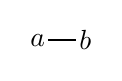
\begin{tikzpicture}[baseline=(a0.base), inner sep=1pt]
      \node (a0) {$a$};
      \node[right=1em of a0] (a1) {$b$};
      \path (a0) edge (a1);
   \end{tikzpicture}
   &
   $y=\sum_i a_i b_i$
   &
   $
\begin{compress}
\left[\begin{array}{cccc}
\cdot & \cdot & \cdot & \cdot \\
\end{array}\right]
\left[\begin{array}{c}
\cdot \\
\cdot \\
\cdot \\
\cdot \\
\end{array}\right]
\end{compress}
   $
   &
   $=y$
   \\
   Outer product
   &
   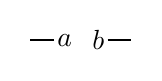
\begin{tikzpicture}[baseline=(a0.base), inner sep=1pt]
      \node (a0) {$a$};
      \node[right=.5em of a0] (a1) {$b$};
      \draw (a0.west) -- ++(-.3,0) node {};
      \draw (a1.east) -- ++(.3,0) node {};
   \end{tikzpicture}
   &
   $Y_{i,j} = a_i b_j$
   &
   $
\begin{compress}
\left[\begin{array}{c}
\cdot \\
\cdot \\
\cdot \\
\cdot \\
\end{array}\right]
\left[\begin{array}{cccc}
\cdot & \cdot & \cdot & \cdot \\
\end{array}\right]
\end{compress}
   $
   &
   $=\mathbin{
   \begin{tikzpicture}[baseline=(Y.base), inner sep=1pt]
      \node (Y) {$Y$};
      \draw (Y.east) -- ++(.3, 0);
      \draw (Y.west) -- ++(-.3, 0);
   \end{tikzpicture}}
   $
   \\
   Matrix-Vector
   &
   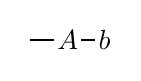
\begin{tikzpicture}[baseline=(A.base), inner sep=1pt]
      \node (A) {$A$};
      \node[right=.5em of A] (b) {$b$};
      \draw (A.west) -- ++(-.3,0) node {};
      \draw (A.east) -- (b.west);
   \end{tikzpicture}
   &
   $
   y_{i} = \sum_j A_{i,j} b_j
   $
   &
   $
   \begin{compress}
   \left[\begin{array}{cccc}
   \cdot & \cdot & \cdot & \cdot \\
   \cdot & \cdot & \cdot & \cdot \\
   \cdot & \cdot & \cdot & \cdot \\
   \cdot & \cdot & \cdot & \cdot \\
   \end{array}\right]
   \left[\begin{array}{c}
   \cdot \\
   \cdot \\
   \cdot \\
   \cdot \\
   \end{array}\right]
   \end{compress}
   $
   &
   $=\mathbin{
   \begin{tikzpicture}[baseline=(y.base), inner sep=1pt]
      \node (y) {$y$};
      \draw (y.west) -- ++(-.3, 0);
   \end{tikzpicture}
   }$
   \\
   Matrix-Matrix
   &
   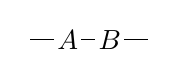
\begin{tikzpicture}[baseline=(A.base), inner sep=1pt]
      \node (A) {$A$};
      \node[right=.5em of A] (B) {$B$};
      \draw (A.west) -- ++(-.3,0) node {};
      \draw (A.east) -- (B.west);
      \draw (B.east) -- ++(.3,0) node {};
   \end{tikzpicture}
   &
   $
   Y_{i,k} = \sum_j A_{i,j} B_{j,k}
   $
   &
   $
   \begin{compress}
   \left[\begin{array}{cccc}
   \cdot & \cdot & \cdot & \cdot \\
   \cdot & \cdot & \cdot & \cdot \\
   \cdot & \cdot & \cdot & \cdot \\
   \cdot & \cdot & \cdot & \cdot \\
   \end{array}\right]
   \left[\begin{array}{cccc}
   \cdot & \cdot & \cdot & \cdot \\
   \cdot & \cdot & \cdot & \cdot \\
   \cdot & \cdot & \cdot & \cdot \\
   \cdot & \cdot & \cdot & \cdot \\
   \end{array}\right]
   \end{compress}
   $
   &
   $=\mathbin{
   \begin{tikzpicture}[baseline=(Y.base), inner sep=1pt]
      \node (Y) {$Y$};
      \draw (Y.west) -- ++(-.3, 0);
      \draw (Y.east) -- ++(.3, 0);
   \end{tikzpicture}
   }$
\end{tabular}
\vspace{.5em}

We think of vectors and matrices as tensors of order 1 and 2.
The order corresponds to the number of dimensions in their $[\cdots]$ visualization above,
e.g. a vector is a 1-dimensional list of numbers, while a matrix is a 2-dimensional grid of numbers.
The order also determines the degree of the node representing the variable in the tensor graph.

Diagram notation becomes more interesting when you have tensors of order 3 and higher.
An order 3 tensor is a cube or numbers, or stack of matrices.
E.g. we can write this as $T\in\R^{n\times m\times k}$, so $T_i\in\R^{m\times k}$ is a matrix for $i=1\dots n$.
Of course we could slice $T$ along the other axes too, so $T_{:,j}\in\R^{n\times k}$ and $T_{:,:,\ell}\in\R^{n\times m}$ are matrices too.

A matrix having two outgoing edges means there are two ways you can multiply a vector onto it, either on the left: $x^T M$, or on the right: $Mx$.
In graph notation we just write $x\!-\!M\!-$ and $-M\!-\!x$.
An order 3 tensor has three edges, so we can multiply it with a vector in three ways:
\[
   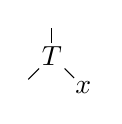
\begin{tikzpicture}[baseline=(T.base), inner sep=1pt]
      \node (T) {$T$};
      \node (x) at (.4,-.4) {$x$};
      \draw (T) -- (x);
      \draw (T) -- ++(-.3,-.3);
      \draw (T) -- ++(0,.35);
   \end{tikzpicture}
   \quad
   \text{and}
   \quad
   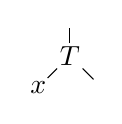
\begin{tikzpicture}[baseline=(T.base), inner sep=1pt]
      \node (T) {$T$};
      \node (x) at (-.4,-.4) {$x$};
      \draw (T) -- (x);
      \draw (T) -- ++(.3,-.3);
      \draw (T) -- ++(0,.35);
   \end{tikzpicture}
   \quad
   \text{and}
   \quad
   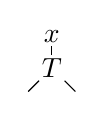
\begin{tikzpicture}[baseline=(T.base), inner sep=1pt]
      \node (T) {$T$};
      \node (x) at (0,.4) {$x$};
      \draw (T) -- (x);
      \draw (T) -- ++(.3,-.3);
      \draw (T) -- ++(-.3,-.3);
   \end{tikzpicture}
\]
To be perfectly precise about what each one means, we should give the edges labels.
For example we would write
$
   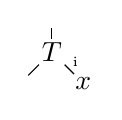
\begin{tikzpicture}[baseline=(T.base), inner sep=1pt]
      \node (T) {$T$};
      \node (x) at (.4,-.4) {$x$};
      \draw (T) -- (x) node[midway, above right, font=\tiny] {i};
      \draw (T) -- ++(-.3,-.3);
      \draw (T) -- ++(0,.3);
   \end{tikzpicture}
$
to specify the matrix $\sum_i T_i x_i$.
However, often the edge in question will be clear from the context, which is part of
what makes tensor diagram notation cleaner than, say, Einstein sum notation.

\[
   Y_{i,j} = \sum_{k,l,m,n,o} A_{i,k} B_{l,n,o} C_{j,k,l,m} D_{m,n} E_o
   \quad
   \Leftrightarrow
   % \quad
   \vcenter{\hbox{
      \import{figures/}{basic_graph.pdf_tex}
   }}
\]

The \emph{key principle} of tensor diagrams is that \emph{edge contraction is associative}.
This means you can contract any edge in any order you prefer.
This can be seen from the sum representation above, which can be reordered to sum over $k,l,m,n$ in any order.

The computational price for different contraction orders can be widely different.
Unfortunately it's not computationally easy to find the optimal order.
See section~\ref{sec:opt_contr} for algorithms to find the best contraction order, and approximate contraction methods.

Note that tensor graphs are not always connected.
We already saw that the outer product of two vectors can be written
   $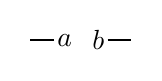
\begin{tikzpicture}[baseline=(a0.base), inner sep=1pt]
      \node (a0) {$a$};
      \node[right=.5em of a0] (a1) {$b$};
      \draw (a0.west) -- ++(-.3,0) node {};
      \draw (a1.east) -- ++(.3,0) node {};
   \end{tikzpicture}$.
This is natural from the sum representation: No edges simply means no sums.
So here $y_{i,j} = a_i b_j$, which is exactly the outer product $y=a\otimes b$.
% Can also mention how this gives us scaling by letter (5) be the order-0 tensor with value 5.


\section{The Copy Tensor}

A particularly important tensor is the ``copy'' tensor, also known as the ``diagonal'', ``kronecker delta'' or ``spider'' tensor.
The simplest version is the all-ones vector, which we write as $\sbullet-$.
That is $\sbullet_i = 1$.
The general order-n tensor is 1 on the diagonal, 0 everywhere else:
\[
   \sbullet_{i,j,k,\ldots} = \begin{cases}
      1\quad \text{if } i=j=k=\dots \\
      0\quad \text {otherwise}
   \end{cases}
\]
% This is also known as the ``copy'' or ``spider'' tensor, or ``generalized Kronecker delta''.
Or, using Iversonian notation, $\sbullet_{i,j,k,\dots} = [i=j=k=\dots]$.
We see the order-2 copy-tensor, $-\sbullet- = I$, is just the identity matrix,
so we can simply remove it from graphs like this:
\[-A\!-\!\sbullet\!-\!B- = -A\!-\!B-\]

Higher order copy-tensors are very useful, because they let us turn the simple tensor graphs into hyper-graphs.
A simple example of how we can use this is the diagonal matrix $D_a$, which has $a$ on the diagonal and 0 elsewhere.
We can write this as
\[
   D_a = 
   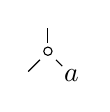
\begin{tikzpicture}[baseline=(T.base), inner sep=1pt]
      \node (T) {$\sbullet$};
      \node (x) at (.3,-.3) {$a$};
      \draw (T) -- (x);
      \draw (T) -- ++(-.25,-.25);
      \draw (T) -- ++(0,.3);
   \end{tikzpicture}
\]
Why?
Because $(D_a)_{i,j} = \sum_k \sbullet_{i,j,k} a_k = \sum_k [i=j=k] a_k = [i=j] a_i$.
Similarly the Hadamard product, $(a\circ b)_i = a_i b_i$, can be written
\[
   a \circ b =
   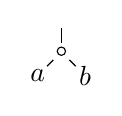
\begin{tikzpicture}[baseline=(T.base), inner sep=1pt]
      \node (T) {$\sbullet$};
      \node (a) at (-.3,-.3) {$a$};
      \node (b) at (.3,-.3) {$b$};
      \draw (T) -- (a);
      \draw (T) -- (b);
      \draw (T) -- ++(0,.3);
   \end{tikzpicture}
\]
Now, let's see why everyone loves copy tensors by using it to
prove the identity $D_aD_b = D_{a\circ b}$ by ``copy tensor manipulation'':
\[
   D_a D_b =
   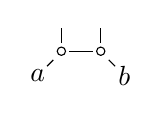
\begin{tikzpicture}[baseline=(T.base), inner sep=1pt]
      \node (T) {$\sbullet$};
      \node (a) at (-.3,-.3) {$a$};
      \draw (T) -- (a);
      \node (T2) at (.5,0) {$\sbullet$};
      \node (b) at (.8,-.3) {$b$};
      \draw (T) -- ++(0,.3);
      \draw (T) -- (T2);
      \draw (T2) -- (b);
      \draw (T2) -- ++(0,.3);
   \end{tikzpicture}
   =
   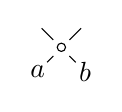
\begin{tikzpicture}[baseline=(T.base), inner sep=1pt]
      \node (T) {$\sbullet$};
      \node (a) at (-.3,-.3) {$a$};
      \node (b) at (.3,-.3) {$b$};
      \draw (T) -- (a);
      \draw (T) -- (b);
      \draw (T) -- ++(.25,.25);
      \draw (T) -- ++(-.25,.25);
   \end{tikzpicture}
   =
   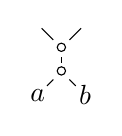
\begin{tikzpicture}[baseline=(T.base), inner sep=1pt]
      \node (T) {$\sbullet$};
      \node (a) at (-.3,-.3) {$a$};
      \node (b) at (.3,-.3) {$b$};
      \draw (T) -- (a);
      \draw (T) -- (b);
      \node (T2) at (0,.3) {$\sbullet$};
      \draw (T) -- (T2);
      \draw (T2) -- ++(.25,.25);
      \draw (T2) -- ++(-.25,.25);
   \end{tikzpicture}
   =
   D_{a\circ b}.
\]
You can verify this using the sum representation.

The general rule at play is that any connected sub-graph of copy-tensors can be combined into a single one.
Sometimes we are even lucky enough that this simplification leaves us with an identity matrix we can remove too:
%\begin{figure}[h]
%   \centering{
   %\def\svgwidth{.5\linewidth}
   %\import{figures/}{path1.pdf_tex}
   %\\
\[
   \def\svgwidth{.75\linewidth}
   \import{figures/}{path2.pdf_tex}
   .
\]
%   \caption{Contracting copy tensors and identity matrices}
%   \label{fig:spiders}
%   }
%\end{figure}
The only time you have to be a bit careful is when the resulting tensor has order 0.
Depending on how you define the order-0 copy tensor, $\sbullet$, you may or may not have the identity $\sbullet\!-\!\sbullet = \sbullet$.

Lots of other constructions that require special notation (like diagonal matrices or Hadamard products) with normal vector notation can be unified using the copy tensor.
%
In the Matrix Cookbook they define the order-4 tensor $J$,
which satisfies $J_{i,j,k,l} = [i=k][j=l]$ and which we'd write as
$J=\vcenter{\hbox{
   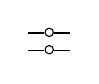
\begin{tikzpicture}[inner sep=0pt]
   \node (a0) {$\sbullet$};
   \draw (a0.east) -- ++(.2,0);
   \draw (a0.west) -- ++(-.2,0);
   \node[below=.2em of a0] (a1) {$\sbullet$};
   \draw (a1.east) -- ++(.2,0);
   \draw (a1.west) -- ++(-.2,0);
\end{tikzpicture}}}$,
and satisfies, for example, $\frac{dX}{dX}=J$.
Using ``tensor products'' you could write $J=I\otimes I$.
Note that $J$ is different from the order-4 copy-tensor,

\begin{tikzpicture}[baseline=(a0.base), inner sep=0pt]
   \node (a0) {$\sbullet$};
   \draw (a0) -- ++(.17,.17);
   \draw (a0) -- ++(.17,-.17);
   \draw (a0) -- ++(-.17,.17);
   \draw (a0) -- ++(-.17,-.17);
\end{tikzpicture}.

\section{Sums of Tensors}

Tensor products can express any linear function.
That is $f$ such that $f(a x, b y) = a b f(x,y)$.
Unfortunately not all operations on tensors are linear.
Even something as simple as a sum of two vectors, $x+y$, can not be displayed with a simple contraction graph.
(Note that this is not linear because $ax+by\neq ab(x+y)$.)

To handle this important operation, Penrose suggesting simply writing the two graphs with a plus sign between them, such as $-x + -y$.
Note that this is itself an order-1 tensor, even though it may look like there are two free edges.
If we want to multiply the sum with another tensor, we can use parentheses like $-M\!-\!(-x + -y)$.

It can be helpful to use named edges when dealing with sums, to make it clear how the edges are matched up.
Sums and tensor products interact nicely, with a general form of the distributive law:
%\begin{figure}[h]
%\centering{
%\def\svgwidth{\linewidth}
\[
\def\svgwidth{.75\linewidth}
\import{figures/}{path3.pdf_tex}
.
\]
%\caption{Distributive law}
%\label{fig:dist}
%}
%\end{figure}

When adding tensors that don't have the same number of edges, or have edges with different names, we can use ``broadcasting''.
%Say we want to add a matrix $\,_i\!-M-_j$ and a vector $x$.
Say we want to add a matrix $M$ and a vector $x$.
What does it even mean?
If we want to add $x$ to every row of $M$, we write
$
\vcenter{\hbox{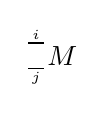
\begin{tikzpicture}[inner sep=1pt]
   \node (M) {$M$};
   \draw (M.north west) -- ++(-.2,0) node[midway, above, font=\tiny] {$i$};
   \draw (M.south west) -- ++(-.2,0) node[midway, below, font=\tiny] {$j$};
\end{tikzpicture}}}
+
\vcenter{\hbox{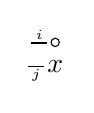
\begin{tikzpicture}[inner sep=1pt]
   \node (a0) {$\sbullet$};
   \draw (a0.west) -- ++(-.2,0) node[midway, above, font=\tiny] {$i$};
   \node[below=.2em of a0] (a1) {$x$};
   \draw (a1.west) -- ++(-.2,0) node[midway, below, font=\tiny] {$j$};
\end{tikzpicture}}}
$.
This is because
$
\vcenter{\hbox{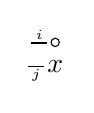
\begin{tikzpicture}[inner sep=1pt]
   \node (a0) {$\sbullet$};
   \draw (a0.west) -- ++(-.2,0) node[midway, above, font=\tiny] {$i$};
   \node[below=.2em of a0] (a1) {$x$};
   \draw (a1.west) -- ++(-.2,0) node[midway, below, font=\tiny] {$j$};
\end{tikzpicture}}}
$
is an outer product between $x$ and the all one vector, which is a matrix in which every row is the same.
Similarly, if we want to add $x$ to every column, we could use
the matrix
$
\vcenter{\hbox{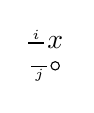
\begin{tikzpicture}[inner sep=1pt]
   \node (a0) {$\sbullet$};
   \draw (a0.west) -- ++(-.2,0) node[midway, below, font=\tiny] {$j$};
   \node[above=.2em of a0] (a1) {$x$};
   \draw (a1.west) -- ++(-.2,0) node[midway, above, font=\tiny] {$i$};
\end{tikzpicture}}}
$.

Note that we typically don't talk about ``rows'' or ``columns'' when dealing with tensors, but simply use the name edge (sometimes axis) of the tensor.
When using named edges, operations from classical vector notation like ``transpose'' can also be removed.
The matrix $X^T$ is simply $X$ where the left and right edge have been swapped.
But if the edges are named, we don't have to keep track on ``where the edge is'' at all.

\section{Trace}

The ``trace'' of a square matrix is defined $\mathrm{Tr}(A) = \sum_i A_{i,i}$.
In tensor diagram notation, that corresponds to a self-edge: $\trace{A}{1}$.
The Matrix Cookbook has a list of identities using traces.
Let's reproduce them with tensor diagrams:
\begin{align*}
   \sum_{i=1}^{n} A_{ii} &= \mathrm{Tr}(A) = \mathrm{Tr}(A I)
   &
   \trace{A}{1} &= \trace{A, \sbullet}{2}
   \tag{11}
   \\%%%%%%%%%%%%%%%%%%%%%%%%%%%%%%%%%%%%%%%%
   \mathrm{Tr}(A) &= \sum_i \lambda_i = \langle 1, \lambda\rangle
   &
   \trace{A}1 &=
   \hspace{-2em}
   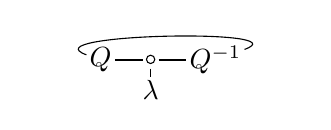
\begin{tikzpicture}[baseline=(Q.base), inner sep=1pt]
      \node (Q) {$Q$};
      \node[right=1em of Q] (dot) {$\sbullet$};
      \path (Q) edge (dot);
      \node[below=.3em of dot] (e) {$\lambda$};
      \path (dot) edge (e);
      \node[right=1em of dot] (Qi) {$Q^{-1}$};
      \path (dot) edge (Qi);
      \path (Q) edge [out=160, in=20, looseness=1] (Qi);
   \end{tikzpicture}
   \hspace{-2em}
   \tag{12}
   \\%%%%%%%%%%%%%%%%%%%%%%%%%%%%%%%%%%%%%%%%
   \mathrm{Tr}(A) &= \mathrm{Tr}(A^T)
   &
   \trace{A}1 &= \trace{A}1
   \tag{13}
   \\%%%%%%%%%%%%%%%%%%%%%%%%%%%%%%%%%%%%%%%%
   \mathrm{Tr}(AB) &= \mathrm{Tr}(BA)
   &
   \trace{A,B}2 &= \trace{B,A}2
   \tag{14}
   \\%%%%%%%%%%%%%%%%%%%%%%%%%%%%%%%%%%%%%%%%
   \tag{15}
   \mathrm{Tr}(A+B)
   &= \mathrm{Tr}(A) + \mathrm{Tr}(B)
   &
   \trace{(A+B),\sbullet}1
   %\trace{(\matmul{A}+\matmul{B}),\sbullet}{2}
   &= \trace{A,\sbullet}2
 \\&&&+\trace{B,\sbullet}2
   \\%%%%%%%%%%%%%%%%%%%%%%%%%%%%%%%%%%%%%%%%
   \tag{16}
   \mathrm{Tr}(ABC) &= \mathrm{Tr}(BCA)
   &
   \trace{A,B,C}1 &= \trace{B,C,A}1
   \\
                  & = \mathrm{Tr}(CAB)
                  &&= \trace{C,A,B}1
   \\[0.5em]
   %%%%%%%%%%%%%%%%%%%%%%%%%%%%%%%%%%%%%%%%
   \tag{17}
   a^T a &= \mathrm{Tr}(a a^T)
   &
   \vecmatvec{1em}{a}{}{a}
   &=
   \mathrm{Tr}(
   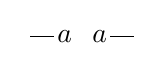
\begin{tikzpicture}[baseline=(a0.base), inner sep=1pt]
      \node (a0) {$a$};
      \node[right=.5em of a0] (a1) {$a$};
      \draw (a0.west) -- ++(-.3,0) node {};
      \draw (a1.east) -- ++(.3,0) node {};
   \end{tikzpicture}
   )
 \\&&&=
   \hspace{-1em}
   
\begin{tikzpicture}[baseline=(a0.base), inner sep=1pt]
      \node (a0) {$a$};
      \node[right=1em of a0] (a1) {$a$};
      \path (a0) edge [out=160, in=20, looseness=2] (a1);
   \end{tikzpicture}
   \hspace{-1em}
\end{align*}



\section{Eigenvalues}
TODO: What else does the Matrix Cookbook include here?
\begin{tikzpicture}[baseline=(A.base), inner sep=1pt]
   \node (A) {$A$};
   \draw (A.west) -- ++(-.3, 0);
   \draw (A.east) -- ++(+.3, 0);
\end{tikzpicture}
=
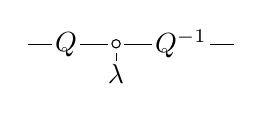
\begin{tikzpicture}[baseline=(Q.base), inner sep=1pt]
   \node (Q) {$Q$};
   \draw (Q.west) -- ++(-.3, 0);
   \node[right=1em of Q] (dot) {$\sbullet$};
   \path (Q) edge (dot);
   \node[below=.3em of dot] (e) {$\lambda$};
   \path (dot) edge (e);
   \node[right=1em of dot] (Qi) {$Q^{-1}$};
   \path (dot) edge (Qi);
   \draw (Qi.east) -- ++(.3, 0);
\end{tikzpicture}
where $\lambda_i$ is the $i$th eigenvalue of $A$.


%\begin{enumerate}
   %\item Contractions are associative: You can contract edges in any order.
   %\item distributive law of sums/products.
   %\item Sums and broadcasting.
   %\item You can always contract connected subgraphs of Copy tensors.
%\end{enumerate}

\section{Exercises}
\begin{exercise}
   Given a sequence of matrices $A_1, A_2, \ldots, A_n \in \mathbb R^{n\times n}$,
   and vectors $v_1, v_2, \ldots, v_n \in \mathbb R^n$,
   draw, using tensor diagrams, the matrix made of vectors $A_1v_1, A_2v_2, \ldots, A_nv_n$.
\end{exercise}

% 
\chapter{Simple Derivatives}

A derivative with respect to a tensor is simply the collection of derivatives with respect to each element of this tensor.
We can keep track of $\frac{d T}{d U}$ by making a tensor of shape $\mathrm{shape}(T) \cup \mathrm{shape}(U)$.
For example, if $T$ is an order-3 tensor and $U$ is an order-2 tensor, we draw $dT/dU$ as
\[
   \frac{dT}{dU} =
   \vcenter{\hbox{
      \import{figures/}{dTdU.pdf_tex}
   }}
\]
This notation follows Penrose.
The two extra lines coming from the black dot on the circle makes the derivative an order-5 tensor.
That the order of derivatives grows this way, is one of the main reasons we'll encounter for tensors to show up in the first place.

When there are not too many edges, we will use a simple inline notation like this:
\[
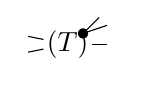
\begin{tikzpicture}[baseline=(T.base), inner sep=1pt]
   \node (T) {$(T)$};
   \draw (T) -- ++(-.5,-.1);
   \draw (T) -- ++(-.5,+.1);
   \draw (T) -- ++(+.5,0);
   \draw[d] (T.east) -- ++(.2,.2);
   \draw[d] (T.east) -- ++(.3,.1);
\end{tikzpicture}
\]

The Matrix Cookbook defines the single-entry matrix $J^{i,j} \in R^{n\times n}$ as the matrix which is zero everywhere except in the entry $(i, j)$ in which it is 1.
Alternatively we could write $J^{i,j}_{n,m} = [i=n][j=m]$.

\section{Derivatives of Matrices, Vectors and Scalar Forms}

\subsection{First Order}
The following first order derivatives show the basic linearity properties of the derivative operator.

\begin{align*}
   \tag{69}
   \frac{\partial x^T a}{\partial x}
   &= \frac{\partial a^T x}{\partial x}
   = a
   &
      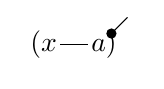
\begin{tikzpicture}[baseline=(a0.base), inner sep=1pt]
         \node (a0) {$(x$};
         \node[right=1em of a0] (a1) {$a)$};
         \path (a0) edge (a1);
         \draw [d] (a1.east) -- ++(.2,.2);
      \end{tikzpicture}
   &=
      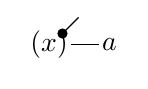
\begin{tikzpicture}[baseline=(a0.base), inner sep=1pt]
         \node (a0) {$(x)$};
         \node[right=1em of a0] (a1) {$a$};
         \path (a0) edge (a1);
         \draw [d] (a0.east) -- ++(.2,.2);
      \end{tikzpicture}
   =
      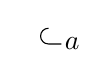
\begin{tikzpicture}[baseline=(a0.base), inner sep=1pt]
         \node (a0) {};
         \node[right=1em of a0] (a1) {$a$};
         \draw (a1) -- ++(-.3, 0) arc (-90:-270:.1);
      \end{tikzpicture}
   =
      \begin{tikzpicture}[baseline=(a.base), inner sep=1pt]
         \draw (0,0) node[left] {$a$} -- ++(.3, 0);
      \end{tikzpicture}
   \\
   %%%%%%%%%%%%%%%%%%%%%%%%%%%%%%%%%%%%%%%%
   \tag{70}
   \frac{\partial a^T X b}{\partial X} &= ab^T
   &
      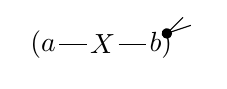
\begin{tikzpicture}[baseline=(a0.base), inner sep=1pt]
         \node (a0) {$(a$};
         \node[right=1em of a0] (a1) {$X$};
         \node[right=1em of a1] (a2) {$b)$};
         \path (a0) edge (a1);
         \path (a1) edge (a2);
         \draw[d] (a2.east) -- ++(.2,.2);
         \draw[d] (a2.east) -- ++(.3,.1);
      \end{tikzpicture}
   &=
      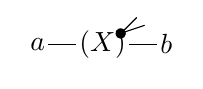
\begin{tikzpicture}[baseline=(a0.base), inner sep=1pt]
         \node (a0) {$a$};
         \node[right=1em of a0] (a1) {$(X)$};
         \node[right=1em of a1] (a2) {$b$};
         \path (a0) edge (a1);
         \path (a1) edge (a2);
         \draw[d] (a1.east) -- ++(.2,.2);
         \draw[d] (a1.east) -- ++(.3,.1);
      \end{tikzpicture}
      =
      \begin{tikzpicture}[baseline=(a0.base), inner sep=1pt]
         \node (a) {$a$};
         \draw (a) -- ++(.3, 0) arc (270:90:-.1);
         \node[right=2em of a] (b) {$b$};
         \draw (b) -- ++(-.3, 0) arc (270:90:.1);
      \end{tikzpicture}
   \\
   %%%%%%%%%%%%%%%%%%%%%%%%%%%%%%%%%%%%%%%%
   \tag{73}
   \frac{\partial X}{\partial X_{i,j}} &= J^{i,j}
   &
      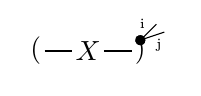
\begin{tikzpicture}[baseline=(a0.base), inner sep=1pt]
         \node (a0) {$($};
         \node[right=1em of a0] (a1) {$X$};
         \node[right=1em of a1] (a2) {$)$};
         \path (a0) edge (a1);
         \path (a1) edge (a2);
         \draw[d] (a2.east) -- ++(.2,.2) node[midway, above left, font=\tiny] {i};
         \draw[d] (a2.east) -- ++(.3,.1) node[midway, below right, font=\tiny] {j};
      \end{tikzpicture}
   &=
      \begin{tikzpicture}[baseline=(a0.base), inner sep=1pt]
         \node (a0) {};
         \node[right=1em of a0] (a1) {};
         \node[right=1em of a1] (a2) {};
         \path (a0) edge (a1);
         \path (a1) edge (a2);
         \draw (a1.west) -- ++(.1,.2) node[midway, above left, font=\tiny] {i};
         \draw (a1.east) -- ++(-.1,-.2) node[midway, below right, font=\tiny] {j};
      \end{tikzpicture}
   \\
   %%%%%%%%%%%%%%%%%%%%%%%%%%%%%%%%%%%%%%%%
   \tag{74}
   \frac{\partial (X A)_{i,j}}{\partial X_{m,n}} &= (J^{m,n} A)_{i,j}
   &
      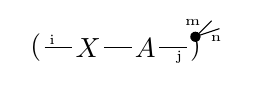
\begin{tikzpicture}[baseline=(a0.base), inner sep=1pt]
         \node (a0) {$($};
         \node[right=1em of a0] (a1) {$X$};
         \node[right=1em of a1] (a2) {$A$};
         \node[right=1em of a2] (a3) {$)$};
         \draw (a0) -- (a1) node[midway, above left, font=\tiny] {i};
         \draw (a1) -- (a2);
         \draw (a2) -- (a3) node[midway, below right, font=\tiny] {j};
         \draw[d] (a3.east) -- ++(.2,.2) node[midway, above left, font=\tiny] {m};
         \draw[d] (a3.east) -- ++(.3,.1) node[midway, below right, font=\tiny] {n};
      \end{tikzpicture}
   &=
      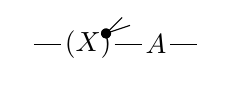
\begin{tikzpicture}[baseline=(a0.base), inner sep=1pt]
         \node (a0) {};
         \node[right=1em of a0] (a1) {$(X)$};
         \node[right=1em of a1] (a2) {$A$};
         \node[right=1em of a2] (a3) {};
         \path (a0) edge (a1);
         \path (a1) edge (a2);
         \path (a2) edge (a3);
         \draw[d] (a1.east) -- ++(.2,.2);
         \draw[d] (a1.east) -- ++(.3,.1);
      \end{tikzpicture}
 \\&&&=
      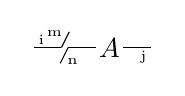
\begin{tikzpicture}[baseline=(a0.base), inner sep=1pt]
         \node (a0) {};
         \node[right=1em of a0] (a1) {};
         \node[right=1em of a1] (a2) {$A$};
         \node[right=1em of a2] (a3) {};
         \draw (a0) -- (a1) node[midway, above left, font=\tiny] {i};
         \draw (a1) -- (a2);
         \draw (a2) -- (a3) node[midway, below right, font=\tiny] {j};
         \draw (a1.west) -- ++(.1,.2) node[midway, above left, font=\tiny] {m};
         \draw (a1.east) -- ++(-.1,-.2) node[midway, below right, font=\tiny] {n};
      \end{tikzpicture}
\end{align*}

\subsection{Second Order}
The second order derivatives are follow from the product rule:
\[
   \vcenter{\hbox{
      \import{figures/}{product.pdf_tex}
   }}
\]
Note that this rule holds independently of how many edges are between $T$ and $U$, even if there are none.

\noindent
%\makebox[\textwidth]{\parbox{1.1\textwidth}{%
\begin{adjustwidth}{-0.05\textwidth}{-0.05\textwidth}
\begin{align*}
   \tag{76}
   \frac{\partial}{\partial X_{i,j}}
   \sum_{k,l,m,n} X_{k,l} X_{m,n}
   &= (\sum_{k,l} X_{k,l})^2
   %&= \frac{\partial \|X\|_F^2}{\partial X_{i,j}}
   %&= 2\, \sum_{k,l} X_{k,l}
   &
   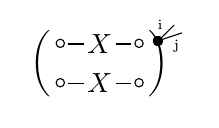
\begin{tikzpicture}[baseline=.5em, inner sep=1pt]
      \node (a0) at (0,0) {$\sbullet$};
      \node (a1) at (.5,0) {$X$};
      \node (a2) at (1,0) {$\sbullet$};
      \path (a0) edge (a1);
      \path (a1) edge (a2);
      \node (b0) at (0, .5) {$\sbullet$};
      \node (b1) at (.5, .5) {$X$};
      \node (b2) at (1, .5) {$\sbullet$};
      \path (b0) edge (b1);
      \path (b1) edge (b2);
      \node at (-.25, .25) {$\bigg($};
      \node at (1.25, .25) {$\bigg)$};
      \draw[d] (1.35, .4) -- ++(.2,.2) node[midway, above left, font=\tiny] {i};
      \draw[d] (1.35, .4) -- ++(.3,.1) node[midway, below right, font=\tiny] {j};
   \end{tikzpicture}
   &=
   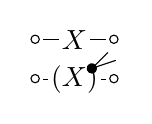
\begin{tikzpicture}[baseline=.5em, inner sep=1pt]
      \node (a0) at (0,0) {$\sbullet$};
      \node (a1) at (.5,0) {$(X)$};
      \node (a2) at (1,0) {$\sbullet$};
      \path (a0) edge (a1);
      \path (a1) edge (a2);
      \node (b0) at (0, .5) {$\sbullet$};
      \node (b1) at (.5, .5) {$X$};
      \node (b2) at (1, .5) {$\sbullet$};
      \path (b0) edge (b1);
      \path (b1) edge (b2);
      \draw[d] (.83,.0) -- ++(.2,.2);
      \draw[d] (.83,.0) -- ++(.3,.1);
   \end{tikzpicture}
   +
   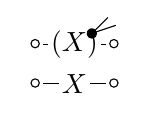
\begin{tikzpicture}[baseline=.5em, inner sep=1pt]
      \node (a0) at (0,0) {$\sbullet$};
      \node (a1) at (.5,0) {$X$};
      \node (a2) at (1,0) {$\sbullet$};
      \path (a0) edge (a1);
      \path (a1) edge (a2);
      \node (b0) at (0, .5) {$\sbullet$};
      \node (b1) at (.5, .5) {$(X)$};
      \node (b2) at (1, .5) {$\sbullet$};
      \path (b0) edge (b1);
      \path (b1) edge (b2);
      \draw[d] (0.83,.5) -- ++(.2,.2);
      \draw[d] (0.83,.5) -- ++(.3,.1);
   \end{tikzpicture}
   %\\[.3em]
   \\
   &= 2\, \sum_{k,l} X_{k,l}
   &&=
   2\,
   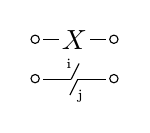
\begin{tikzpicture}[baseline=.5em, inner sep=1pt]
      \node (a0) at (0,0) {$\sbullet$};
      \node (a1) at (.5,0) {};
      \node (a2) at (1,0) {$\sbullet$};
      \path (a0) edge (a1);
      \path (a1) edge (a2);
      \node (b0) at (0, .5) {$\sbullet$};
      \node (b1) at (.5, .5) {$X$};
      \node (b2) at (1, .5) {$\sbullet$};
      \path (b0) edge (b1);
      \path (b1) edge (b2);
      \draw (a1.west) -- ++(.1,.2) node[midway, above left, font=\tiny] {i};
      \draw (a1.east) -- ++(-.1,-.2) node[midway, below right, font=\tiny] {j};
   \end{tikzpicture}
   %%%%%%%%%%%%%%%%%%%%%%%%%%%%%%%%%%%%%%%%
   \\[.5em]
   \tag{77} 
   \frac{\partial b^T X^T X c}{\partial X} &= X(bc^T + cb^T) 
   &
   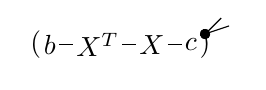
\begin{tikzpicture}[baseline=(a0.base), inner sep=1pt]
      \node (a0) {$(\vecmatvec{.5em}{b}{X^T,X}{c})$};
      \draw[d] (a0.east) -- ++(.2,.2);
      \draw[d] (a0.east) -- ++(.3,.1);
   \end{tikzpicture}
   &=
   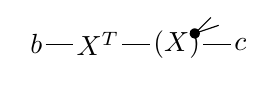
\begin{tikzpicture}[baseline=(a0.base), inner sep=1pt]
      \node (a0) {$b$};
      \node[right=1em of a0] (a1) {$X^T$};
      \node[right=1em of a1] (a2) {$(X)$};
      \node[right=1em of a2] (a3) {$c$};
      \draw (a0) -- (a1);
      \draw (a1) -- (a2);
      \draw (a2) -- (a3);
      \draw[d] (a2.east) -- ++(.2,.2);
      \draw[d] (a2.east) -- ++(.3,.1);
   \end{tikzpicture}
 \\&&&+
   \begin{tikzpicture}[baseline=(a0.base), inner sep=1pt]
      \node (a0) {$b$};
      \node[right=1em of a0] (a1) {$(X^T)$};
      \node[right=1em of a1] (a2) {$X$};
      \node[right=1em of a2] (a3) {$c$};
      \draw (a0) -- (a1);
      \draw (a1) -- (a2);
      \draw (a2) -- (a3);
      \draw[d] (a1.east) -- ++(.2,.2);
      \draw[d] (a1.east) -- ++(.3,.1);
   \end{tikzpicture}
   \\[.3em]&&&=
   \begin{tikzpicture}[baseline=(a0.base), inner sep=1pt]
      \node (a0) {$b$};
      \node[right=1em of a0] (a1) {$X^T$};
      \node[right=1em of a1] (a2) {};
      \node[right=1em of a2] (a3) {$c$};
      \draw (a0) -- (a1);
      \draw (a1) -- (a2);
      \draw (a2) -- (a3);
      \draw (a2.west) -- ++(.1,.2);
      \draw (a2.east) -- ++(-.1,-.2);
   \end{tikzpicture}
 \\&&&+
   \begin{tikzpicture}[baseline=(a0.base), inner sep=1pt]
      \node (a0) {$b$};
      \node[right=1em of a0] (a1) {};
      \node[right=1em of a1] (a2) {$X$};
      \node[right=1em of a2] (a3) {$c$};
      \draw (a0) -- (a1);
      \draw (a1) -- (a2);
      \draw (a2) -- (a3);
      \draw (a1.west) -- ++(.1,.2);
      \draw (a1.east) -- ++(-.1,-.2);
   \end{tikzpicture}
   \\[.3em]&&&=
   \begin{tikzpicture}[baseline=(a0.base), inner sep=1pt]
      \node (a0) {$X$};
      \node[right=.7em of a0] (a1) {$($};
      \node[right=.4em of a1] (a2) {$b\, c$};
      \node[right=.4em of a2] (a4) {$+$};
      \node[right=.6em of a4] (a5) {$c\, b$};
      \node[right=.2em of a5] (a7) {$)$};
      \draw (a0.west) -- ++(-.2,0);
      \draw (a0) -- (a1);
      \draw (a2.west) -- ++(-.2,0);
      \draw (a2.east) -- ++(.1,.15);
      \draw (a5.west) -- ++(-.2,0);
      \draw (a5.east) -- ++(.1,.15);
   \end{tikzpicture}
   \\
   \tag{79} 
   \frac{\partial}{\partial X_{i,j}} (X^TBX)_{k,l} &= \delta_{l,j}(X^TB)_{k,i}
   %  \\&+ \delta_{k,j}(BX)_{i,l} 
   &
   \begin{tikzpicture}[baseline=(a0.base), inner sep=1pt]
      \node (a0) {$($};
      \node[right=.5em of a0] (a1) {$X^T$};
      \node[right=.5em of a1] (a2) {$B$};
      \node[right=.5em of a2] (a3) {$X$};
      \node[right=.5em of a3] (a4) {$)$};
      \draw (a0) -- (a1) node[midway, above left, font=\tiny] {k};
      \draw (a1) -- (a2);
      \draw (a2) -- (a3);
      \draw (a3) -- (a4) node[midway, below right, font=\tiny] {l};
      \draw[d] (a4.east) -- ++(.2,.2) node[midway, above left, font=\tiny] {i};
      \draw[d] (a4.east) -- ++(.3,.1) node[midway, below right, font=\tiny] {j};
   \end{tikzpicture}
   &=
   \begin{tikzpicture}[baseline=(a0.base), inner sep=1pt]
      \node (a0) {};
      \node[right=.5em of a0] (a1) {$X^T$};
      \node[right=.5em of a1] (a2) {$B$};
      \node[right=.5em of a2] (a3) {};
      \node[right=.5em of a3] (a4) {};
      \draw (a0) -- (a1) node[midway, above left, font=\tiny] {k};
      \draw (a1) -- (a2);
      \draw (a2) -- (a3);
      \draw (a3) -- (a4) node[midway, below right, font=\tiny] {l};
      \draw (a3.west) -- ++(.1,.2) node[midway, above left, font=\tiny] {i};
      \draw (a3.east) -- ++(-.1,-.2) node[midway, below right, font=\tiny] {j};
   \end{tikzpicture}
   \\
   &+ \delta_{k,j}(BX)_{i,l}
   &&+
   \begin{tikzpicture}[baseline=(a0.base), inner sep=1pt]
      \node (a0) {};
      \node[right=.5em of a0] (a1) {};
      \node[right=.5em of a1] (a2) {$B$};
      \node[right=.5em of a2] (a3) {$X$};
      \node[right=.5em of a3] (a4) {};
      \draw (a0) -- (a1) node[midway, above left, font=\tiny] {k};
      \draw (a1) -- (a2);
      \draw (a2) -- (a3);
      \draw (a3) -- (a4) node[midway, below right, font=\tiny] {l};
      \draw (a1.west) -- ++(.1,.2) node[midway, above left, font=\tiny] {j};
      \draw (a1.east) -- ++(-.1,-.2) node[midway, below right, font=\tiny] {i};
   \end{tikzpicture}
   %%%%%%%%%%%%%%%%%%%%%%%%%%%%%%%%%%%%%%%%
   \\
   \tag{80} 
   \frac{\partial}{\partial X_{i,j}} X^TBX &= X^TBJ^{i,j} + J^{j,i}BX 
   &
   \text{(same as above)} &
   %%%%%%%%%%%%%%%%%%%%%%%%%%%%%%%%%%%%%%%%
   \\
   \tag{81} 
   \frac{\partial}{\partial x} x^TBx &= (B+B^T)x 
   &
   \begin{tikzpicture}[baseline=(a0.base), inner sep=1pt]
      \node (a0) {$(x$};
      \node[right=.5em of a0] (a1) {$B$};
      \node[right=.5em of a1] (a2) {$x)$};
      \draw (a0) -- (a1);
      \draw (a1) -- (a2);
      \draw[d] (a2.east) -- ++(.2,.2) node[midway, above left, font=\tiny] {i};
      \draw[d] (a2.east) -- ++(.3,.1) node[midway, below right, font=\tiny] {j};
   \end{tikzpicture}
   &=
   \vecmatvec{.5em}{}{B}{x}
   + \vecmatvec{.5em}{x}{B}{}
 \\&&&=
   \begin{tikzpicture}[baseline=.5em, inner sep=1pt]
      \node (a0) at (0,0) {};
      \node (a1) at (.5,0) {$B$};
      \node (a2) at (1,0) {};
      \draw (a0) -- (a1) node[midway, below left, font=\tiny] {i};
      \draw (a1) -- (a2) node[midway, below right, font=\tiny] {j};
      \node (b0) at (0, .5) {};
      \node (b1) at (.5, .5) {$B$};
      \node (b2) at (1, .5) {};
      \draw (b0) -- (b1) node[midway, above left, font=\tiny] {j};
      \draw (b1) -- (b2) node[midway, above right, font=\tiny] {i};
      \node (l) at (-.3, .25) {$\bigg($};
      \node at (1.15, .25) {$\bigg)$};
      \node at (-.1, .25) {$+$};
      \node (x) at (-1,.25) {$x$};
      \draw (x) -- (l) node[midway, above right, font=\tiny] {i};
   \end{tikzpicture}
\end{align*}
\end{adjustwidth}
%}}


TODO: Assume $W$ is symmetric, then... (84) - (88)

\subsection{Higher Order}
Integer powers of matrices, like $X^n$, are easy to handle by writing
out the product and using the product rule.
The Matrix Cookbook includes a few derivatives we can handle this way.
\begin{align*}
   \\[.5em]
   %\tag{77} 
   %\frac{\partial b^T X^T X c}{\partial X} &= X(bc^T + cb^T) 
   \frac{\partial\left(\mathbf{X}^n\right)_{k l}}{\partial X_{i j}}
   &=
  \sum_{r=0}^{n-1}\left(\mathbf{X}^r \mathbf{J}^{i j} \mathbf{X}^{n-1-r}\right)_{k l}
   &&
   \begin{tikzpicture}[baseline=(X0.base), inner sep=1pt]
      \node (X0) {$(X$};
      \node[right=.25 of X0] (X1) {$X$};
      \node[right=.25 of X1] (X2) {$X$};
      \node[right=.25 of X2] (X3) {$\dots$};
      \node[right=.25 of X3] (X4) {$X)$};
      \draw (X0) -- ++(-.5,0) node[midway, above left, font=\tiny] {k};
      \draw (X0) -- (X1) -- (X2) -- (X3) -- (X4);
      \draw (X4) -- ++(.5,0) node[midway, below right, font=\tiny] {l};
      \draw[d] (X4.east) -- ++(.2,.2)node[midway, above left, font=\tiny]{i};
      \draw[d] (X4.east) -- ++(.3,.1)node[midway, below right, font=\tiny]{j};
   \end{tikzpicture}
   \\
   &&&=\quad
   \begin{tikzpicture}[baseline=(X0.base), inner sep=1pt]
      \node (X0) {$(X)$};
      \node[right=.25 of X0] (X1) {$X$};
      \node[right=.25 of X1] (X2) {$X$};
      \node[right=.25 of X2] (X3) {$\dots$};
      \node[right=.25 of X3] (X4) {$X$};
      \draw (X0) -- ++(-.5,0) node[midway, above left, font=\tiny] {k};
      \draw (X0) -- (X1) -- (X2) -- (X3) -- (X4);
      \draw (X4) -- ++(.5,0) node[midway, below right, font=\tiny] {l};
      \draw[d] (X0.east) -- ++(.2,.2)node[midway, above left, font=\tiny]{i};
      \draw[d] (X0.east) -- ++(.3,.1)node[midway, below right, font=\tiny]{j};
   \end{tikzpicture}
 \\&&&+\quad\dots
 \\&&&+\quad
   \begin{tikzpicture}[baseline=(X0.base), inner sep=1pt]
      \node (X0) {$X$};
      \node[right=.25 of X0] (X1) {$X$};
      \node[right=.25 of X1] (X2) {$X$};
      \node[right=.25 of X2] (X3) {$\dots$};
      \node[right=.25 of X3] (X4) {$(X)$};
      \draw (X0) -- ++(-.5,0) node[midway, above left, font=\tiny] {k};
      \draw ++(-.5,0) -- (X0) -- (X1) -- (X2) -- (X3) -- (X4);
      \draw (X4) -- ++(.5,0) node[midway, below right, font=\tiny] {l};
      \draw[d] (X4.east) -- ++(.2,.2)node[midway, above left, font=\tiny]{i};
      \draw[d] (X4.east) -- ++(.3,.1)node[midway, below right, font=\tiny]{j};
   \end{tikzpicture}
 \\&&&=\quad
 \sum_{r=0}^{n-1}
   \begin{tikzpicture}[baseline=(X0.base), inner sep=1pt]
      \node (X0) {$X^r$};
      \node[right=.5 of X0] (X1) {$X^{n-r-1}$};
      \draw (X0.west) -- ++(-.25,0) node[midway, above left, font=\tiny] {k};
      \draw (X0.east) -- ++(.2,0) -- ++(.1,.2) node[midway, above left, font=\tiny] {i};
      \draw (X1.east) -- ++(.25,0) node[midway, below right, font=\tiny] {l};
      \draw (X1.west) -- ++(-.2,0) -- ++(-.1,-.2) node[midway, below right, font=\tiny] {j};
   \end{tikzpicture}
 \\
   \frac{\partial}{\partial \mathbf{X}} \mathbf{a}^T \mathbf{X}^n \mathbf{b}
   &=\sum_{r=0}^{n-1}\left(\mathbf{X}^r\right)^T \mathbf{a b}^T\left(\mathbf{X}^{n-1-r}\right)^T
   &&
   \begin{tikzpicture}[baseline=(X0.base), inner sep=1pt]
      \node (X0) {$(a-X$};
      \node[right=.25 of X0] (X3) {$\dots$};
      \node[right=.25 of X3] (X4) {$X-b)$};
      \draw (X0) -- (X3) -- (X4);
      \draw[d] (X4.east) -- ++(.2,.2);
      \draw[d] (X4.east) -- ++(.3,.1);
   \end{tikzpicture}
   \\
   &&&=\quad
   \sum_{r=0}^{n-1}
   \begin{tikzpicture}[baseline=(X0.base), inner sep=1pt]
      \node (X0) {$a-X^r$};
      \node[right=.5 of X0] (X1) {$X^{n-r-1}-b$};
      \draw (X0.east) -- ++(.25,.05) -- ++(-.1,.1);
      \draw (X1.west) -- ++(-.25,-.05) -- ++(.1,-.1);
   \end{tikzpicture}
   \\
   &&&=\quad
   \sum_{r=0}^{n-1}
   \begin{tikzpicture}[baseline=(X0.base), inner sep=1pt]
      \node (X0) {$-(X^r)^T-a$};
      \node[right=.25 of X0] (X1) {$b-(X^{n-r-1})^T-$};
   \end{tikzpicture}
\end{align*}


% Could be cool to do exponential here, if I could only find a good result for it...
% sum_{t>=1} 1/t! sum_{a+b=t-1} X^a X^b
% sum_{t>=1, a+b=t-1} X^a X^b / t!
% sum_{a>=0} sum_{b>=0} X^a X^b / (a+b+1)!


\section{Derivatives of Traces}
The Matrix Cookbook contains a lot of derivatives for traces.
These can be elegant in classical notation, since traces are scalar, so the derivatives are low order.

\subsection{First Order}

\begin{align*}
   \tag{99}
   \frac{\partial}{\partial X} \mathrm{Tr}(X)
   &= I
   &
   \hspace{-1em}
   \begin{tikzpicture}[baseline=(a0.base), inner sep=1pt]
      \node (a0) {$($};
      \node[right=1em of a0] (a1) {$X$};
      \node[right=1em of a1] (a3) {$)$};
      \path (a1) edge[out=160, in=20, loop] (a1);
      \draw[d] (a3.east) -- ++(.2,.2);
      \draw[d] (a3.east) -- ++(.3,.1);
   \end{tikzpicture}
   \hspace{-1em}
   &=
   \hspace{-2em}
   \begin{tikzpicture}[baseline=(a0.base), inner sep=1pt]
      \node (a1) {$(X)$};
      \path (a1) edge[out=160, in=20, loop, looseness=4] (a1);
      \draw[d] (a1.south east) -- ++(.2,-.2);
      \draw[d] (a1.south east) -- ++(.3,-.1);
   \end{tikzpicture}
   \hspace{-2em}
 \\&&&=
   \hspace{-1.5em}
   \begin{tikzpicture}[baseline=(a0.base), inner sep=1pt]
      \node (a1) {$\phantom{X}$};
      \path (a1) edge[out=160, in=20, loop, looseness=6] (a1);
      \draw ($(a1.east)-(0,-.2em)$) -- ++(.2,-.1);
      \draw ($(a1.west)-(0,-.2em)$) -- ++(-.2,-.1);
   \end{tikzpicture}
   \hspace{-1.5em}
 \\&&&=
   \matmul{\sbullet}
   %%%%%%%%%%%%%%%%%%%%%%%%%%%%%%
   \\
   \tag{100}
   \frac{\partial}{\partial X} \mathrm{Tr}(XA)
   &= A^T
   &
   \begin{tikzpicture}[baseline=(a0.base), inner sep=1pt]
      \node (a0) {$($};
      \node[right=1em of a0] (a1) {$X$};
      \node[right=1em of a1] (a2) {$A$};
      \node[right=1em of a2] (a3) {$)$};
      \draw (a1) -- (a2);
      \path (a1) edge[out=160, in=20, looseness=2] (a2);
      \draw[d] (a3.east) -- ++(.2,.2);
      \draw[d] (a3.east) -- ++(.3,.1);
   \end{tikzpicture}
   &=
   \hspace{-2em}
   \begin{tikzpicture}[baseline=(a0.base), inner sep=1pt]
      \node (a1) {$(X)$};
      \node[right=1em of a1] (a2) {$A$};
      \draw (a1) -- (a2);
      \path (a1) edge[out=160, in=20, looseness=2] (a2);
      \draw[d] (a1.south east) -- ++(.2,-.2);
      \draw[d] (a1.south east) -- ++(.3,-.1);
   \end{tikzpicture}
   \hspace{-2em}
 \\&&&=
   \hspace{-1.5em}
   \begin{tikzpicture}[baseline=(a0.base), inner sep=1pt]
      \node (a1) {$\phantom{X}$};
      \node[right=1em of a1] (a2) {$A$};
      \draw (a1) -- (a2);
      \path (a1) edge[out=160, in=20, looseness=2] (a2);
      \draw (a1.east) -- ++(.2,-.1);
      \draw ($(a1.west)-(0,-.2em)$) -- ++(-.2,-.1);
   \end{tikzpicture}
   \hspace{-1.5em}
 \\&&&
   = \matmul{A^T}
   %%%%%%%%%%%%%%%%%%%%%%%%%%%%%%
   \\
   \tag{101}
   \frac{\partial}{\partial X} \mathrm{Tr}(AXB)
   &= A^TB^T
   &
   \hspace{-1em}
   \begin{tikzpicture}[baseline=(a0.base), inner sep=1pt]
      \node (a0) {$($};
      \node[right=1em of a0] (a1) {$A$};
      \node[right=1em of a1] (a2) {$X$};
      \node[right=1em of a2] (a3) {$B$};
      \node[right=1em of a3] (a4) {$)$};
      \draw (a1) -- (a2) -- (a3);
      \path (a1) edge[out=160, in=20, looseness=1] (a3);
      \draw[d] (a4.east) -- ++(.2,.2);
      \draw[d] (a4.east) -- ++(.3,.1);
   \end{tikzpicture}
   &=
   \hspace{-1em}
   \begin{tikzpicture}[baseline=(a0.base), inner sep=1pt]
      \node (a1) {$A$};
      \node[right=1em of a1] (a2) {$(X)$};
      \node[right=1em of a2] (a3) {$B$};
      \draw (a1) -- (a2) -- (a3);
      \path (a1) edge[out=160, in=20, looseness=1] (a3);
      \draw[d] (a2.south east) -- ++(.2,-.2);
      \draw[d] (a2.south east) -- ++(.3,-.1);
   \end{tikzpicture}
 \\&&&=
   \hspace{-1em}
   \begin{tikzpicture}[baseline=(a0.base), inner sep=1pt]
      \node (a1) {$A$};
      \node[right=1em of a1] (a2) {$\phantom{X}$};
      \node[right=1em of a2] (a3) {$B$};
      \draw (a1) -- (a2) -- (a3);
      \path (a1) edge[out=160, in=20, looseness=1] (a3);
      \draw (a2.east) -- ++(.2,-.1);
      \draw (a2.west) -- ++(-.2,-.1);
   \end{tikzpicture}
 \\&&&=
   \matmul{A^T, B^T}
\end{align*}


Continues for (102-105).
The last one uses the Kronecker product, which we may have to introduce first.

\subsection{Second Order}
\noindent
\begin{adjustwidth}{-1em}{-1em}
\begin{align*}
   \frac{\partial}{\partial X} \mathrm{Tr}(X^2)
   &=2 X^T
   &
   \begin{tikzpicture}[baseline=(a0.base), inner sep=1pt]
      \node (a0) {$($};
      \node[right=.5em of a0] (a1) {$X$};
      \node[right=1em of a1] (a2) {$X$};
      \node[right=.5em of a2] (a3) {$)$};
      \draw (a1) -- (a2);
      \path (a1) edge[out=160, in=20, looseness=2] (a2);
      \draw[d] (a3.east) -- ++(.2,.2);
      \draw[d] (a3.east) -- ++(.3,.1);
   \end{tikzpicture}
   &=
   \hspace{-2em}
   \begin{tikzpicture}[baseline=(a0.base), inner sep=1pt]
      \node (a1) {$(X)$};
      \node[right=1em of a1] (a2) {$X$};
      \draw (a1) -- (a2);
      \path (a1) edge[out=160, in=20, looseness=2] (a2);
      \draw[d] (a1.south east) -- ++(.2,-.2);
      \draw[d] (a1.south east) -- ++(.3,-.1);
   \end{tikzpicture}
   \hspace{-2em}
   +
   \hspace{-2em}
   \begin{tikzpicture}[baseline=(a0.base), inner sep=1pt]
      \node (a1) {$X$};
      \node[right=1em of a1] (a2) {$(X)$};
      \draw (a1) -- (a2);
      \path (a1) edge[out=160, in=20, looseness=2] (a2);
      \draw[d] (a2.south east) -- ++(.2,-.2);
      \draw[d] (a2.south east) -- ++(.3,-.1);
   \end{tikzpicture}
   \hspace{-2em}
 \\&&&=
   \hspace{-1.5em}
   \begin{tikzpicture}[baseline=(a0.base), inner sep=1pt]
      \node (a1) {$\phantom{X}$};
      \node[right=1em of a1] (a2) {$X$};
      \draw (a1) -- (a2);
      \path (a1) edge[out=160, in=20, looseness=2] (a2);
      \draw (a1.east) -- ++(.2,-.1);
      \draw ($(a1.west)-(0,-.2em)$) -- ++(-.2,-.1);
   \end{tikzpicture}
   \hspace{-1.5em}
   +
   \hspace{-1.5em}
   \begin{tikzpicture}[baseline=(a0.base), inner sep=1pt]
      \node (a1) {$X$};
      \node[right=1em of a1] (a2) {$\phantom{X}$};
      \draw (a1) -- (a2);
      \path (a1) edge[out=160, in=20, looseness=2] (a2);
      \draw (a2.west) -- ++(-.2,-.1);
      \draw ($(a2.east)-(0,-.2em)$) -- ++(.2,-.1);
   \end{tikzpicture}
   \hspace{-1.5em}
 \\&&&=
   2\,\matmul{X^T}
   \\[1em]
   %%%%%%%%%%%%%%%%%%%%%%%%%%%%%%%%%%%%%%%%%%%%%%%%%%%%%%%%%%%%%%%%%%%%%%%%%%%%%%%%
   \frac{\partial}{\partial X} \mathrm{Tr}(X^2 B)
   &=(XB+BX)^T
   &
   \begin{tikzpicture}[baseline=(a0.base), inner sep=1pt]
      \node (a0) {$($};
      \node[right=.5em of a0] (a1) {$X$};
      \node[right=1em of a1] (a2) {$X$};
      \node[right=1em of a2] (a3) {$B$};
      \node[right=.5em of a3] (a4) {$)$};
      \draw (a1) -- (a2) -- (a3);
      \path (a1) edge[out=160, in=20, looseness=1] (a3);
      \draw[d] (a4.east) -- ++(.2,.2);
      \draw[d] (a4.east) -- ++(.3,.1);
   \end{tikzpicture}
   &=
   \hspace{-2em}
   \begin{tikzpicture}[baseline=(a0.base), inner sep=1pt]
      \node (a1) {$(X)$};
      \node[right=1em of a1] (a2) {$X$};
      \node[right=1em of a2] (a3) {$B$};
      \draw (a1) -- (a2) -- (a3);
      \path (a1) edge[out=160, in=20, looseness=1] (a3);
      \draw[d] (a1.south east) -- ++(.2,-.2);
      \draw[d] (a1.south east) -- ++(.3,-.1);
   \end{tikzpicture}
   \hspace{-2em}
   +
   \hspace{-2em}
   \begin{tikzpicture}[baseline=(a0.base), inner sep=1pt]
      \node (a1) {$X$};
      \node[right=1em of a1] (a2) {$(X)$};
      \node[right=1em of a2] (a3) {$B$};
      \draw (a1) -- (a2) -- (a3);
      \path (a1) edge[out=160, in=20, looseness=1] (a3);
      \draw[d] (a2.south east) -- ++(.2,-.2);
      \draw[d] (a2.south east) -- ++(.3,-.1);
   \end{tikzpicture}
   \hspace{-2em}
 \\&&&=
   \hspace{-1.5em}
   \begin{tikzpicture}[baseline=(a0.base), inner sep=1pt]
      \node (a1) {$\phantom{X}$};
      \node[right=1em of a1] (a2) {$X$};
      \node[right=1em of a2] (a3) {$B$};
      \draw (a1) -- (a2) -- (a3);
      \path (a1) edge[out=160, in=20, looseness=1] (a3);
      \draw (a1.east) -- ++(.2,-.1);
      \draw ($(a1.west)-(0,-.2em)$) -- ++(-.2,-.1);
   \end{tikzpicture}
   \hspace{-1.5em}
   +
   \hspace{-1.5em}
   \begin{tikzpicture}[baseline=(a0.base), inner sep=1pt]
      \node (a1) {$X$};
      \node[right=1em of a1] (a2) {$\phantom{X}$};
      \node[right=1em of a2] (a3) {$B$};
      \draw (a1) -- (a2) -- (a3);
      \path (a1) edge[out=160, in=20, looseness=1] (a3);
      \draw (a2.west) -- ++(-.2,-.1);
      \draw (a2.east) -- ++(.2,-.1);
   \end{tikzpicture}
   \hspace{-1.5em}
 \\&&&=
   \matmul{B^T, X^T}
   + \matmul{X^T, B^T}
   \\[1em]
%%%%%%%%%%%%%%%%%%%%%%%%%%%%%%%%%%%%%%%%%%%%%%%%%%%%%%%%%%%%%%%%%%%%%%%%%%%%%%%%
   \frac{\partial}{\partial X} \mathrm{Tr}(X^T B X)
    &=
   \frac{\partial}{\partial X} \mathrm{Tr}(X X^T B)
   &
   \begin{tikzpicture}[baseline=(a0.base), inner sep=1pt]
      \node (a0) {$($};
      \node[right=.5em of a0] (a1) {$X^T$};
      \node[right=1em of a1] (a2) {$B$};
      \node[right=1em of a2] (a3) {$X$};
      \node[right=.5em of a3] (a4) {$)$};
      \draw (a1) -- (a2) -- (a3);
      \path (a1) edge[out=160, in=20, looseness=1] (a3);
      \draw[d] (a4.east) -- ++(.2,.2);
      \draw[d] (a4.east) -- ++(.3,.1);
   \end{tikzpicture}
   &=
   \hspace{-2em}
   \begin{tikzpicture}[baseline=(a0.base), inner sep=1pt]
      \node (a1) {$(X^T)$};
      \node[right=1em of a1] (a2) {$B$};
      \node[right=1em of a2] (a3) {$X$};
      \draw (a1) -- (a2) -- (a3);
      \path (a1) edge[out=160, in=20, looseness=1] (a3);
      \draw[d] (a1.south east) -- ++(.2,-.2);
      \draw[d] (a1.south east) -- ++(.3,-.1);
   \end{tikzpicture}
   \hspace{-2em}
   +
   \hspace{-2em}
   \begin{tikzpicture}[baseline=(a0.base), inner sep=1pt]
      \node (a1) {$X^T$};
      \node[right=1em of a1] (a2) {$B$};
      \node[right=1em of a2] (a3) {$(X)$};
      \draw (a1) -- (a2) -- (a3);
      \path (a1) edge[out=160, in=20, looseness=1] (a3);
      \draw[d] (a3.south east) -- ++(.2,-.2);
      \draw[d] (a3.south east) -- ++(.3,-.1);
   \end{tikzpicture}
   \hspace{-2em}
 \\&
   =\frac{\partial}{\partial X} \mathrm{Tr}(B X X^T)
   &&=
   \hspace{-1.5em}
   \begin{tikzpicture}[baseline=(a0.base), inner sep=1pt]
      \node (a1) {$\phantom{X}$};
      \node[right=1em of a1] (a2) {$B$};
      \node[right=1em of a2] (a3) {$X$};
      \draw (a1) -- (a2) -- (a3);
      \path (a1) edge[out=160, in=20, looseness=1] (a3);
      \draw ($(a1.west)-(0,-.2em)$) -- ++(.1,-.05);
   \end{tikzpicture}
   \hspace{-1.5em}
   +
   \hspace{-1.5em}
   \begin{tikzpicture}[baseline=(a0.base), inner sep=1pt]
      \node (a1) {$X^T$};
      \node[right=1em of a1] (a2) {$B$};
      \node[right=1em of a2] (a3) {$\phantom{X}$};
      \draw (a1) -- (a2) -- (a3);
      \path (a1) edge[out=160, in=20, looseness=1] (a3);
      \draw (a3.west) -- ++(-.2,-.1);
      \draw ($(a3.east)-(0,-.2em)$) -- ++(.2,-.1);
   \end{tikzpicture}
   \hspace{-1.5em}
 \\&
   =(B+B^T)X
   &&=
   \matmul{B, X}
   + \matmul{B^T, X}
   \\[1em]
%%%%%%%%%%%%%%%%%%%%%%%%%%%%%%%%%%%%%%%%%%%%%%%%%%%%%%%%%%%%%%%%%%%%%%%%%%%%%%%%
   \frac{\partial}{\partial X} \mathrm{Tr}(X B X^T)
    &=
   \frac{\partial}{\partial X} \mathrm{Tr}(X^T X B)
   &
   \begin{tikzpicture}[baseline=(a0.base), inner sep=1pt]
      \node (a0) {$($};
      \node[right=.5em of a0] (a1) {$X$};
      \node[right=1em of a1] (a2) {$B$};
      \node[right=1em of a2] (a3) {$X^T$};
      \node[right=.5em of a3] (a4) {$)$};
      \draw (a1) -- (a2) -- (a3);
      \path (a1) edge[out=160, in=20, looseness=1] (a3);
      \draw[d] (a4.east) -- ++(.2,.2);
      \draw[d] (a4.east) -- ++(.3,.1);
   \end{tikzpicture}
   &=
   \hspace{-2em}
   \begin{tikzpicture}[baseline=(a0.base), inner sep=1pt]
      \node (a1) {$(X)$};
      \node[right=1em of a1] (a2) {$B$};
      \node[right=1em of a2] (a3) {$X^T$};
      \draw (a1) -- (a2) -- (a3);
      \path (a1) edge[out=160, in=20, looseness=1] (a3);
      \draw[d] (a1.south east) -- ++(.2,-.2);
      \draw[d] (a1.south east) -- ++(.3,-.1);
   \end{tikzpicture}
   \hspace{-2em}
   +
   \hspace{-2em}
   \begin{tikzpicture}[baseline=(a0.base), inner sep=1pt]
      \node (a1) {$X$};
      \node[right=1em of a1] (a2) {$B$};
      \node[right=1em of a2] (a3) {$(X^T)$};
      \draw (a1) -- (a2) -- (a3);
      \path (a1) edge[out=160, in=20, looseness=1] (a3);
      \draw[d] (a3.south east) -- ++(.2,-.2);
      \draw[d] (a3.south east) -- ++(.3,-.1);
   \end{tikzpicture}
   \hspace{-2em}
 \\&
   =\frac{\partial}{\partial X} \mathrm{Tr}(B X^T X)
   &&=
   \hspace{-1.5em}
   \begin{tikzpicture}[baseline=(a0.base), inner sep=1pt]
      \node (a1) {$\phantom{X}$};
      \node[right=1em of a1] (a2) {$B$};
      \node[right=1em of a2] (a3) {$X^T$};
      \draw (a1) -- (a2) -- (a3);
      \path (a1) edge[out=160, in=20, looseness=1] (a3);
      \draw (a1.east) -- ++(.2,-.1);
      \draw ($(a1.west)-(0,-.2em)$) -- ++(-.2,-.1);
   \end{tikzpicture}
   \hspace{-1.5em}
   +
   \hspace{-1.5em}
   \begin{tikzpicture}[baseline=(a0.base), inner sep=1pt]
      \node (a1) {$X$};
      \node[right=1em of a1] (a2) {$B$};
      \node[right=1em of a2] (a3) {$\phantom{X}$};
      \draw (a1) -- (a2) -- (a3);
      \path (a1) edge[out=160, in=20, looseness=1] (a3);
   \end{tikzpicture}
   \hspace{-1.5em}
 \\&
   =X(B^T+B)
   &&=
   \matmul{X, B^T}
   +\matmul{X, B}
\end{align*}
\end{adjustwidth}

The last equation is a bit surprising, since we might assume
we could simply substitute $X$ for $X^T$ in the previous equation
and conclude
\[
   (B+B^T)X
   =
   \frac{\partial}{\partial X} \mathrm{Tr}(X B X^T)
   =
   \frac{\partial}{\partial X} \mathrm{Tr}(X^T B X)
   = X(B^T + B).
\]
However that is clearly not that case.
Such substitution would only work for a linear function, not a quadratic.
In general it is the case that
$\frac{\partial}{\partial X} f(X)^T \neq
\frac{\partial}{\partial X} f(X^T)$.
%Instead we have
%\[
%   \frac{\partial}{\partial X} \mathrm{Tr}(X B X^T)
%   = \frac{\partial}{\partial X} \mathrm{Tr}((X B X^T)^T)
%   = \frac{\partial}{\partial X} \mathrm{Tr}(X B^T X^T)
%\]

\subsection{Higher Order}



\begin{align*}
   \frac{\partial}{\partial X}\mathrm{Tr}(X^n)
   &=
   n(X^{n-1})^T
   &&
   \begin{tikzpicture}[baseline=(X0.base), inner sep=1pt]
      \node (X0) {$(X$};
      \node[right=.25 of X0] (X1) {$X$};
      \node[right=.25 of X1] (X2) {$X$};
      \node[right=.25 of X2] (X3) {$\dots$};
      \node[right=.25 of X3] (X4) {$X)$};
      \draw (X0) -- (X1) -- (X2) -- (X3) -- (X4);
      \path (X0) edge[out=160, in=20, looseness=1] (X4);
      \draw[d] (X4.south east) -- ++(.2,-.2);
      \draw[d] (X4.south east) -- ++(.3,-.1);
   \end{tikzpicture}
   \\
   &&&=\quad
 \sum_{r=0}^{n-1}
   \hspace{-1.5em}
   \begin{tikzpicture}[baseline=(X0.base), inner sep=1pt]
      \node (X0) {$X^r$};
      \node[right=.5 of X0] (X1) {$X^{n-r-1}$};
      \draw (X0.east) -- ++(.25,.05) -- ++(-.1,.1);
      \draw (X1.west) -- ++(-.25,-.05) -- ++(.1,-.1);
      \path (X0) edge[out=160, in=20, looseness=1] (X1);
   \end{tikzpicture}
   \\
   &&&=\quad
   n
   (X^T)^{n-1}
%%%%%%%%%%%%%%%%%%%%%%%%%%%%%%%%%%%%%%%%%%%%%%%%%%%%%%%%%%%%%%%%%%%%%%%%%%%%%%%%
   \\[1em]
   \frac{\partial}{\partial X} \mathrm{Tr}(AX^n)
   &=\sum_{r=0}^{n-1}(X^r A X^{n-1-r})^T
   &&
   \begin{tikzpicture}[baseline=(X0.base), inner sep=1pt]
      \node (X0) {$(A$};
      \node[right=.25 of X0] (X1) {$X$};
      \node[right=.25 of X1] (X2) {$X$};
      \node[right=.25 of X2] (X3) {$\dots$};
      \node[right=.25 of X3] (X4) {$X)$};
      \draw (X0) -- (X1) -- (X2) -- (X3) -- (X4);
      \path (X0) edge[out=160, in=20, looseness=1] (X4);
      \draw[d] (X4.south east) -- ++(.2,-.2);
      \draw[d] (X4.south east) -- ++(.3,-.1);
   \end{tikzpicture}
   \\
   &&&=\quad
   \sum_{r=0}^{n-1}
   \hspace{-2em}
   \begin{tikzpicture}[baseline=(X0.base), inner sep=1pt]
      \node (A) {$A$};
      \node[right=.25 of A] (X0) {$X^r$};
      \node[right=.5 of X0] (X1) {$X^{n-r-1}$};
      \draw (X0.east) -- ++(.25,.05) -- ++(-.1,.1);
      \draw (X1.west) -- ++(-.25,-.05) -- ++(.1,-.1);
      \draw (A) -- (X0);
      \path (A) edge[out=160, in=20, looseness=1] (X1);
   \end{tikzpicture}
   \\
   &&&=\quad
   \sum_{r=0}^{n-1}
   \matmul{(X^r)^T, A^T, (X^{n-r-1})^T}
\end{align*}


\section{Exercises}
\begin{exercise}
   Find the derivative of \[x^T A^T x x^T A x\] with respect to $x$.
\end{exercise}

\begin{exercise}
   Find the derivative of \[X^T A X\] with respect to $X$.
\end{exercise}

\begin{exercise}
   Show the derivatives:
   \begin{align*}
   \tag{78}
   \frac{\partial}{\partial x} (Bx+b)^T C (Dx+d)
   &= B^TC(Dx+d) + D^TC^T(Bx+b)
   \\
   \tag{82}
   \frac{\partial}{\partial X} b^T X^T D X c
   &= D^T X b c^T + DXcb^T
   \\
   \tag{83}
   \frac{\partial}{\partial X} (Xb+c)^T D (Xb+c)
   &= (D+D^T)(Xb+c)b^T
   \end{align*}
\end{exercise}

\begin{exercise}
   Show the remaining second order trace derivatives from the Matrix Cookbook:
   \begin{align*}
   \frac{\partial}{\partial \mathbf{X}} \operatorname{Tr}(\mathbf{A X B X})
   &=\mathbf{A}^T \mathbf{X}^T \mathbf{B}^T+\mathbf{B}^T \mathbf{X}^T \mathbf{A}^T
   \\
   \frac{\partial}{\partial \mathbf{X}} \operatorname{Tr}\left(\mathbf{X}^T \mathbf{X}\right)
   &=\frac{\partial}{\partial \mathbf{X}} \operatorname{Tr}\left(\mathbf{X} \mathbf{X}^T\right)=2 \mathbf{X}
   \\
   \frac{\partial}{\partial \mathbf{X}} \operatorname{Tr}\left(\mathbf{B}^T \mathbf{X}^T \mathbf{C X B}\right)
   &=\mathbf{C}^T \mathbf{X} \mathbf{B B}^T+\mathbf{C X B B}^T
   \\
   \frac{\partial}{\partial \mathbf{X}} \operatorname{Tr}\left[\mathbf{X}^T \mathbf{B X C}\right]
   &=\mathbf{B X C}+\mathbf{B}^T \mathbf{X} \mathbf{C}^T
   \\
   \frac{\partial}{\partial \mathbf{X}} \operatorname{Tr}\left(\mathbf{A X B} \mathbf{X}^T \mathbf{C}\right)
   &=\mathbf{A}^T \mathbf{C}^T \mathbf{X B}^T+\mathbf{C A X B}
   \\
   \frac{\partial}{\partial \mathbf{X}} \operatorname{Tr}\left[(\mathbf{A X B}+\mathbf{C})(\mathbf{A X B}+\mathbf{C})^T\right]
   &=2 \mathbf{A}^T(\mathbf{A X B}+\mathbf{C}) \mathbf{B}^T
   \\
   \end{align*}
\end{exercise}

\begin{exercise}
   Show the derivative of the fourth order trace from the Matrix Cookbook:
   \begin{align*}
\frac{\partial}{\partial \mathbf{X}} \operatorname{Tr}\left[\mathbf{B}^T \mathbf{X}^T \mathbf{C X} \mathbf{X}^T \mathbf{C X B}\right]&= \mathbf{C X} \mathbf{X}^T \mathbf{C X B B}{ }^T \\
& +\mathbf{C}^T \mathbf{X B B} \mathbf{B}^T \mathbf{X}^T \mathbf{C}^T \mathbf{X} \\
& +\mathbf{C X B B}^T \mathbf{X}^T \mathbf{C X} \\
& +\mathbf{C}^T \mathbf{X X}^T \mathbf{C}^T \mathbf{X} \mathbf{B B}
   \end{align*}
\end{exercise}

% 
\chapter{Statistics and Probability}
\subsection{Definition of Moments}
Let $x\in\mathbb R^{n}$ is a random variable.
We write $m = E[x]\in\mathbb R^n$ for the expectation and
$M=\mathrm{Var}[x] = E[(x-m)(x-m)^T]$ for the covariance (when these quantities are defined.)

In tensor diagrams, we will use square brackets:
\[
\mathbin{\begin{tikzpicture}[baseline=(n0.base), inner sep=1pt]
   \node (n0) at (0,0) {$m=[$};
   \node [right=1em of n0] (n1) {$x]$};
   \draw (n0) -- (n1);
\end{tikzpicture}}
\quad\text{and}\quad
\mathbin{\begin{tikzpicture}[baseline=(n0.base), inner sep=1pt]
   \node (n0) at (0,0) {$M=[$};
   \node [right=1em of n0] (n1) {$(x\ominus m)$};
   \node [right=.5em of n1] (n2) {$(x\div m)$};
   \node [right=1em of n2] (n3) {$]$};
   \draw (n0) -- (n1);
   \draw (n2) -- (n3);
\end{tikzpicture}}
\]
Note we used the German minus, $\div$, to distinguish subtraction from contraction edges.

We can also define the third and fourth centralized moment tensors
\[
   M_3=
   \renewcommand*{\arraystretch}{1.3}
   \begin{bmatrix}
      \vecmatvec{1em}{(x\div m)}{}{} \\
      \vecmatvec{1em}{(x\div m)}{}{} \\
      \vecmatvec{1em}{(x\div m)}{}{}
   \end{bmatrix}
\quad\text{and}\quad
M_4=
   \renewcommand*{\arraystretch}{1.3}
   \begin{bmatrix}
      \vecmatvec{1em}{(x\div m)}{}{} \\
      \vecmatvec{1em}{(x\div m)}{}{} \\
      \vecmatvec{1em}{(x\div m)}{}{} \\
      \vecmatvec{1em}{(x\div m)}{}{}
   \end{bmatrix}
.
\]

\subsection{Expectation of Linear Combinations}
General principle: The ``linearity of expectation'' lets you pull out all parts of the graph not involving $X$.

\subsubsection{Linear Forms}
\begin{align*}
   \tag{312}
   \E[AXB+C] &= A \E[X] B + C
   &
   \renewcommand*{\arraystretch}{1.3}
   \begin{bmatrix}
      \matmul{A,X,B} \\+\, \matmul{C}
   \end{bmatrix}
   &=
   \renewcommand*{\arraystretch}{1.3}
   \begin{matrix}
      \matmul{A,[X],B} \\+\, \matmul{C}
   \end{matrix}
   %%%%%%%%%%%%%%%%%%%%%%%%%%%%%%%%%%%%%%%%
   \\
   \tag{313}
   \mathrm{Var}[Ax] &= A \mathrm{Var}[x] A^T
   &
   \renewcommand*{\arraystretch}{1.3}
   \begin{bmatrix}
      \vecmatvec{.5em}{A}{}{x} \div [\vecmatvec{.5em}{A}{}{x}] \\
      \vecmatvec{.5em}{A}{}{x} \div [\vecmatvec{.5em}{A}{}{x}]
   \end{bmatrix}
   &=
   \renewcommand*{\arraystretch}{1.3}
   \begin{bmatrix}
      \vecmatvec{.5em}{A}{}{(x\div m)} \\
      \vecmatvec{.5em}{A}{}{(x\div m)}
   \end{bmatrix}
 \\&&&=
   \vcenter{\hbox{\begin{tikzpicture}[inner sep=1pt]
      \node (n1) at (0,-.25) {$\vecmatvec{1em}{A}{}{(x\div m)}$};
      \node (n2) at (0,.25) {$\vecmatvec{1em}{A}{}{(x\div m)}$};
      \node at (-.45, 0) {$\Bigg[$};
      \node at (1, 0) {$\Bigg]$};
   \end{tikzpicture}}}
 \\&&& =
   \vecmatvec{.5em}{}{A,M_2,A}{}
\end{align*}

\subsubsection{Quadratic Forms}
\begin{align*}
   \E[x^T A x] &= \mathrm{Tr}(A \Sigma) + \mu^T A \mu
   \\
   [\vecmatvec{.5em}{x}{A}{x}]
   &=
   [\vecmatvec{.5em}{(x\div \mu)}{A}{(x \div\mu)}
   +
   \vecmatvec{.5em}{\mu}{A}{\mu}]
   \\
   &=
   \mathbin{\begin{tikzpicture}[inner sep=1pt]
      \node (n1) at (0,-.25) {$(x\div m)$};
      \node (n2) at (0,.25) {$(x\div m)$};
      \node at (-.75, 0) {$\Bigg[$};
      \node at (.75, 0) {$\Bigg]$};
      \node (A) at (1, 0) {$A$};
      \draw (n1) -- (A);
      \draw (n2) -- (A);
   \end{tikzpicture}}
   +
   \vecmatvec{.5em}{\mu}{A}{\mu}
   \\
   &=
   \trace{\Sigma,A}2
   +
   \vecmatvec{.5em}{\mu}{A}{\mu}
\end{align*}

\subsubsection{Cubic Forms}

\subsection{Weighted Scalar Variable}
Let $y=w^T x$, and let $m=E[y]$, then
\begin{align*}
   \E[y] &= m = w^T \mu
   \\
   \E[(y-m)^2] &= \vecmatvec{.5em}{w}{M_2}{w}
   \\
   \E[(y-m)^3] &=
   \mathbin{\begin{tikzpicture}[baseline=(a0.base), inner sep=1pt]
      \node (a0) {$M_3$};
      \node[above=.3em of a0] (n0) {$w$};
      \node[right=.3em of a0] (n1) {$w$};
      \node[left=.3em of a0] (n3) {$w$};
      \draw (a0.north) -- (n0);
      \draw (a0.east) -- (n1);
      \draw (a0.west) -- (n3);
   \end{tikzpicture}}
   \\
   \E[(y-m)^4] &=
   \mathbin{\begin{tikzpicture}[baseline=(a0.base), inner sep=1pt]
      \node (a0) {$M_4$};
      \node[above=.3em of a0] (n0) {$w$};
      \node[right=.3em of a0] (n1) {$w$};
      \node[below=.3em of a0] (n2) {$w$};
      \node[left=.3em of a0] (n3) {$w$};
      \draw (a0.north) -- (n0);
      \draw (a0.east) -- (n1);
      \draw (a0.south) -- (n2);
      \draw (a0.west) -- (n3);
   \end{tikzpicture}}
\end{align*}
For specific distributions, like $x$ Gaussian, we can often reduce the moment tensors further.
Khintchine's inequality also gives a way to bound all of these in terms of $E[(y-m)^2]$.


\subsection{Gaussian Moments}
\subsubsection{Mean and covariance of linear forms}
\subsubsection{Mean and variance of square forms}
\subsubsection{Cubic forms}
\subsubsection{Mean of Quartic Forms}
\subsubsection{Gaussian Integration by Parts}
General principle for Gaussian expectations.



% 
\chapter{Kronecker and Vec Operator}

\section{Flattening}

Flattening is a common operation for programmers.
In the language of numpy, we may write
\verb|np.ones((2,3,4)).reshape(2, 12)| to flatten a shape (2,3,4) tensor into a shape (2,12) matrix.
Similarly, in mathematical notation, $\mathrm{vec}(X)$ is commonly used to denote the flattening of a matrix into a vector.

Typically the main reason to do this is as a cludge for dealing with bad general notation for tensors.
Hence, with tensor diagrams, we can avoid this operation entirely.
However, it is still interesting to see how tensor diagrams can make a lot of properties of flattening much more transparent.

To begin with we note that flattening is a linear operation, and hence can be represented as a simple tensor.
We'll use a triangle to denote this:
\[
   \triangleright_{i,j,k}=
\begin{tikzpicture}[baseline=-.25em]
\node[triangle] (c0) at (1.5,0) {};
\draw (c0) -- ++(-.5, .5) node[midway, above right, font=\tiny] {i};
\draw (c0) -- ++(-.5, -.5) node[midway, above left, font=\tiny] {j};
\draw[double] (c0) -- ++(.5, 0) node[midway, above, font=\tiny] {k};
\end{tikzpicture}
= [i + j n = k]
.
\]
Here $n$ is the dimension of the $i$ edge.
Note we use a double line to denote the output of the flattening operation.
This is simply a syntactic choice to remind ourselves that the output is a bundle of two edges.

Using this notation we can write
\[
   \mathrm{vec}(X)_k
   = \sum_{i,j} \triangleright_{i,j,k} X_{i,j}
   =
   \begin{tikzpicture}[baseline=-.25em]
      \node (X) at (.5,0) {X};
      \node[triangle] (c0) at (1.5,0) {};
      \draw (X) edge[bend left] (c0);
      \draw (X) edge[bend right] (c0);
      \draw[double] (c0) -- ++(.5, 0) node[midway, above, font=\tiny] {k};
   \end{tikzpicture}
   .
\]
The basic property of $\triangleright$ is that opposing triangles cancel:
\begin{align}
\begin{tikzpicture}[baseline=-.3em]
\node (X) at (.5,0) {\phantom{X}};
\node[triangle] (c0) at (1.5,0) {};
\node[triangle, rotate=180] (c1) at (2.5,0) {};
\node (Y) at (3.5,0) {\phantom{Y}};
\draw (X) edge[bend left] (c0);
\draw (X) edge[bend right] (c0);
\draw[double] (c0) -- (c1);
\draw (Y) edge[bend left] (c1);
\draw (Y) edge[bend right] (c1);
\end{tikzpicture}
&=
\begin{tikzpicture}[baseline=-.3em]
\node (X) at (0,0) {\phantom{X}};
\node (Y) at (1.5,0) {\phantom{Y}};
\draw (X) edge[bend left] (Y);
\draw (X) edge[bend right] (Y);
\end{tikzpicture}
\\\text{and}
\begin{tikzpicture}[baseline=-.3em]
\node (X) at (.5,0) {\phantom{X}};
\node[triangle, rotate=180] (c0) at (1.5,0) {};
\node[triangle] (c1) at (2.5,0) {};
\node (Y) at (3.5,0) {\phantom{Y}};
\draw[double] (X) -- (c0);
\draw (c0) edge[bend left] (c1);
\draw (c0) edge[bend right] (c1);
\draw[double] (Y) -- (c1);
\end{tikzpicture}
&=
\begin{tikzpicture}[baseline=-.3em]
\node (X) at (0,0) {\phantom{X}};
\node (Y) at (1.5,0) {\phantom{Y}};
\draw[double] (X) -- (Y);
\end{tikzpicture}
.
\end{align}
It's also easy to convince oneself of the following ``mixed'' property:
\begin{align}
   \begin{tikzpicture}[baseline=-.25em, inner sep=0pt]
      \node (F0) at (0,0) {$\sbullet$};
      \node[triangle, rotate=180, inner sep=3pt] (Fab0) at (.5,.25) {};
      \node (A) at (1,.333) {};
      \node (B) at (1,.166) {};
      \node[triangle, rotate=180, inner sep=3pt] (Fcd0) at (.5,-.25) {};
      \node (C) at (1,-.166) {};
      \node (D) at (1,-.333) {};
      \draw[double] (F0) -- ++(-.4,0);
      \draw[double] (F0) -- (Fab0);
      \draw[double] (F0) -- (Fcd0);
      \draw (Fab0) -- (A);
      \draw (Fab0) -- (B);
      \draw (Fcd0) -- (C);
      \draw (Fcd0) -- (D);
   \end{tikzpicture}
     \quad=\quad
   \begin{tikzpicture}[baseline=-.25em, inner sep=0pt]
      \node[triangle, rotate=180, inner sep=3pt] (F0) at (0,0) {};
      \node (Fab0) at (.5,.25) {$\sbullet$};
      \node (A) at (1,.333) {};
      \node (B) at (1,.166) {};
      \node (Fcd0) at (.5,-.25) {$\sbullet$};
      \node (C) at (1,-.166) {};
      \node (D) at (1,-.333) {};
      \draw[double] (F0) -- ++(-.4,0);
      \draw (F0) -- (Fab0);
      \draw (F0) -- (Fcd0);
      \draw (Fab0) -- (A);
      \draw (Fab0) -- (C.west);
      \draw (Fcd0) -- (B.west);
      \draw (Fcd0) -- (D);
   \end{tikzpicture}
   \label{eq:flatten_mix}
\end{align}


\section{The Kronecker Product}
The Kronecker product of an $m\times n$ matrix $A$ and an $r \times q$ matrix $B$, is an $mr \times nq$ matrix, $A \otimes B$ defined as
\[
   \renewcommand*{\arraystretch}{1.3}
   A \otimes B = \begin{bmatrix}
      A_{1,1} B & A_{1,2} B & \cdots & A_{1,n} B \\
      A_{2,1} B & A_{2,2} B & \cdots & A_{2,n} B \\
      \vdots & \vdots & \ddots & \vdots \\
      A_{m,1} B & A_{m,2} B & \cdots & A_{m,n} B
   \end{bmatrix}
   .
\]
Using index notation we can also write this as
$(A\otimes B)_{p(r-1)+v, q(s-1)+w} = A_{rs} B_{vw}$, but it's pretty hard to read.

In tensor notation the Kronecker Product is simply the outer product of two matrices, flattened ``on both sides'':
$A\otimes B=$
\begin{tikzpicture}[baseline=-.25em]
   \node[triangle, rotate=180] (F0) at (0,0) {};
   \node (A) at (.6,.25) {A};
   \node (B) at (.6,-.25) {B};
   \node[triangle] (F1) at (1.2,0) {};
   \draw[double] (F0) -- ++(-.4,0);
   \draw[double] (F1) -- ++(.4,0);
   \draw (F0) -- (A) -- (F1);
   \draw (F0) -- (B) -- (F1);
\end{tikzpicture}
.

The Kronecker product has the following properties:
\noindent
%\makebox[\textwidth]{\parbox{1.1\textwidth}{%
\begin{align*}
   \tag{506}
   A \otimes (B + C) &= A \otimes B + A \otimes C
                     &
   \begin{tikzpicture}[baseline=-.25em]
      \node[triangle, rotate=180] (F0) at (0,0) {};
      \node (A) at (1,.25) {A};
      \node (B) at (1,-.25) {(B+C)};
      \node[triangle] (F1) at (2,0) {};
      \draw[double] (F0) -- ++(-.4,0);
      \draw[double] (F1) -- ++(.4,0);
      \draw (F0) -- (A) -- (F1);
      \draw (F0) -- (B) -- (F1);
   \end{tikzpicture}
                     &=
   \begin{tikzpicture}[baseline=-.25em]
      \node[triangle, rotate=180] (F0) at (0,0) {};
      \node (A) at (.6,.25) {A};
      \node (B) at (.6,-.25) {B};
      \node[triangle] (F1) at (1.2,0) {};
      \draw[double] (F0) -- ++(-.4,0);
      \draw[double] (F1) -- ++(.4,0);
      \draw (F0) -- (A) -- (F1);
      \draw (F0) -- (B) -- (F1);
   \end{tikzpicture}
                   \\&&&+
   \begin{tikzpicture}[baseline=-.25em]
      \node[triangle, rotate=180] (F0) at (0,0) {};
      \node (A) at (.6,.25) {A};
      \node (B) at (.6,-.25) {C};
      \node[triangle] (F1) at (1.2,0) {};
      \draw[double] (F0) -- ++(-.4,0);
      \draw[double] (F1) -- ++(.4,0);
      \draw (F0) -- (A) -- (F1);
      \draw (F0) -- (B) -- (F1);
   \end{tikzpicture}
   \\
   \tag{508}
   A \otimes (B \otimes C) &= (A \otimes B) \otimes C
                     &
   \begin{tikzpicture}[baseline=-.25em]
      \node[triangle, rotate=180] (F0) at (0,0) {};
      \node (A) at (1,.333) {A};
      \node[triangle] (F1) at (2,0) {};
      \node (B) at (1,0) {B};
      \node (C) at (1,-.333) {C};
      \node[triangle, rotate=180] (F2) at (.5,-.167) {};
      \node[triangle] (F3) at (1.5,-.167) {};
      \draw[triple] (F0) -- ++(-.4,0);
      \draw[triple] (F1) -- ++(.4,0);
      \draw (F0) -- (A) -- (F1);
      \draw[double] (F0) -- (F2);
      \draw[double] (F3) -- (F1);
      \draw (F2) -- (B) -- (F3);
      \draw (F2) -- (C) -- (F3);
   \end{tikzpicture}
                     &=
   \begin{tikzpicture}[baseline=-.25em]
      \node[triangle, rotate=180] (F0) at (0,0) {};
      \node (A) at (.6,.333) {A};
      \node[triangle] (F1) at (1.2,0) {};
      \node (B) at (.6,0) {B};
      \node (C) at (.6,-.333) {C};
      \draw[triple] (F0) -- ++(-.4,0);
      \draw[triple] (F1) -- ++(.4,0);
      \draw (F0) -- (A) -- (F1);
      \draw (F0) -- (B) -- (F1);
      \draw (F0) -- (C) -- (F1);
   \end{tikzpicture}
                  \\ &&&=
   \begin{tikzpicture}[baseline=-.25em]
      \node[triangle, rotate=180] (F0) at (0,0) {};
      \node (A) at (1,.333) {A};
      \node[triangle] (F1) at (2,0) {};
      \node (B) at (1,0) {B};
      \node (C) at (1,-.333) {C};
      \node[triangle, rotate=180] (F2) at (.5,.167) {};
      \node[triangle] (F3) at (1.5,.167) {};
      \draw[triple] (F0) -- ++(-.4,0);
      \draw[triple] (F1) -- ++(.4,0);
      \draw (F2) -- (A) -- (F3);
      \draw[double] (F0) -- (F2);
      \draw[double] (F3) -- (F1);
      \draw (F2) -- (B) -- (F3);
      \draw (F0) -- (C) -- (F1);
   \end{tikzpicture}
   \\
   \tag{509}
   a A \otimes b B &= a b (A \otimes B)
   &
   \begin{tikzpicture}[baseline=-.25em]
      \node[triangle, rotate=180] (F0) at (0,0) {};
      \node (A) at (.6,.25) {a A};
      \node (B) at (.6,-.25) {b B};
      \node[triangle] (F1) at (1.2,0) {};
      \draw[double] (F0) -- ++(-.4,0);
      \draw[double] (F1) -- ++(.4,0);
      \draw (F0) -- (A) -- (F1);
      \draw (F0) -- (B) -- (F1);
   \end{tikzpicture}
   &=
   \begin{tikzpicture}[baseline=-.25em]
      \node at (-.1,.4) {ab};
      \node[triangle, rotate=180] (F0) at (0,0) {};
      \node (A) at (.6,.25) {A};
      \node (B) at (.6,-.25) {B};
      \node[triangle] (F1) at (1.2,0) {};
      \draw[double] (F0) -- ++(-.4,0);
      \draw[double] (F1) -- ++(.4,0);
      \draw (F0) -- (A) -- (F1);
      \draw (F0) -- (B) -- (F1);
   \end{tikzpicture}
   \\
   \tag{510}
   (A \otimes B)^T &= A^T \otimes B^T
                   &
      \begin{tikzpicture}[baseline=-.25em]
         \node[triangle, rotate=180, minimum size=1cm] (F0) at (0,0) {};
         \node (A) at (.6,.25) {A};
         \node (B) at (.6,-.25) {B};
         \node[triangle, minimum size=1cm] (F1) at (1.2,0) {};
         \draw (F0) -- (A) -- (F1);
         \draw (F0) -- (B) -- (F1);
         \draw[double] (F0) .. controls (-1,0) and (.6,1) .. (2,0);
         \draw[double] (F1) .. controls (2.2,0) and (.6,-1) .. (-.8,0);
      \end{tikzpicture}
                   &=
      \begin{tikzpicture}[baseline=-.25em]
         \node[triangle, rotate=180, minimum size=1cm] (F0) at (-1,0) {};
         \node (A) at (0,.25) {A};
         \node (B) at (0,-.25) {B};
         \node[triangle, minimum size=1cm] (F1) at (1,0) {};
         \draw[double] (F0) -- ++(-.4,0);
         \draw[double] (F1) -- ++(.4,0);
         \draw (A.east) .. controls (1,.1) and (0,0) .. (F0);
         \draw (A.west) .. controls (-1,.5) and (0,.5) .. (F1);
         \draw (B.east) .. controls (1,-.5) and (0,-.5) .. (F0);
         \draw (B.west) .. controls (-1,-.1) and (0,0) .. (F1);
      \end{tikzpicture}
   \\
   \tag{511}
   (A \otimes B)(C \otimes D) &= AC \otimes BD
                              &
   \begin{tikzpicture}[baseline=-.25em]
      \node[triangle, rotate=180] (F0) at (0,0) {};
      \node (A) at (.6,.25) {A};
      \node (B) at (.6,-.25) {B};
      \node[triangle] (F1) at (1.2,0) {};
      \draw[double] (F0) -- ++(-.4,0);
      \draw[double] (F1) -- ++(.4,0);
      \draw (F0) -- (A) -- (F1);
      \draw (F0) -- (B) -- (F1);
      %
      \node[triangle, rotate=180] (F2) at (1.8,0) {};
      \node (C) at (2.4,.25) {C};
      \node (D) at (2.4,-.25) {D};
      \node[triangle] (F3) at (3,0) {};
      \draw (F2) -- (C) -- (F3);
      \draw (F2) -- (D) -- (F3);
      %
      \draw[double] (F1) -- (F2);
      \draw[double] (F3) -- ++(.4,0);
   \end{tikzpicture}
                              &=
   \begin{tikzpicture}[baseline=-.25em]
      \node[triangle, rotate=180] (F0) at (0,0) {};
      \node (A) at (.5,.25) {A};
      \node (B) at (.5,-.25) {B};
      \node (C) at (1.1,.25) {C};
      \node (D) at (1.1,-.25) {D};
      \node[triangle] (F1) at (1.6,0) {};
      \draw[double] (F0) -- ++(-.4,0);
      \draw[double] (F1) -- ++(.4,0);
      \draw (F0) -- (A) -- (C) -- (F1);
      \draw (F0) -- (B) -- (D) -- (F1);
   \end{tikzpicture}
   \\
   \tag{511b}
   (A \otimes I) (I \otimes B) &= A \otimes B
               &
   \begin{tikzpicture}[baseline=-.25em]
      \node[triangle, rotate=180] (F0) at (0,0) {};
      \draw[double] (F0) -- ++(-.4,0);
      \node (A) at (.6,.25) {A};
      \node[triangle] (F1) at (1.2,0) {};
      \draw (F0) -- (A) -- (F1);
      \draw (F0) edge[bend right] (F1);
      %
      \node[triangle, rotate=180] (F2) at (1.8,0) {};
      \node (D) at (2.4,-.25) {B};
      \node[triangle] (F3) at (3,0) {};
      \draw (F2) edge[bend left] (F3);
      \draw (F2) -- (D) -- (F3);
      %
      \draw[double] (F1) -- (F2);
      \draw[double] (F3) -- ++(.4,0);
   \end{tikzpicture}
                              &=
   \begin{tikzpicture}[baseline=-.25em]
      \node[triangle, rotate=180] (F0) at (0,0) {};
      \node (A) at (.6,.25) {A};
      \node (B) at (.6,-.25) {B};
      \node[triangle] (F1) at (1.2,0) {};
      \draw[double] (F0) -- ++(-.4,0);
      \draw[double] (F1) -- ++(.4,0);
      \draw (F0) -- (A) -- (F1);
      \draw (F0) -- (B) -- (F1);
   \end{tikzpicture}
   %\\
   %%\tag{512}
   %(A \otimes B)^{-1} &= A^{-1} \otimes B^{-1} \\
   \\
   \tag{515}
   \mathrm{Tr}(A \otimes B) &= \mathrm{Tr}(A) \mathrm{Tr}(B)
   &
   \hspace{-4em}
   \begin{tikzpicture}[baseline=-.25em]
      \node[triangle, rotate=180] (F0) at (0,0) {};
      \node (A) at (.6,.25) {A};
      \node (B) at (.6,-.25) {B};
      \node[triangle] (F1) at (1.2,0) {};
      \draw (F0) -- (A) -- (F1);
      \draw (F0) -- (B) -- (F1);
      \path (F0) edge [double, out=160, in=20, looseness=4] (F1);
   \end{tikzpicture}
   \hspace{-4em}
   &=
   \hspace{-4em}
   \begin{tikzpicture}[baseline=-.25em]
      \node (A) at (.6,.2) {A};
      \node (B) at (.6,-.2) {B};
      \path (A) edge [out=160, in=20, looseness=2] (A);
      \path (B) edge [out=160, in=20, looseness=11] (B);
   \end{tikzpicture}
   \hspace{-4em}
 \\&&&=
   \vspace{-4em}
   \hspace{-1em}
    \trace{A}{1}
   \hspace{-2em}
    \trace{B}{1}
   \hspace{-1em}
   \\
   \tag{519}
   \hspace{-1cm}
   \mathrm{eig}(A \otimes B) &= \mathrm{eig}(A) \mathrm{eig}(B)
                             &
   \begin{tikzpicture}[baseline=-.25em]
      \node[triangle, rotate=180] (F0) at (0,0) {};
      \node (Q1) at (.6,.25) {$Q_1$};
      \node (Q2) at (.6,-.25) {$Q_2$};
      \node (b1) at (1.25,.25) {$\sbullet$};
      \node (b2) at (1.25,-.25) {$\sbullet$};
      \node (Q1i) at (2,.25) {$Q_1^{-1}$};
      \node (Q2i) at (2,-.25) {$Q_2^{-1}$};
      \node[triangle] (F1) at (2.7,0) {};
      \draw[double] (F0) -- ++(-.4,0);
      \draw[double] (F1) -- ++(.4,0);
      \draw (F0) -- (Q1) -- (b1) -- (Q1i) -- (F1);
      \draw (F0) -- (Q2) -- (b2) -- (Q2i) -- (F1);
      \draw (b1) -- ++(0, .25) node[anchor=south] {$\lambda_1$};
      \draw (b2) -- ++(0, -.25) node[anchor=north] {$\lambda_2$};
   \end{tikzpicture}
                             &=
   \begin{tikzpicture}[baseline=-.25em]
      \node[triangle, rotate=180] (F0) at (0,0) {};
      \node (Q1) at (.55,.25) {$Q_1$};
      \node (Q2) at (.55,-.25) {$Q_2$};
      \node[triangle] (F1) at (1.1,0) {};
      \node[triangle, rotate=180] (F2) at (1.5,0) {};
      \node (b1) at (1.9,.25) {$\sbullet$};
      \node (b2) at (1.9,-.25) {$\sbullet$};
      \node[triangle] (F3) at (2.3,0) {};
      \node[triangle, rotate=180] (F4) at (2.7,0) {};
      \node (Q1i) at (3.35,.25) {$Q_1^{-1}$};
      \node (Q2i) at (3.35,-.25) {$Q_2^{-1}$};
      \node[triangle] (F5) at (4,0) {};
      \draw[double] (F0) -- ++(-.4,0);
      \draw[double] (F5) -- ++(.4,0);
      \draw (F0) -- (Q1) -- (F1);
      \draw (F1) edge[double] (F2);
      \draw (F2) -- (b1) -- (F3);
      \draw (F3) edge[double] (F4);
      \draw (F4) -- (Q1i) -- (F5);
      \draw (F0) -- (Q2) -- (F1);
      \draw (F2) -- (b2) -- (F3);
      \draw (F4) -- (Q2i) -- (F5);
      \draw (b1) -- ++(0, .25) node[anchor=south] {$\lambda_1$};
      \draw (b2) -- ++(0, -.25) node[anchor=north] {$\lambda_2$};
   \end{tikzpicture}
                           \\&&&=
   \begin{tikzpicture}[baseline=-.25em]
      \node[triangle, rotate=180] (F0) at (0,0) {};
      \node (Q1) at (.55,.25) {$Q_1$};
      \node (Q2) at (.55,-.25) {$Q_2$};
      \node[triangle] (F1) at (1.1,0) {};
      \node (b) at (1.9,0) {$\sbullet$};
      \node[triangle, rotate=180] (F4) at (2.7,0) {};
      \node (Q1i) at (3.35,.25) {$Q_1^{-1}$};
      \node (Q2i) at (3.35,-.25) {$Q_2^{-1}$};
      \node[triangle] (F5) at (4,0) {};
      \draw[double] (F0) -- ++(-.4,0);
      \draw[double] (F5) -- ++(.4,0);
      \draw (F0) -- (Q1) -- (F1);
      \draw[double] (F1) -- (b) -- (F4);
      \draw (F4) -- (Q1i) -- (F5);
      \draw (F0) -- (Q2) -- (F1);
      \draw (F4) -- (Q2i) -- (F5);
      \node[triangle, below=.3em of b, rotate=90] (Fb) {};
      \draw[double] (Fb) -- (b);
      \draw (Fb) -- ++(-.1, -.25) node[anchor=north east] {$\lambda_1$};
      \draw (Fb) -- ++(.1, -.25) node[anchor=north west] {$\lambda_2$};
   \end{tikzpicture}
\end{align*}
%}}

Here the last equation shows an interesting general property of $\triangleright$:
\begin{align}
   \begin{tikzpicture}[baseline=-.25em]
      \node[triangle, rotate=180] (F0) at (0,0) {};
      \node (b1) at (.4,.25) {$\sbullet$};
      \node (b2) at (.6,-.25) {$\sbullet$};
      \node[triangle] (F1) at (1,0) {};
      \draw[double] (F0) -- ++(-.4,0);
      \draw[double] (F1) -- ++(.4,0);
      \draw (F0) -- (b1) -- (F1);
      \draw (F0) -- (b2) -- (F1);
      \node (M) at (.3,-.6) {M};
      \draw (M) -- (b1);
      \draw (M) -- (b2);
   \end{tikzpicture}
   =
   \begin{tikzpicture}[baseline=-.25em]
      \node (b) at (.5,0) {$\sbullet$};
      \draw[double] (b) -- ++(-.4,0);
      \draw[double] (b) -- ++(.4,0);
      \node[triangle, rotate=90] (F) at (.5,-.5) {};
      \draw[double] (F) -- (b);
      \node (M) at (.5,-1.1) {M};
      \draw (M) edge[bend left] (F);
      \draw (M) edge[bend right] (F);
   \end{tikzpicture}.
   \label{eq:tensor_diag}
\end{align}
This is easier to see when we consider that
$
   V =
\begin{tikzpicture}[baseline=-.5em, inner sep=1pt, outer sep=0pt]
      \node (b1) at (.4,.1) {$\sbullet$};
      \node (b2) at (.6,-.1) {$\sbullet$};
      \draw (b1) -- (0, .1);
      \draw (b2) -- (0, -.1);
      \draw (b1) -- (1, .1);
      \draw (b2) -- (1, -.1);
      \node (M) at (.2,-.4) {M};
      \draw (M) -- (b1);
      \draw (M) -- (b2);
   \end{tikzpicture}
$
represents the tensor where $V_{i,j,i,j} = M_{i,j}$ and 0 otherwise.
So flattening $V$ on both sides is the same as $\mathrm{diag}(\mathrm{vec}(M))$,
which is the rhs of \eqref{eq:tensor_diag}.



\section{The Vec Operator}

The vec-operator applied on a matrix $A$ stacks the columns into a vector, i.e. for a $2\times 2$ matrix
\[
   \renewcommand*{\arraystretch}{1.3}
   A = \begin{bmatrix} A_{11} & A_{12} \\ A_{21} & A_{22} \end{bmatrix}
   \quad
   \mathrm{vec}(A) = \begin{bmatrix} A_{11} \\ A_{21} \\ A_{12} \\ A_{22} \end{bmatrix}
\]

At the start of the chapter we showed how to represent the vec-operator using the flattening tensor:
$
   \mathrm{vec}(X)
   =
   \begin{tikzpicture}[baseline=-.25em]
      \node (X) at (.5,0) {X};
      \node[triangle] (c0) at (1.5,0) {};
      \draw (X) edge[bend left] (c0);
      \draw (X) edge[bend right] (c0);
      \draw[double] (c0) -- ++(.5, 0);
   \end{tikzpicture}
$.
The Matrix Cookbook gives the following properties of the vec-operator:

\begin{align*}
   \tag{520}
   \mathrm{vec}(A^T X B)
   &=
   \mathrm{vec}(X)^T
   (A \otimes B)
                     &
   \begin{tikzpicture}[baseline=-.25em]
      \node (X) at (-.2,0) {X};
      \node (A) at (.5,.5) {A};
      \node (B) at (.5,-.5) {B};
      \node[triangle] (c1) at (1,0) {};
      \draw (X) -- (A) -- (c1);
      \draw (X) -- (B) -- (c1);
      \draw (c1) edge[double] ++(.5, 0);
   \end{tikzpicture}
                        &=
   \begin{tikzpicture}[baseline=-.25em]
      \node (X) at (.75,0) {X};
      \node[triangle] (c0) at (1.5,0) {};
      \node[triangle, rotate=180] (c1) at (2,0) {};
      \node (A) at (2.5,.5) {A};
      \node (B) at (2.5,-.5) {B};
      \node[triangle] (c2) at (3,0) {};
      \node (c3) at (3.4,0) {};
      \draw (X) edge[bend left] (c0);
      \draw (X) edge[bend right] (c0);
      \draw[double] (c0) -- (c1);
      \draw (c1) -- (A) -- (c2);
      \draw (c1) -- (B) -- (c2);
      \draw[double] (c2) -- (c3);
      % \draw [decorate,decoration={brace,amplitude=5pt,mirror,raise=4ex}]
      % (.5,-.75) -- (3.5,-.75) node[midway,yshift=-3em]{$\mathrm{vec}(X)^T(A \otimes B)$};
   \end{tikzpicture}
   \\
   \tag{521}
   \mathrm{Tr}(A^TB) &= \mathrm{vec}(A)^T \mathrm{vec}(B)
                     &
\begin{tikzpicture}[baseline=-.5em]
   \node (A) at (0,0) {$A$};
   \node (B) at (1,0) {B};
   \draw (A) edge[bend left] (B);
   \draw (A) edge[bend right] (B);
\end{tikzpicture}
&=
\begin{tikzpicture}[baseline=-.5em]
   \node (A) at (0,0) {A};
   \node (B) at (2,0) {B};
   \node[triangle] (c1) at (.66,0) {};
   \node[triangle, rotate=180] (c2) at (1.33,0) {};
   \draw (A) edge[bend left] (c1);
   \draw (A) edge[bend right] (c1);
   \draw (c1) edge[double] (c2);
   \draw (B) edge[bend left] (c2);
   \draw (B) edge[bend right] (c2);
\end{tikzpicture}
   \\
   \tag{522}
   \mathrm{vec}(A + B) &= \mathrm{vec}(A) +  \mathrm{vec}(B)
                       &
   \begin{tikzpicture}[baseline=-.25em]
      \node (a) at (0,0) {(A+B)};
      \node[triangle] (c1) at (1,0) {};
      \draw (c1) edge[double] ++(.4, 0);
      \draw (a) edge[bend left=10] (c1);
      \draw (a) edge[bend right=10] (c1);
   \end{tikzpicture}
                       &=
   \begin{tikzpicture}[baseline=-.25em]
      \node (a) at (0,0) {A};
      \node[triangle] (c1) at (.6,0) {};
      \draw (c1) edge[double] ++(.4, 0);
      \draw (a) edge[bend left=20] (c1);
      \draw (a) edge[bend right=20] (c1);
   \end{tikzpicture}
   +
   \begin{tikzpicture}[baseline=-.25em]
      \node (a) at (0,0) {B};
      \node[triangle] (c1) at (.6,0) {};
      \draw (c1) edge[double] ++(.4, 0);
      \draw (a) edge[bend left=20] (c1);
      \draw (a) edge[bend right=20] (c1);
   \end{tikzpicture}
   \\
   \tag{523}
   \mathrm{vec}(a A) &= a\, \mathrm{vec}(A)
                     &
   \begin{tikzpicture}[baseline=-.25em]
      \node (a) at (0,0) {$a A$};
      \node[triangle] (c1) at (.6,0) {};
      \draw (c1) edge[double] ++(.4, 0);
      \draw (a) edge[bend left=20] (c1);
      \draw (a) edge[bend right=20] (c1);
   \end{tikzpicture}
                     &=
   a
   \begin{tikzpicture}[baseline=-.25em]
      \node (a) at (0,0) {$A$};
      \node[triangle] (c1) at (.6,0) {};
      \draw (c1) edge[double] ++(.4, 0);
      \draw (a) edge[bend left=20] (c1);
      \draw (a) edge[bend right=20] (c1);
   \end{tikzpicture}
   \\
   \tag{524}
   a^T X B X^T c &= \mathrm{vec}(X)^T (B\otimes ca^T) \mathrm{vec}(X)
                 &
                 \vecmatvec{.5em}{a}{X,B,X}{c}
                 &=
   \begin{tikzpicture}[baseline=-.25em]
      \node (X1) at (2,0) {X};
      \node (B) at (3,.25) {B};
      \node (a) at (2.75,-.25) {$a$};
      \node (b) at (3.25,-.25) {$b$};
      \node (X2) at (4,0) {X};
      \draw (a) -- (X1) -- (B) -- (X2) -- (b);
   \end{tikzpicture}
               \\&&&=
   \begin{tikzpicture}[baseline=-.25em]
      \node (X) at (.75,0) {X};
      \node[triangle] (c0) at (1.5,0) {};
      \node[triangle, rotate=180] (c1) at (2,0) {};
      \node (A) at (2.75,.25) {B};
      \node (B1) at (2.5,-.25) {$a$};
      \node (B2) at (3,-.25) {$b$};
      \node[triangle] (c2) at (3.5,0) {};
      \node[triangle, rotate=180] (c3) at (4,0) {};
      \node (X1) at (4.75,0) {X};
      \draw (X) edge[bend left] (c0);
      \draw (X) edge[bend right] (c0);
      \draw (X1) edge[bend left] (c3);
      \draw (X1) edge[bend right] (c3);
      \draw[double] (c0) -- (c1);
      \draw (c1) -- (A) -- (c2);
      \draw (c1) -- (B1);
      \draw (B2) -- (c2);
      \draw[double] (c2) -- ++(.4,0);
   \end{tikzpicture}
\end{align*}

\section{General Matrification}

The last equation is an example of a general idea:
Any tensor network can be transformed into a series of matrix multiplications by applying the vec-operator to all tensors and the flattening tensor to all edges.
For example, the following complicated graph:
\begin{center}
   \def\svgwidth{.7\linewidth}
   \import{figures/}{kron.pdf_tex}
\end{center}
Can be written as a simple vector-matrix-matrix-vector product, $a M_1 M_2 b$,
where $M_1 = \mathrm{vec}(B) \otimes C'$,
$M_2 = E' \otimes D' \otimes I$ and $b = f\otimes g\otimes \mathrm{vec}(H)$,
where $C'$, $D'$ and $E'$ are rank 3 tensors flattened on one side, and $\mathrm{vec}(B)$ is interpreted as a matrix with a single column.


\subsection{The Lyapunov Equation}

A nice application of Kronecker product rewritings is to solve equations like
\begin{align*}
   \tag{272}
   AX + XB = C.
\end{align*}
We use the rewriting
$
   \mathrm{vec}(AX + XB)
   =
   (I \otimes A + B^T \otimes I)\mathrm{vec}(X)
$,
which follows from the tensor diagram massaging:
\[
\begin{tikzpicture}[baseline=-.25em]
   \node at (-1,0) {$\bigg($};
   \node at (-.75,0) {$+$};
   \node (A) at (0,.25) {A};
   \node (X1) at (.75,.25) {X};
   \node (X2) at (0,-.25) {X};
   \node (B) at (.75,-.25) {B};
   \node (br) at (1.5,0) {$\bigg)$};
   \draw (A) -- (X1) -- ++(.5,0);
   \draw (A) -- ++(-.5,0);
   \draw (X2) -- (B) -- ++(.5,0);
   \draw (X2) -- ++(-.5,0);
   \node[triangle] (f) at (2.2,0) {};
   \draw (br) edge[bend right] (f);
   \draw (br) edge[bend left] (f);
   \draw[double] (f) -- ++(.4,0);
\end{tikzpicture}
=
\begin{tikzpicture}[baseline=-.25em]
   \node (X) at (0,0) {X};
   \node (B) at (.65,.25) {A};
   \node[triangle] (f) at (1.1,0) {};
   \draw (X) edge[bend right] (f);
   \draw (X) -- (B) -- (f);
   \draw[double] (f) -- ++(.4,0);
\end{tikzpicture}
+
\begin{tikzpicture}[baseline=-.25em]
   \node (X) at (0,0) {X};
   \node (A) at (.65,-.25) {B};
   \node[triangle] (f) at (1.1,0) {};
   \draw (X) edge[bend left] (f);
   \draw (X) -- (A) -- (f);
   \draw[double] (f) -- ++(.4,0);
\end{tikzpicture}
=
   \begin{tikzpicture}[baseline=-.25em]
      \node (X) at (.75,0) {X};
      \node[triangle] (c0) at (1.5,0) {};
      \draw (X) edge[bend left] (c0);
      \draw (X) edge[bend right] (c0);
      \node (bl) at (2,0) {$\bigg($};
      \node at (2.25,0) {$+$};
      \draw[double, shorten <=-4pt] (bl) -- (c0);
      \node[triangle, rotate=180] (c1) at (3,.25) {};
      \node[triangle, rotate=180] (c2) at (3,-.25) {};
      \draw[double] (c1) -- ++(-.4,0);
      \draw[double] (c2) -- ++(-.4,0);
      \node (A) at (3.4,.4) {A};
      \node (B) at (3.4,-.4) {B};
      \node[triangle] (c3) at (3.8,.25) {};
      \node[triangle] (c4) at (3.8,-.25) {};
      \draw (c1) -- (A) -- (c3);
      \draw (c2) -- (B) -- (c4);
      \draw (c1) edge[bend right] (c3);
      \draw (c2) edge[bend left] (c4);
      \draw[double] (c3) -- ++(.4,0);
      \draw[double] (c4) -- ++(.4,0);
      \node (br) at (4.4,0) {$\bigg)$};
      \draw[double, shorten <=-6pt] (br) -- ++(.2,0);
   \end{tikzpicture}
\]
after which we can take the normal matrix inverse to get
\begin{align*}
   \tag{273}
   \mathrm{vec}(X) = (I \otimes A + B^T \otimes I)^{-1}\mathrm{vec}(C).
\end{align*}

\subsection{Encapsulating Sum}
This is a generalization of the previous equation.
\begin{align*}
   \tag{274}
   \sum_n A_nXB_n &= C \\
   \tag{275}
   \mathrm{vec}(X) &= (\sum_n B_n^T \otimes A_n)^{-1} \mathrm{vec}(C)
\end{align*}

\section{The Hadamard Product}

The Hadamard product, also known as element-wise multiplication, is not described in the Matrix Cookbook.
Yet, it is a very useful operation, and has some interesting properties in connection with the Kronecker product.

We define the Hadamard product of two $2\times 2$ matrices $A$ and $B$ as
\[
   \renewcommand*{\arraystretch}{1.3}
   A \circ B = \begin{bmatrix} A_{11} & A_{12} \\ A_{21} & A_{22} \end{bmatrix} \circ
              \begin{bmatrix} B_{11} & B_{12} \\ B_{21} & B_{22} \end{bmatrix}
            = \begin{bmatrix} A_{11}B_{11} & A_{12}B_{12} \\ A_{21}B_{21} & A_{22}B_{22} \end{bmatrix}
   .
\]
In tensor notation, the Hadamard product can be represented using two rank-3 copy tensors:
$
   \begin{tikzpicture}[baseline=-.25em]
      \node (c0) at (0,0) {$\sbullet$};
      \node (A) at (.6,.25) {A};
      \node (B) at (.6,-.25) {B};
      \node (c1) at (1.2,0) {$\sbullet$};
      \draw (c0) -- (A) -- (c1);
      \draw (c0) -- (B) -- (c1);
      \draw (c0) -- ++(-.4,0);
      \draw (c1) -- ++(.4,0);
   \end{tikzpicture}
$.
Some properties of the Hadamard product are:
\begin{align*}
   x^T (A \circ B) y
   &= \mathrm{tr}(A^T D_x B D_y)
   &
   \begin{tikzpicture}[baseline=-.25em]
      \node (c0) at (0,0) {$\sbullet$};
      \node (A) at (.6,.25) {A};
      \node (B) at (.6,-.25) {B};
      \node (c1) at (1.2,0) {$\sbullet$};
      \draw (c0) -- (A) -- (c1);
      \draw (c0) -- (B) -- (c1);
      \draw (c0) -- ++(-.4,0) node[anchor=east] {x};
      \draw (c1) -- ++(.4,0) node[anchor=west] {y};
   \end{tikzpicture}
   &=
   \hspace{-2em}
   \begin{tikzpicture}[baseline=-.25em]
      \node (A) at (0,0) {$A^T$};
      \node (c0) at (.7,0) {$\sbullet$};
      \node (B) at (1.3,0) {B};
      \node (c1) at (1.9,0) {$\sbullet$};
      \draw (A) -- (c0) -- (B) -- (c1);
      \path (A) edge [out=160, in=20, looseness=1] (c1);
      \draw (c0) -- ++(0,-.3) node[anchor=north] {x};
      \draw (c1) -- ++(0,-.3) node[anchor=north] {y};
   \end{tikzpicture}
   \hspace{-2em}
   \\
   (A \otimes B)\circ(C \otimes D) &= (A\circ C) \otimes (B\circ D)
                                   &
   \begin{tikzpicture}[baseline=-.25em]
      \node (F0) at (0,0) {$\sbullet$};
      \node[triangle, rotate=180] (Fab0) at (.5,.5) {};
      \node (A) at (1,.75) {A};
      \node (B) at (1,.25) {B};
      \node[triangle] (Fab1) at (1.5,.5) {};
      \node[triangle, rotate=180] (Fcd0) at (.5,-.5) {};
      \node (C) at (1,-.25) {C};
      \node (D) at (1,-.75) {D};
      \node[triangle] (Fcd1) at (1.5,-.5) {};
      \node (F1) at (2,0) {$\sbullet$};
      \draw[double] (F0) -- ++(-.4,0);
      \draw[double] (F1) -- ++(.4,0);
      \draw[double] (F0) -- (Fab0);
      \draw[double] (Fab1) -- (F1);
      \draw[double] (F0) -- (Fcd0);
      \draw[double] (Fcd1) -- (F1);
      \draw (Fab0) -- (A) -- (Fab1);
      \draw (Fab0) -- (B) -- (Fab1);
      \draw (Fcd0) -- (C) -- (Fcd1);
      \draw (Fcd0) -- (D) -- (Fcd1);
   \end{tikzpicture}
                                   &=
   \begin{tikzpicture}[baseline=-.25em]
      \node[triangle, rotate=180] (F0) at (0,0) {};
      \node (Fab0) at (.5,.5) {$\sbullet$};
      \node (A) at (1,.75) {A};
      \node (B) at (1,.25) {B};
      \node (Fab1) at (1.5,.5) {$\sbullet$};
      \node (Fcd0) at (.5,-.5) {$\sbullet$};
      \node (C) at (1,-.25) {C};
      \node (D) at (1,-.75) {D};
      \node (Fcd1) at (1.5,-.5) {$\sbullet$};
      \node[triangle] (F1) at (2,0) {};
      \draw[double] (F0) -- ++(-.4,0);
      \draw[double] (F1) -- ++(.4,0);
      \draw (F0) -- (Fab0);
      \draw (Fab1) -- (F1);
      \draw (F0) -- (Fcd0);
      \draw (Fcd1) -- (F1);
      \draw (Fab0) -- (A) -- (Fab1);
      \draw (Fab0) -- (C.west);
      \draw (C.east) -- (Fab1);
      \draw (Fcd0) -- (B.west);
      \draw (B.east) -- (Fcd1);
      \draw (Fcd0) -- (D) -- (Fcd1);
   \end{tikzpicture}
\end{align*}
The first equation is simply massaging the tensor diagram.
The second follows from \eqref{eq:flatten_mix}.
Alternatively, it suffices to follow the double lines to see that $A$ and $C$ both use the ``upper'' part of the double edge, while $B$ and $D$ use the lower part.


\section{Khatri–Rao product}
Also known as the column-wise Kronecker, row-wise Kronecker or ``Face-splitting Product''.
We use the symbols $\ast$ and $\bullet$ for the column and row-wise Kronecker products, respectively.
\begin{align*}
   A \ast B &=
   \renewcommand*{\arraystretch}{1.3}
   \begin{bmatrix}
      A_{11} & A_{12} \\
      A_{21} & A_{22}
   \end{bmatrix}
   \ast
   \renewcommand*{\arraystretch}{1.3}
   \begin{bmatrix}
      B_{11} & B_{12} \\
      B_{21} & B_{22}
   \end{bmatrix}
            &=
   \renewcommand*{\arraystretch}{1.3}
   \begin{bmatrix}
      A_{11} B_{11} & A_{12} B_{12} \\
      A_{11} B_{21} & A_{22} B_{22} \\
      A_{21} B_{11} & A_{22} B_{12} \\
      A_{21} B_{21} & A_{22} B_{22}
   \end{bmatrix}
   \\
   A \bullet B &= \dots
            &=
   \renewcommand*{\arraystretch}{1.3}
   \begin{bmatrix}
      A_{11}  B_{11} & A_{11} B_{12} & A_{12} B_{11} & A_{12} B_{12} \\
      A_{21}  B_{21} & A_{21} B_{22} & A_{22} B_{21} & A_{22} B_{22}
   \end{bmatrix}
\end{align*}

In terms of tensor diagrams, these products correspond simply to flattening the product on one side, and using a copy tensor on the other:
\begin{align*}
   A \ast B &=
   \begin{tikzpicture}[baseline=-.25em]
      \node[triangle, rotate=180] (c0) at (0,0) {};
      \node (A) at (.6,.25) {A};
      \node (B) at (.6,-.25) {B};
      \node (c1) at (1.2,0) {$\sbullet$};
      \draw (c0) -- (A) -- (c1);
      \draw (c0) -- (B) -- (c1);
      \draw[double] (c0) -- ++(-.4,0);
      \draw (c1) -- ++(.4,0);
   \end{tikzpicture}
   \\
   A \bullet B &=
   \begin{tikzpicture}[baseline=-.25em]
      \node (c0) at (0,0) {$\sbullet$};
      \node (A) at (.6,.25) {A};
      \node (B) at (.6,-.25) {B};
      \node[triangle] (c1) at (1.2,0) {};
      \draw (c0) -- (A) -- (c1);
      \draw (c0) -- (B) -- (c1);
      \draw (c0) -- ++(-.4,0);
      \draw[double] (c1) -- ++(.4,0);
   \end{tikzpicture}
\end{align*}
Clearly the two are identical up to transpose.
Indeed, $(A \ast B)^T = B^T \bullet A^T$ and $(A \bullet B)^T = B^T \ast A^T$.

There are multiple ``mixed product'' identities:
\begin{align*}
   (A \bullet B)(C \otimes D) &= (A C) \bullet (B D)
                              &
   \begin{tikzpicture}[baseline=-.25em]
      \node (c0) at (0,0) {$\sbullet$};
      \draw (c0) -- ++(-.4,0);
      \node (A) at (.6,.25) {A};
      \node (B) at (.6,-.25) {B};
      \node[triangle] (c1) at (1.2,0) {};
      \draw (c0) -- (A) -- (c1);
      \draw (c0) -- (B) -- (c1);
      \node[triangle, rotate=180] (c2) at (1.7,0) {};
      \draw[double] (c1) -- (c2);
      \node (C) at (2.3,.25) {C};
      \node (D) at (2.3,-.25) {D};
      \node[triangle] (c3) at (2.9,0) {};
      \draw (c2) -- (C) -- (c3);
      \draw (c2) -- (D) -- (c3);
      \draw[double] (c3) -- ++(.4,0);
   \end{tikzpicture}
                              &=
   \begin{tikzpicture}[baseline=-.25em]
      \node (c0) at (0,0) {$\sbullet$};
      \node (A) at (.6,.25) {A};
      \node (B) at (.6,-.25) {B};
      \node (C) at (1.2,.25) {C};
      \node (D) at (1.2,-.25) {D};
      \node[triangle] (c1) at (1.8,0) {};
      \draw (c0) -- (A) -- (C) -- (c1);
      \draw (c0) -- (B) -- (D) -- (c1);
      \draw (c0) -- ++(-.4,0);
      \draw[double] (c1) -- ++(.4,0);
   \end{tikzpicture}
   \\
   (A x) \circ (B y) &= (A \bullet C) (x \otimes y)
                     &
   \begin{tikzpicture}[baseline=-.25em]
      \node (c0) at (0,0) {$\sbullet$};
      \draw (c0) -- ++(-.4,0);
      \node (A) at (.6,.25) {A};
      \node (B) at (.6,-.25) {B};
      \node (x) at (1.2,.25) {x};
      \node (y) at (1.2,-.25) {y};
      \draw (c0) -- (A) -- (x);
      \draw (c0) -- (B) -- (y);
   \end{tikzpicture}
                     &=
   \begin{tikzpicture}[baseline=-.25em]
      \node (c0) at (0,0) {$\sbullet$};
      \draw (c0) -- ++(-.4,0);
      \node (A) at (.6,.25) {A};
      \node (B) at (.6,-.25) {B};
      \node[triangle] (c1) at (1.2,0) {};
      \draw (c0) -- (A) -- (c1);
      \draw (c0) -- (B) -- (c1);
      \node[triangle, rotate=180] (c2) at (1.7,0) {};
      \draw[double] (c1) -- (c2);
      \node (x) at (2.3,.25) {x};
      \node (y) at (2.3,-.25) {y};
      \draw (c2) -- (x);
      \draw (c2) -- (y);
   \end{tikzpicture}
\end{align*}


\subsection{Stacking}
Can be part of Kronecker section

From Josh:
Proposition 2.5. For any field $\mathbb{F}$, integers $d_1, d_2, d_3, d_4$ and matrices $X_1 \in \mathbb{F}^{d_1 \times d_2}, X_2 \in \mathbb{F}^{d_2 \times d_3}$, $X_3 \in \mathbb{F}^{d_1 \times d_4}$, and $X_4 \in \mathbb{F}^{d_4 \times d_3}$, we have
$$
X_1 \times X_2+X_3 \times X_4=\left(X_1 \mid X_3\right) \times\left(\frac{X_2}{X_4}\right),
$$
where we are writing '|'to denote matrix concatenation.

With tensor diagrams we can write stacking along a new axis $i$ as
\[
\mathrm{stack}_i(X, Y)
=
\begin{tikzpicture}[baseline=-.5em, inner sep = 1pt]
    \node (e) at (0, .2) {$e^{(0)}$};
    \draw (e) -- ++(.5,0) node[midway, above right, font=\tiny] {$i$};
    \node (X) at (0, -.2) {$X$};
    \draw (X) -- ++(.5,0);
    \draw (X) -- ++(-.5,0);
\end{tikzpicture}
+
\begin{tikzpicture}[baseline=-.5em, inner sep = 1pt]
    \node (e) at (0, .2) {$e^{(1)}$};
    \draw (e) -- ++(.5,0) node[midway, above right, font=\tiny] {$i$};
    \node (X) at (0, -.2) {$Y$};
    \draw (X) -- ++(.5,0);
    \draw (X) -- ++(-.5,0);
\end{tikzpicture}
\]
where $e^{(i)}_i=1$ and 0 elsewhere.

Fro this we easily get the identity
\begin{align}
\left(A \mid C\right) \left(\frac{B}{D}\right)
&=
\mathrm{stack}_i(A, C)
\,
% \times_i
\mathrm{stack}_i(B, D)
\\&=
\left(
\begin{tikzpicture}[baseline=-.5em, inner sep = 1pt]
    \node (e) at (0, .2) {$e^{(0)}$};
    \draw (e) -- ++(.5,0) node[midway, above right, font=\tiny] {$i$};
    \node (X) at (0, -.2) {$A$};
    \draw (X) -- ++(-.5,0) node[midway, below left, font=\tiny] {$k$};
    \draw (X) -- ++(.5,0) node[midway, below right, font=\tiny] {$j$};
\end{tikzpicture}
+
\begin{tikzpicture}[baseline=-.5em, inner sep = 1pt]
    \node (e) at (0, .2) {$e^{(1)}$};
    \draw (e) -- ++(.5,0) node[midway, above right, font=\tiny] {$i$};
    \node (X) at (0, -.2) {$C$};
    \draw (X) -- ++(-.5,0) node[midway, below left, font=\tiny] {$k$};
    \draw (X) -- ++(.5,0) node[midway, below right, font=\tiny] {$j$};
\end{tikzpicture}
\right)
\left(
\begin{tikzpicture}[baseline=-.5em, inner sep = 1pt]
    \node (e) at (0, .2) {$e^{(0)}$};
    \draw (e) -- ++(.5,0) node[midway, above right, font=\tiny] {$i$};
    \node (X) at (0, -.2) {$B$};
    \draw (X) -- ++(-.5,0) node[midway, below left, font=\tiny] {$j$};
    \draw (X) -- ++(.5,0) node[midway, below right, font=\tiny] {$m$};
\end{tikzpicture}
+
\begin{tikzpicture}[baseline=-.5em, inner sep = 1pt]
    \node (e) at (0, .2) {$e^{(1)}$};
    \draw (e) -- ++(.5,0) node[midway, above right, font=\tiny] {$i$};
    \node (X) at (0, -.2) {$D$};
    \draw (X) -- ++(-.5,0) node[midway, below left, font=\tiny] {$j$};
    \draw (X) -- ++(.5,0) node[midway, below right, font=\tiny] {$m$};
\end{tikzpicture}
\right)
\\&=
\begin{tikzpicture}[baseline=-.5em, inner sep = 1pt]
    \node (e) at (0, .2) {$e^{(0)}$};
    \draw (e) -- ++(.5,0);
    \node (X) at (0, -.2) {$A$};
    \draw (X) -- ++(.5,0);
    \draw (X) -- ++(-.5,0) node[midway, below left, font=\tiny] {$k$};
\end{tikzpicture}
\,
\begin{tikzpicture}[baseline=-.5em, inner sep = 1pt]
    \node (e) at (0, .2) {$e^{(0)}$};
    \draw (e) -- ++(-.5,0);
    \node (X) at (0, -.2) {$B$};
    \draw (X) -- ++(.5,0) node[midway, below right, font=\tiny] {$m$};
    \draw (X) -- ++(-.5,0);
\end{tikzpicture}
+
\begin{tikzpicture}[baseline=-.5em, inner sep = 1pt]
    \node (e) at (0, .2) {$e^{(1)}$};
    \draw (e) -- ++(.5,0);
    \node (X) at (0, -.2) {$C$};
    \draw (X) -- ++(.5,0);
    \draw (X) -- ++(-.5,0) node[midway, below left, font=\tiny] {$k$};
\end{tikzpicture}
\,
\begin{tikzpicture}[baseline=-.5em, inner sep = 1pt]
    \node (e) at (0, .2) {$e^{(1)}$};
    \draw (e) -- ++(-.5,0);
    \node (X) at (0, -.2) {$D$};
    \draw (X) -- ++(.5,0) node[midway, below right, font=\tiny] {$m$};
    \draw (X) -- ++(-.5,0);
\end{tikzpicture}
\\&=
AB + CD
\end{align}

TODO: Relation to direct sum, which is basically stacking + flattening.
Or maybe it's nicer to do it by hadamard producting with the $e_i$ vector.
Also notice that this is what quantum comp people call ``controlling''.

Also have a bunch of properties like $A\otimes(B\oplus C) = A\otimes B\oplus A\otimes C$.


\section{Exercises}
\begin{exercise}
Let $
J = \mathrm{Tr}\lbrack(I_N \otimes F)^{T}A(I_N \otimes F)B\rbrack
$ where $F \in \mathbb{R}^{N \times Nn},\ \  A \in \mathbb{R}^{N^2 \times N^2},\ B \in \mathbb{R}^{N^2 n \times N^2 n}$.
Find the derivative of $J$ with respect to $F$.
\end{exercise}


\begin{exercise}
Consider $ J = \|G - ( B \otimes X )\|_F^2 $, where $G$ and $B$ are matrices, and $\|\cdot\|_F$ is the Frobenius norm. Find the derivative with respect to $X$
\end{exercise}

\begin{exercise}
Prove the equation~\cite{2993406}:
\[\text{vec}(A\, \text{diag}(b)\, C)=((C^T\otimes 1) \circ (1 \otimes A)) b.\]
Here $\text{diag}(b)$ is a diagonal matrix with the vector $b$ on the diagonal, $1$ is a vector of ones of the right size, and $b \otimes A$, the Kronecker product for a vector and a matrix, is defined by $\begin{tikzpicture}[baseline=-.25em, inner sep=0pt]
      \node[triangle, rotate=180, inner sep=3pt] (flat) at (0,0) {};
      \node (A) at (.5,-.15) {$A$};
      \node (B) at (.5,.15) {$b$};
      \draw[double] (flat) -- ++(-.4,0);
      \draw (flat) -- (A) -- ++(.4,0);
      \draw (flat) -- (B);
   \end{tikzpicture}$,
that is, you just flatten on one side.
\end{exercise}

\begin{exercise}
   Let $a$ and $b$ be two vectors and let $D$ and $X$ be two matrices.
   Minimize the following cost function with respect to $X$:
   \[
      E = \|a - D X b\|_2^2.
   \]
\end{exercise}

\begin{exercise}
   Prove using diagrams that $\mathrm{Tr}(A^T B) = 1^T \mathrm{vec}(A \circ B)$,
   where $1$ is a vector of the appropriate size.
\end{exercise}

\begin{exercise}
   Find the derivative of
   \[
      \mathrm{Tr}(G(A\otimes X))
   \]
   with respect to $X$.
\end{exercise}

\begin{exercise}
   % TODO: Find tag name
   \[\frac{\partial}{\partial \mathbf{X}} \operatorname{Tr}(\mathbf{X} \otimes \mathbf{X})=\frac{\partial}{\partial \mathbf{X}} \operatorname{Tr}(\mathbf{X}) \operatorname{Tr}(\mathbf{X})=2 \operatorname{Tr}(\mathbf{X}) \mathbf{I}\]
\end{exercise}

% 

\chapter{Functions}\label{chapter:functions}
\begin{center}
\begin{tabular}[h]{lccc}
   Function to scalar
   & $f : \mathbb R^n \to \mathbb R$
   & $f(x) \in \mathbb R$
   & $\{f \leftarrow x\}$
   \\
   Function to vector
   & $g : \mathbb R^n \to \mathbb R^m$
   & $g(x) \in \mathbb R^m$
   & \begin{tikzpicture}[baseline=-.25em]
      \node (0,0) {$\{g \leftarrow x\}$};
      \draw (-.25, .15) -- ++(.1,.2);
   \end{tikzpicture}
   \\
   Element-wise function
   & $h : \mathbb R^n \to \mathbb R$
   & $h(x) \in \mathbb R^m$
   & \begin{tikzpicture}[baseline=-.25em]
      \node (0,0) {$\{h \quad x\}$};
      \draw (.3, .15) -- ++(.1,.2);
   \end{tikzpicture}
   \\
   Vector times vector function
   & $u : \mathbb R^n \to \mathbb R^m, v \in \mathbb R^m$
   & $v^T u(x) \in \mathbb R$
   & \begin{tikzpicture}[baseline=-.25em]
      \node (v) at (0,0) {$v$};
      \node (u) at (1,0) {$\{u \leftarrow x\}$};
      \path (v) edge [out=140, in=40, looseness=1] ($(u.west) + (1.5em,.5em)$);
   \end{tikzpicture}
   \\
   Vector times matrix function
   & $A : \mathbb R^n \to \mathbb R^{m\times n}, v \in \mathbb R^n$
   & $A(x)v \in \mathbb R^m$
   & \begin{tikzpicture}[baseline=-.25em]
      \node (A) at (0,0) {$\{A \leftarrow x\}$};
      \node (x) at (1,0) {$v$};
      \draw (-.27, .25) edge[out=60, in=120, looseness=1] (x);
      \draw (-.45, .2) -- ++(-.2,.2) node[midway, above, font=\tiny] {m};
   \end{tikzpicture}
   \\
   Batch function application
   & $f : \mathbb R^d \to \mathbb R, X \in \mathbb R^{b\times d}$
   & $f(X) \in \mathbb R^b$
   & \begin{tikzpicture}[baseline=-.25em]
      \node (f) at (0,0) {$\{f \leftarrow X\}$};
      \draw ($(f.east) + (-.35, .25)$) --  ++(.1,.2) node[midway, above, font=\tiny] {b};
   \end{tikzpicture}
\end{tabular}
\end{center}

As an example of a more complicated function, let $\exp : \mathbb R \to \mathbb R$ be the element-wise exponential function,
and $\mathrm{pow}^{-1} : \mathbb R \to \mathbb R$ be the element-wise inverse power function.
Then we can write $\mathrm{softmax}:\mathbb R^d \to \mathbb R^d$ as the tensor diagram:
\[
   \mathrm{softmax}(x) =
   \begin{tikzpicture}[baseline=-.25em]
      \node (ex) at (0,0) {$\{\mathrm{exp} \quad x\}$};
      \node[right=1em of ex] (p) {$\{\mathrm{pow}^{-1} \quad \{\mathrm{exp} \quad x\}\quad \sbullet\,\}$};
      \draw ($(p.east)+(-1.1,.15)$) edge[out=90, in=90, looseness=1] ($(p.east)+(-.4,.15)$);
      \draw ($(ex) + (.5, .15)$) -- ++(.1,.2);
   \end{tikzpicture}
   .
\]
Note in particular how
\begin{tikzpicture}[baseline=-.25em]
   \node (p) {$\{\mathrm{exp} \quad x\}\quad \sbullet$};
   \path ($(p.east)+(-.9,.15)$) edge [out=90, in=90, looseness=1] ($(p.east)+(-.2,.15)$);
\end{tikzpicture}
is the diagram way of writing $\sum_i \exp(x_i)$.
Alternatively we could have used a function $\mathrm{sum} : \mathbb R^n \to \mathbb R$, but the more we can express in terms of tensor diagrams, the more we can use the powerful tensor diagram calculus.



Stuff about analytical matrix functions.
Such as Exponential Matrix Function.
I'd rather talk about my general function notation.
And maybe about taylor series?


\newpage
\section{The Chain Rule}
Sometimes the objective is to find the derivative of a matrix which is a function of another matrix.

E.g. $f : \R^n -> \R^n$

Standard chain rule.
Here we let $f\in\mathbb R^d\to \mathbb R$ be a scalar function, and $v\in\mathbb R^d\to \mathbb R^d$ be a vector function as used in backprop.

Visualization of the Chain Rule: $J_{f\circ v}(x) = \nabla_{\!f}(v(x)) J_v(x)$.

\[
   \begin{tikzpicture}[baseline=-.25em, inner sep=1pt]
      \node (n1) {$(\quad\{$};
      \node[right=.5em of n1] (n2) {$f$};
      \node[right=.5em of n2] (n3) {$\{$};
      \node[right=0em of n3] (n4) {$v$};
      \node[right=1em of n4] (n5) {$x$};
      \node[right=0em of n5] (n6) {$\}\}\quad)$};
      \draw (n4) edge[out=90, in=90, looseness=1, ->] (n2);
      \draw (n5) edge[->] (n4);
      \draw[d] (n6.east) -- ++(.2,.2);
   \end{tikzpicture}
   =
   \begin{tikzpicture}[baseline=-.25em, inner sep=1pt]
      \node (n1) {$\{$};
      \node[right=.5em of n1] (n2) {$f$};
      \node[right=.5em of n2] (n3) {$\{$};
      \node[right=0em of n3] (n4) {$v$};
      \node[right=1em of n4] (n5) {$x$};
      \node[right=0em of n5] (n6) {$\}\}$};
      \node[right=1em of n6] (n7) {$\{$};
      \node[right=0em of n7] (n8) {$v$};
      \node[right=1em of n8] (n9) {$x$};
      \node[right=0em of n9] (n10) {$\}$};
      \draw (n4) edge[out=90, in=90, looseness=1, ->] (n2);
      \draw (n5) edge[->] (n4);
      \draw (n9) edge[->] (n8);
      \draw[d1] (n2) edge[out=-30, in=-120, looseness=1] (n8);
      \draw[d1] (n8) -- ++(.3,.3);
   \end{tikzpicture}
\]

\subsection{The Chain Rule}
Let $f\in\mathbb R^d\to \mathbb R$ be a scalar function, and $v\in\mathbb R^d\to \mathbb R^d$ be a vector function, as used in backprop.
Then we can write the chain rule as:
\[
   \begin{tikzpicture}[baseline=-1em, inner sep=1pt]
      \node (n0) {$f$};
      \node[below=1em of n0] (n1) {$v$};
      \node[below=1em of n1] (n2) {$x$};
      \draw[->] (n2) -- (n1);
      \draw[->] (n1) -- (n0);
      \drawellipse{0}{-.55}{.5}{1}{180/4}
   \end{tikzpicture}
   =
   \hspace{.5em}
   \begin{tikzpicture}[baseline=-1em, inner sep=1pt]
      \node[dn] (n0) {$f$};
      \node[below=1em of n0] (n1) {$v$};
      \node[below=1em of n1] (n2) {$x$};
      \node[right=1em of n0, dn] (n3) {$v$};
      \node[below=1em of n3] (n4) {$x$};
      \draw[->] (n2) -- (n1);
      \draw[->] (n1) -- (n0);
      \draw[->] (n4) -- (n3);
      \draw[d0] (n0) -- (n3);
      \draw[d0] (n3) -- ++(.5,0);
   \end{tikzpicture}
\]
Using standard notation:
$J_{f\circ v}(x) = \nabla_{\!f}(v(x)) J_v(x)$.

\vspace{1em}

The second derivative, (or Hessian Chain rule):
\[
   \begin{tikzpicture}[baseline=-1em, inner sep=1pt]
      \node (n0) {$f$};
      \node[below=1em of n0] (n1) {$v$};
      \node[below=1em of n1] (n2) {$x$};
      \draw[->] (n2) -- (n1);
      \draw[->] (n1) -- (n0);
      \drawellipse{0}{-.55}{.5}{1}{180/4}
      \drawellipse{0}{-.55}{.7}{1.2}{180/4}
   \end{tikzpicture}
   =
   \hspace{.5em}
   \begin{tikzpicture}[baseline=-1em, inner sep=1pt]
      \node[dn] (n0) {$f$};
      \node[below=1em of n0] (n1) {$v$};
      \node[below=1em of n1] (n2) {$x$};
      \node[right=1em of n0, dn] (n3) {$v$};
      \node[below=1em of n3] (n4) {$x$};
      \draw[->] (n2) -- (n1);
      \draw[->] (n1) -- (n0);
      \draw[->] (n4) -- (n3);
      \draw[d0] (n0) -- (n3);
      \draw[d0] (n3) -- ++(.5,0);
      \drawellipse{.4}{-.55}{1}{1.2}{180/4}
   \end{tikzpicture}
   =
   \hspace{.5em}
   \begin{tikzpicture}[baseline=-1em, inner sep=1pt]
      \node[dn] (n0) {$f$};
      \node[below=1em of n0] (n1) {$v$};
      \node[below=1em of n1] (n2) {$x$};
      \node[right=1.5em of n0, dn] (n3) {$v$};
      \node[below=1em of n3] (n4) {$x$};
      \draw[->] (n2) -- (n1);
      \draw[->] (n1) -- (n0);
      \draw[->] (n4) -- (n3);
      \draw[d0] (n0) -- (n3);
      \draw[d0] (n3) -- ++(.5,0);
      \drawellipse{0}{-.55}{.5}{1.2}{180/4}
   \end{tikzpicture}
   +
   \hspace{.5em}
   \begin{tikzpicture}[baseline=-1em, inner sep=1pt]
      \node[dn] (n0) {$f$};
      \node[below=1em of n0] (n1) {$v$};
      \node[below=1em of n1] (n2) {$x$};
      \node[right=1.5em of n0, dn] (n3) {$v$};
      \node[below=1em of n3] (n4) {$x$};
      \draw[->] (n2) -- (n1);
      \draw[->] (n1) -- (n0);
      \draw[->] (n4) -- (n3);
      \draw[d0] (n0) -- (n3);
      \draw[d0] (n3) -- ++(.5,0);
      \drawellipse{1}{-.25}{.5}{.7}{180/4}
   \end{tikzpicture}
   =
   \hspace{.5em}
   \begin{tikzpicture}[baseline=-1em, inner sep=1pt]
      \node[ddn] (n0) {$f$};
      \node[below=1em of n0] (n1) {$v$};
      \node[below=1em of n1] (n2) {$x$};
      \node[right=1em of n0, yshift=-1em, dn] (n3) {$v$};
      \node[below=1em of n3] (n4) {$x$};
      \node[right=1.5em of n3, yshift=1em, dn] (n5) {$v$};
      \node[below=1em of n5] (n6) {$x$};
      \draw[->] (n2) -- (n1);
      \draw[->] (n1) -- (n0);
      \draw[->] (n4) -- (n3);
      \draw[->] (n6) -- (n5);
      \draw[d0] (n0) -- (n3);
      \draw[d0] (n0) -- (n5);
      \draw[d0] (n3) -- ++(.5,0);
      \draw[d0] (n5) -- ++(.5,0);
   \end{tikzpicture}
   +
   \hspace{.5em}
   \begin{tikzpicture}[baseline=-1em, inner sep=1pt]
      \node[dn] (n0) {$f$};
      \node[below=1em of n0] (n1) {$v$};
      \node[below=1em of n1] (n2) {$x$};
      \node[right=1.5em of n0, ddn] (n3) {$v$};
      \node[below=1em of n3] (n4) {$x$};
      \draw[->] (n2) -- (n1);
      \draw[->] (n1) -- (n0);
      \draw[->] (n4) -- (n3);
      \draw[d0] (n0) -- (n3);
      \draw[d0] (n3) -- ++(.5,0);
      \draw[d0] ($(n3)+(.166,.15)$) -- ++(.4,0);
   \end{tikzpicture}
\]
Using standard notation:
\(
H_{f\circ v}(x) = Dv(x)^T \cdot D^2f(v(x)) \cdot Dv(x) + \sum_{k=1}^d \frac{\partial f}{\partial u_k}(v(x)) \frac{\partial^2 v_k}{\partial x \partial x^T}(x).
\)


\begin{align*}
\hspace{-2em}
   \frac{\partial A(x)x}{\partial x}
   &= (x^T \otimes I) \frac{\partial}{\partial x}  \mathrm{vec}[A(x)] + A(x)
   &
   \begin{tikzpicture}[baseline=-.25em, inner sep=1pt]
      \node (n0) at (0,0) {$($};
      \node[right=.5em of n0] (x0) {$x$};
      \node[right=.5em of x0] (n2) {$\{$};
      \node[right=.5em of n2] (A) {$A$};
      \node[right=1em of A] (x1) {$x$};
      \node[right=.5em of x1] (n5) {$\})$};
      \draw[->] (x1) -- (A);
      \draw (x0) edge[out=90, in=90, looseness=1] (A);
      \draw[d] (n5.east) -- ++(.2,.2);
   \end{tikzpicture}
   &=
   \begin{tikzpicture}[baseline=-.25em, inner sep=1pt]
      \node (x0) {$x$};
      \node [right=.5em of x0] (n2) {$(\{$};
      \node [right=.5em of n2] (A) {$A$};
      \node [right=1em of A] (x1) {$x$};
      \node [right=.5em of x1] (n5) {$\})$};
      \draw[->] (x1) -- (A);
      \draw (x0) edge[out=90, in=90, looseness=1] (A);
      \draw[d] (n5.east) -- ++(.2,.2);
   \end{tikzpicture}
 +
   \begin{tikzpicture}[baseline=-.25em, inner sep=1pt]
      \node (n0) at (0,0) {$($};
      \node [right=.5em of n0] (x0) {$x$};
      \node [right=.5em of x0] (n1) {$)$};
      \node [right=.5em of n1] (n2) {$\{$};
      \node [right=.5em of n2] (A) {$A$};
      \node [right=1em of A] (x1) {$x$};
      \node [right=.5em of x1] (n5) {$\}$};
      \draw[->] (x1) -- (A);
      \draw (x0) edge[out=90, in=90, looseness=1] (A);
      \draw[d] (n1.east) -- ++(.2,.2);
   \end{tikzpicture}
 \\&&&=
   \begin{tikzpicture}[baseline=-.25em, inner sep=1pt]
      \node (x0) {$x$};
      \node [right=.5em of x0] (n2) {$\{$};
      \node [right=.5em of n2] (A) {$A$};
      \node [right=1em of A] (x1) {$x$};
      \node [right=.5em of x1] (n5) {$\}$};
      \draw[->] (x1) -- (A);
      \draw (x0) edge[out=90, in=90, looseness=1] (A);
      \draw[d] ($(A.east)+(.1,.1)$) -- ++(.3,.2);
   \end{tikzpicture}
 +
   \begin{tikzpicture}[baseline=-.25em, inner sep=1pt]
      \node (n2) {$\{$};
      \node [right=.5em of n2] (A) {$A$};
      \node [right=1em of A] (x1) {$x$};
      \node [right=.5em of x1] (n5) {$\}$};
      \draw[->] (x1) -- (A);
      \draw (A) -- ++(.4,.3);
   \end{tikzpicture}
\end{align*}

\[
   \begin{tikzpicture}[baseline=-1em, inner sep=1pt]
      \node (n0) {$A$};
      \node[below=1em of n0] (n1) {$x$};
      \node[right=1em of n0] (n2) {$x$};
      \draw[->] (n1) -- (n0);
      \draw (n2) -- (n0);
      \drawellipse{.25}{-.25}{.7}{.7}{180/4}
      \draw (n0) -- ++(-.5,0);
   \end{tikzpicture}
   =
   \hspace{.5em}
   \begin{tikzpicture}[baseline=-1em, inner sep=1pt]
      \node (n0) {$A$};
      \node[below=1em of n0] (n1) {$x$};
      \node[right=1em of n0] (n3) {$x$};
      \draw[->] (n1) -- (n0);
      \draw (n0) -- (n3);
      \drawellipse{0}{-.25}{.4}{.7}{180/4}
      \draw (n0) -- ++(-.5,0);
   \end{tikzpicture}
   +
   \hspace{.5em}
   \begin{tikzpicture}[baseline=-1em, inner sep=1pt]
      \node (n0) {$A$};
      \node[below=1em of n0] (n1) {$x$};
      \node[right=.75em of n0] (n3) {$x$};
      \draw[->] (n1) -- (n0);
      \draw (n0) -- (n3);
      \draw (n0) -- ++(-.5,0);
      \drawellipse{.575}{0}{.25}{.25}{180/4}
   \end{tikzpicture}
   =
   \hspace{.5em}
   \begin{tikzpicture}[baseline=-1em, inner sep=1pt]
      \node[dn] (n0) {$A$};
      \node[below=1em of n0] (n1) {$x$};
      \node[right=.75em of n0] (n3) {$x$};
      \draw[->] (n1) -- (n0);
      \draw (n0) -- (n3);
      \draw[d0] (n0) -- ++(.4,.4);
      \draw (n0) -- ++(-.5,0);
   \end{tikzpicture}
   +
   \hspace{.5em}
   \begin{tikzpicture}[baseline=-1em, inner sep=1pt]
      \node (n0) {$A$};
      \node[below=1em of n0] (n1) {$x$};
      \draw[->] (n1) -- (n0);
      \draw (n0) -- ++(.5,0);
      \draw (n0) -- ++(-.5,0);
   \end{tikzpicture}
\]


are common. All pixel-adaptive filters like non-local means, bilateral, etc, and the so-called attention mechanism in transformers can be written this way

Gradient of this f(x) is important \& has a form worth remembering…


\subsubsection{Trace identity}
Assume F(X) to be a differentiable function of each of the elements of X. It
then holds that
\[\frac{d \mathrm{Tr}(F(x))}{dX} = f(X)^T,\]
where $f(\cdot)$ is the scalar derivative of $F(\cdot)$.

TODO: To show this with tensor diagrams, we first need to introduce our notation for functions.

For example
$$
\frac{\partial \operatorname{Tr}(\sin (\mathbf{X}))}{\partial \mathbf{X}}=\cos (\mathbf{X})^T
$$
% Many more examples here: https://mbustamanter.github.io/ssg-blog/matder1/


\subsubsection{Pseudo-linear form}
Maybe this should just be an example in a table?

Derivation of Peyman Milanfar's gradient
\begin{align*}
\mathrm{d}[\mathbf{f}(\mathbf{x})] & =\mathrm{d}[\mathbf{A}(\mathbf{x}) \mathbf{x}] \\
& =\mathrm{d}[\mathbf{A}(\mathbf{x})] \mathbf{x}+\mathbf{A}(\mathbf{x}) \mathrm{d} \mathbf{x} \\
& =\operatorname{vec}\{\mathrm{d}[\mathbf{A}(\mathbf{x})] \mathbf{x}\}+\mathbf{A}(\mathbf{x}) \mathrm{d} \mathbf{x} \\
& =\operatorname{vec}\{\mathbf{I} \mathrm{d}[\mathbf{A}(\mathbf{x})] \mathbf{x}\}+\mathbf{A}(\mathbf{x}) \mathrm{d} \mathbf{x} \\
& =\left(\mathbf{x}^T \otimes \mathbf{I}\right) \operatorname{vec}\{\mathrm{d}[\mathbf{A}(\mathbf{x})]\}+\mathbf{A}(\mathbf{x}) \mathrm{d} \mathbf{x} \\
& =\left(\mathbf{x}^T \otimes \mathbf{I}\right) \mathrm{D} \operatorname{vec}[\mathbf{A}(\mathbf{x})] \mathrm{d} \mathbf{x}+\mathbf{A}(\mathbf{x}) \mathrm{d} \mathbf{x} \\
& =\left[\left(\mathbf{x}^T \otimes \mathbf{I}\right) \mathrm{D} \operatorname{vec}[\mathbf{A}(\mathbf{x})]+\mathbf{A}(\mathbf{x})\right] \mathrm{d} \mathbf{x}
\end{align*}

\subsection{Taylor}
For an n-times differentiable function $v: \R^d\to\R^d$ we can write the Taylor expansion:
\begin{align*}
    v(x + \eps)
    &\approx
    v(x)
    + \left[\frac{\partial}{\partial x} v(x)\right]\eps
    + \frac{1}{2}\left[\frac{\partial}{\partial x}\left[\frac{\partial}{\partial x} v(x)\right]\eps\right]\eps
    + \frac{1}{6}\left[\frac{\partial}{\partial x}\left[\frac{\partial}{\partial x} \left[\frac{\partial}{\partial x} v(x)\right]\eps\right]\eps\right]\eps
    + \dots
    \\
    &=
    v(x)
    + \left[\frac{\partial}{\partial x} v(x)\right]\eps
    +
    \frac{1}{2}
    (I \otimes \eps)
    \left[\frac{\partial\mathrm{vec}}{\partial x}\left[\frac{\partial v(x)}{\partial x} \right]\right]\eps
    + \frac{1}{6}
    (I \otimes \eps \otimes \eps)
    \left[\frac{\partial\mathrm{vec}}{\partial x}\left[\frac{\partial\mathrm{vec}}{\partial x} \left[\frac{\partial v(x)}{\partial x} \right]\right]\right]\eps
    + \dots
\end{align*}
Or with indices:
\begin{align*}
    v_i(x + \eps)
    &\approx
    v_i(x)
    + \sum_j \frac{\partial v_i(x)}{\partial x_j} \eps_j
    + \frac12 \sum_{j,k} \frac{\partial v_i(x)}{\partial x_j\partial x_k} \eps_j \eps_k
    + \frac16 \sum_{j,k,\ell} \frac{\partial v_i(x)}{\partial x_j\partial x_k\partial x_\ell} \eps_j \eps_k \eps_\ell
\end{align*}
Or diagrams:
\[
   \begin{tikzpicture}[baseline=-1em, inner sep=1pt]
      \node (n0) {$v$};
      \node[below=1em of n0] (n1) {$(x+\eps)$};
      \draw[->] (n1) -- (n0);
      \draw (n0) -- ++(.5,0);
   \end{tikzpicture}
   \approx
   \begin{tikzpicture}[baseline=-1em, inner sep=1pt]
      \node (n0) {$v$};
      \node[below=1em of n0] (n1) {$x$};
      \draw[->] (n1) -- (n0);
      \draw (n0) -- ++(.5,0);
   \end{tikzpicture}
   +
   \begin{tikzpicture}[baseline=-1em, inner sep=1pt]
      \node[dn] (n0) {$v$};
      \node[below=1em of n0] (n1) {$x$};
      \node[left=1em of n0] (n2) {$\eps$};
      \draw[->] (n1) -- (n0);
      \draw[d0] (n0) -- (n2);
      \draw (n0) -- ++(.5,0);
   \end{tikzpicture}
   +\frac12
   %\hspace{.5em}
   \begin{tikzpicture}[baseline=-1em, inner sep=1pt]
      \node[ddn] (n0) {$v$};
      \node[below=1em of n0] (n1) {$x$};
      \node[left=1em of n0] (n2) {$\eps$};
      \node[left=.75em of n0, yshift=-1em] (n3) {$\eps$};
      \draw[->] (n1) -- (n0);
      \draw[d0] (n0) -- (n2);
      \draw[d0] (n0) -- (n3);
      \draw (n0) -- ++(.5,0);
   \end{tikzpicture}
   +
   \frac16
   %\hspace{.5em}
   \begin{tikzpicture}[baseline=-1em, inner sep=1pt]
      \node[dddn] (n0) {$v$};
      \node[below=1em of n0] (n1) {$x$};
      \node[left=1em of n0] (n2) {$\eps$};
      \node[left=.75em of n0, yshift=-1em] (n3) {$\eps$};
      \node[left=.75em of n0, yshift=1em] (n4) {$\eps$};
      \draw[->] (n1) -- (n0);
      \draw[d0] (n0) -- (n2);
      \draw[d0] (n0) -- (n3);
      \draw[d0] (n0) -- (n4);
      \draw (n0) -- ++(.5,0);
   \end{tikzpicture}
   +
   \dots
\]

TODO: Examples based on idempotent matrices etc.




% 
\chapter{Determinant and Inverses}
\section{Determinant}

It's convenient to write the determinant in tensor notation as
\[\mathrm{det}(A)=
\frac{1}{n!}\,\mathbin{
\begin{tikzpicture}[baseline=(a0.base), inner sep=1pt]
   \node (a0) {$A$};
   \node[right=.5em of a0] (dots) {$\cdots$};
   \node[right=.5em of dots] (a1) {$A$};
   \draw (a0.north) -- ++(0,.2) coordinate (a0top);
   \draw (a1.north) -- ++(0,.2) coordinate (a1top);
   \draw (a0.south) -- ++(0,-.2) coordinate (a0bot);
   \draw (a1.south) -- ++(0,-.2) coordinate (a1bot);
   \draw[line width=2pt] (a0top -| a0.west) -- (a1top -| a1.east);
   \draw[line width=2pt] (a0bot -| a0.west) -- (a1bot -| a1.east);
\end{tikzpicture}}
\]
where
$\mathbin{
\begin{tikzpicture}[baseline=(a0.south)-3em, inner sep=1pt]
   \node (a0) {\tiny $i_1$};
   \node[right=.5em of a0] (a1) {\tiny $i_2$};
   \node[right=.5em of a1] (dots) {$\dots$};
   \node[right=.5em of dots] (a2) {\tiny $i_n$};
   \draw (a0.south) -- ++(0,-.25) coordinate (a0bot);
   \draw (a1.south) -- ++(0,-.25) coordinate (a1bot);
   \draw (a2.south) -- ++(0,-.25) coordinate (a2bot);
   \draw[line width=2pt] (a0bot -| a0.west) -- (a2bot -| a2.east);
\end{tikzpicture}}
=\varepsilon_{i_1,\dots,i_n}$
is the rank-$n$ Levi-Civita tensor defined by
\[
   \varepsilon_{i_1, \dots, i_n} =
   \begin{cases}
      \mathrm{sign}(\sigma) & \sigma=(i_1, \dots, i_n) \text{ is a permutation} \\
      0 & \text{otherwise.}
   \end{cases}
\]
To see that the definition makes sense, let's first consider
\begin{align*}
   \mathrm{det}(I)=
   \frac{1}{n!}
\mathbin{
   \begin{tikzpicture}[baseline=(dots.base), inner sep=1pt]
      \node (a0) {};
      \node[right=.5em of a0] (a1) {};
      \node[right=.5em of a1] (dots) {$\dots$};
      \node[right=.5em of dots] (a2) {};
      \draw (a0.south) -- ++(0,.3) coordinate (a0top);
      \draw (a1.south) -- ++(0,.3) coordinate (a1top);
      \draw (a2.south) -- ++(0,.3) coordinate (a2top);
      \draw (a0.north) -- ++(0,-.3) coordinate (a0bot);
      \draw (a1.north) -- ++(0,-.3) coordinate (a1bot);
      \draw (a2.north) -- ++(0,-.3) coordinate (a2bot);
      \draw[line width=2pt] (a0top -| a0.west) -- (a2top -| a2.east);
      \draw[line width=2pt] (a0bot -| a0.west) -- (a2bot -| a2.east);
   \end{tikzpicture}
}
%&
=
\frac{1}{n!}
\sum_{i_1, \dots, i_n, j_1, \dots, j_n}
   \varepsilon_{i_1, \dots, i_n}
   \varepsilon_{j_1, \dots, j_n}
   [i=j]
%\\&
=
   \frac{1}{n!}
   \sum_{i_1, \dots, i_n}
   \varepsilon_{i_1, \dots, i_n}^2
%\\&
%=
%   \sum_{i_1, \dots, i_n}
%   [(i_1, \dots, i_n)\text{ is a permutation}]
%\\&
= 1.
\end{align*}
In general we get from the permutation definition of the determinant:
\begin{align*}
   \detstack{A}
   &=
   \sum_{i_1, \dots, i_n, j_1, \dots, j_n}
   \varepsilon_{i_1, \dots, i_n}
   \varepsilon_{j_1, \dots, j_n}
   A_{i_1,j_1} \cdots A_{i_n,j_n}
   \\&=
   \sum_{\sigma, \tau}
   \mathrm{sign}(\sigma)
   \mathrm{sign}(\tau)
   A_{\sigma_1,\tau_1} \cdots A_{\sigma_n,\tau_n}
   \\&=
   \sum_{\sigma}
   \mathrm{sign}(\sigma)
   \sum_\tau
   \mathrm{sign}(\tau)
   A_{\sigma_1,\tau_1} \cdots A_{\sigma_n,\tau_n}
   \\&=
   \sum_{\sigma}
   \mathrm{sign}(\sigma)^2
   \mathrm{det}(A)
   \\&=
   n! \mathrm{det}(A).
\end{align*}
The definition generalizes to Cayley's ``hyper determinants'' by $\dots$.

A curious property is that
\[
   \mathbin{\begin{tikzpicture}[baseline=(a0.base), inner sep=1pt]
      \node (a0) {$A$};
      \node[right=.5em of a0] (dots) {$\cdots$};
      \node[right=.5em of dots] (a1) {$A$};
      \draw (a0.north) -- ++(0,.2) coordinate (a0top);
      \draw (a1.north) -- ++(0,.2) coordinate (a1top);
      \draw (a0.south) -- ++(0,-.2) coordinate (a0bot);
      \draw (a1.south) -- ++(0,-.2) coordinate (a1bot);
      \draw[line width=2pt] (a0bot -| a0.west) -- (a1bot -| a1.east);
   \end{tikzpicture}}
   =
   \mathbin{\begin{tikzpicture}[baseline=(a0.base), inner sep=1pt]
      \node (a0) {$A$};
      \node[right=.5em of a0] (dots) {$\cdots$};
      \node[right=.5em of dots] (a1) {$A$};
      \draw (a0.north) -- ++(0,.2) coordinate (a0top);
      \draw (a1.north) -- ++(0,.2) coordinate (a1top);
      \draw (a0.south) -- ++(0,-.2) coordinate (a0bot);
      \draw (a1.south) -- ++(0,-.2) coordinate (a1bot);
      \draw[line width=2pt] (a0top -| a0.west) -- (a1top -| a1.east);
      \draw[line width=2pt] (a0bot -| a0.west) -- (a1bot -| a1.east);
      \node[above=1.5em of a0] (b0) {$\phantom{A}$};
      \node[above=1.5em of dots] (d1) {$\cdots$};
      \node[above=1.5em of a1] (b1) {$\phantom{A}$};
      \draw (b0.south) -- ++(0,-.2) coordinate (b0bot);
      \draw (b1.south) -- ++(0,-.2) coordinate (b1bot);
      \draw[line width=2pt] (b0bot -| b0.west) -- (b1bot -| b1.east);
   \end{tikzpicture}}
\]

\renewcommand{\arraystretch}{2}
\begin{tabular}[h]{lcc}
   (18) &
   $ \mathrm{det}(A) = \prod_i \lambda_i $
   &
   \dots
   \\
   (19) &
   $ \mathrm{det}(cA) = c^n \mathrm{det}(A) $
   &
   $ \detstack{$cA$} = c^n \detstack{$A$} $
   \\
   (20) &
   $ \mathrm{det}(A) = \mathrm{det}(A^T) $
   &
   \dots
   \\
   (21) &
   $ \mathrm{det}(AB) = \mathrm{det}(A)\mathrm{det}(B) $
   &
   $
   \mathbin{\begin{tikzpicture}[baseline=(a0.base), inner sep=1pt]
      \node (a0) {$B$};
      \node[right=.5em of a0] (dots) {$\cdots$};
      \node[right=.5em of dots] (a1) {$B$};
      \draw (a0.south) -- ++(0,-.2) coordinate (a0bot);
      \draw (a1.south) -- ++(0,-.2) coordinate (a1bot);
      \node[above=.5em of a0] (b0) {$A$};
      \node[above=.5em of dots] (d1) {$\cdots$};
      \node[above=.5em of a1] (b1) {$A$};
      \draw (b0.south) -- (a0.north);
      \draw (b1.south) -- (a1.north);
      \draw (b0.north) -- ++(0,.2) coordinate (b0top);
      \draw (b1.north) -- ++(0,.2) coordinate (b1top);
      \draw[line width=2pt] (b0top -| b0.west) -- (b1top -| b1.east);
      \draw[line width=2pt] (a0bot -| a0.west) -- (a1bot -| a1.east);
   \end{tikzpicture}}
   =
   \mathbin{\begin{tikzpicture}[baseline=(a0.base), inner sep=1pt]
      \node (a0) {$B$};
      \node[right=.5em of a0] (dots) {$\cdots$};
      \node[right=.5em of dots] (a1) {$B$};
      \draw (a0.north) -- ++(0,.2) coordinate (a0top);
      \draw (a1.north) -- ++(0,.2) coordinate (a1top);
      \draw (a0.south) -- ++(0,-.2) coordinate (a0bot);
      \draw (a1.south) -- ++(0,-.2) coordinate (a1bot);
      \draw[line width=2pt] (a0top -| a0.west) -- (a1top -| a1.east);
      \draw[line width=2pt] (a0bot -| a0.west) -- (a1bot -| a1.east);
      \node[above=1.5em of a0] (b0) {$A$};
      \node[above=1.5em of dots] (d1) {$\cdots$};
      \node[above=1.5em of a1] (b1) {$A$};
      \draw (b0.north) -- ++(0,.2) coordinate (b0top);
      \draw (b1.north) -- ++(0,.2) coordinate (b1top);
      \draw (b0.south) -- ++(0,-.2) coordinate (b0bot);
      \draw (b1.south) -- ++(0,-.2) coordinate (b1bot);
      \draw[line width=2pt] (b0top -| b0.west) -- (b1top -| b1.east);
      \draw[line width=2pt] (b0bot -| b0.west) -- (b1bot -| b1.east);
   \end{tikzpicture}}
   $
   \\
   (22) &
   $ \mathrm{det}(A^{-1}) = 1/\mathrm{det}(A) $
   &
   \dots
   \\
   (23) &
   $ \mathrm{det}(A^n) = \mathrm{det}(A)^n $
   &
   \dots
   \\
   (24) &
   $ \mathrm{det}(I+uv^T) = 1 + u^Tv $
   &
   \dots
   \\
\end{tabular}


\section{Inverses}
Might be reduced, unless cofactor matrices have a nice representation?



% 
\chapter{Advanced Derivatives}

\section{Derivatives of vector norms}

\subsection{Two-norm}
\begin{align}
   \frac{d}{dx}\|x-a\|_2 &= \frac{x-a}{\|x-a\|_2}
   \\
   \frac{d}{dx}\frac{x-a}{\|x-a\|_2} &= \frac{I}{\|x-a\|_2} - \frac{(x-a)(x-a)^T}{\|x-a\|_2^3}
   \\
   \frac{d}{dx}\|x\|_2^2 = \frac{d}{dx}\|x^T x\|_2 = 2x
\end{align}

\section{Derivatives of matrix norms}

\section{Derivatives of Structured Matrices}

\subsection{Symmetric}
\subsection{Diagonal}
\subsection{Toeplitz}

\section{Derivatives of a Determinant}
\section{General forms}
\section{Linear forms}
\section{Square forms}
 
\section{From Stack Exchange}

Let $F(t)=|1+t A|$ then
$F'(t) = \mathrm{Tr}(A)$ and
$F''(t) = \mathrm{Tr}(A)^2 - \mathrm{Tr}(A^2)$.

\section{Derivatives of an Inverse}


\subsection{Trace Identities}
$$
\frac{\partial}{\partial \mathbf{X}} \operatorname{Tr}\left(\mathbf{A} \mathbf{X}^{-1} \mathbf{B}\right)=-\left(\mathbf{X}^{-1} \mathbf{B} \mathbf{A} \mathbf{X}^{-1}\right)^T=-\mathbf{X}^{-T} \mathbf{A}^T \mathbf{B}^T \mathbf{X}^{-T}
$$

Assume $\mathbf{B}$ and $\mathbf{C}$ to be symmetric, then
$$
\begin{aligned}
\frac{\partial}{\partial \mathbf{X}} \operatorname{Tr}\left[\left(\mathbf{X}^T \mathbf{C X}\right)^{-1} \mathbf{A}\right] & =-\left(\mathbf{C X}\left(\mathbf{X}^T \mathbf{C X}\right)^{-1}\right)\left(\mathbf{A}+\mathbf{A}^T\right)\left(\mathbf{X}^T \mathbf{C X}\right)^{-1} \\
\frac{\partial}{\partial \mathbf{X}} \operatorname{Tr}\left[\left(\mathbf{X}^T \mathbf{C X}\right)^{-1}\left(\mathbf{X}^T \mathbf{B X}\right)\right] & =-2 \mathbf{C X}\left(\mathbf{X}^T \mathbf{C X}\right)^{-1} \mathbf{X}^T \mathbf{B X}\left(\mathbf{X}^T \mathbf{C X}\right)^{-1} \\
\frac{\partial}{\partial \mathbf{X}} \operatorname{Tr}\left[\left(\mathbf{A}+\mathbf{X}^T \mathbf{C X}\right)^{-1}\left(\mathbf{X}^T \mathbf{B X}\right)\right] & =-2 \mathbf{B X}\left(\mathbf{X}^T \mathbf{C X}\right)^{-1} \\
& -2 \mathbf{C X}\left(\mathbf{A}+\mathbf{X}^T \mathbf{C X}\right)^{-1} \mathbf{X}^T \mathbf{B X}\left(\mathbf{A}+\mathbf{X}^T \mathbf{C X}\right)^{-1} \\
& +2 \mathbf{B X}\left(\mathbf{A}+\mathbf{X}^T \mathbf{C X}\right)^{-1}
\end{aligned}
$$

\section{Derivatives of Eigenvalues}

\section{Exercises}
\begin{exercise}
   Find the derivative of
\[
   f(x,\Sigma,\mu) = \frac{1}{\sqrt{(2\pi)^k|\Sigma|}}
   \exp\left(-\frac12(x-\mu)^T \Sigma^{-1} (x-\mu)\right)
\]
   with respect to $\Sigma$.
\end{exercise}

% 
\chapter{Special Matrices}
\subsection{Block matrices}
Stuff like Schur complements is interesting.
But can we say anything useful using tensor diagrams?

\subsection{The Discrete Fourier Transform Matrix}
I think FFT can be nicely described with diagrams

Let's start with the Hadamard matrix:
$H_n = \smat{1 & 1 \\ 1 & -1}^{\otimes n}$.
Hm. It's just a bunch of matrices below each other, kinda boring.

What about the FFT?
Does that require a bit more?





\subsection{Fast Kronecker Multiplication}

Say we want to compute $(A_1\otimes A_2\cdots A_n)x$,
where $A_i$ is a $a_i \times a_i$ matrix, and $x \in \R^{a_1 a_2 \cdots a_n}$.
If we first compute the Kronecker product, and then the matrix-vector multiplication, this would take $(a_1\cdots a_n)^2$ time.

Instead we can reshape $x$ into a $a_1 \times \cdots a_n$ tensor and 
perform the multiplication
\[
   \begin{tikzpicture}[baseline=-.25em]
      \node (A) at (1,.5) {$A_1$};
      \node (B) at (1,0) {$A_2$};
      \node (C) at (1,-0.4) {$\vdots$};
      \node (D) at (1,-1.1) {$A_n$};
      \node (x) at (2,0) {$X$};
      \draw (A) -- ++(-.6,0) node[midway, above, font=\tiny] {$a_1$};
      \draw (B) -- ++(-.6,0)node[midway, above, font=\tiny] {$a_2$};
      \draw ($(C.west)+(0,-.1)$) -- ++(-.4,0);
      \draw (D) -- ++(-.6,0) node[midway, below, font=\tiny] {$a_n$};
      \draw (A) -- (x) node[midway, above, font=\tiny] {$a_1$};
      \draw (B) -- (x);
      \draw ($(C.east)+(0,-.1)$) -- (x);
      \draw (D) -- (x) node[midway, below right, font=\tiny] {$a_n$};
   \end{tikzpicture}
%\quad\text{in time}
\]
by contracting the $a_i$ edges one by one.
This takes time
\[
a_1^2(a_2\cdots a_n)
+ a_2^2(a_1a_3\cdots a_n)
+ \dots
+ a_n^2(a_1\cdots a_{n-1})
= (a_1 + \dots + a_n)(a_1 \cdots a_n),
\]
which is the basis of many fast algorithm as we will see.

\subsubsection{Hadamard}

The Hadamard matrix is defined as
$
H_{2^n}
= H_2^{\otimes n}
= H_2 \otimes \dots\otimes H_2
$
where $H_2=\smat{1 & 1 \\ 1 & -1}$.
For example
\[
  \renewcommand*{\arraystretch}{1}
  H_4 =
  H_2 \otimes H_2
= \begin{bmatrix}
   H_{2}
   & H_{2}
   \\ H_{2}
   & -H_{2}
\end{bmatrix}
=  \begin{bmatrix}
    1 &  1 &  1 &  1\\
    1 & -1 &  1 & -1\\
    1 &  1 & -1 & -1\\
    1 & -1 & -1 &  1
  \end{bmatrix}.
\]
This gives a very simple tensor diagram representation as:
\[
H_{2^n} = 
   \begin{tikzpicture}[baseline=-.25em]
      \node[triangle, rotate=180] (F0) at (0,0) {};
      \node (A) at (1,.5) {$H_2$};
      \node[triangle] (F1) at (2,0) {};
      \node (B) at (1,0.1) {$\vdots$};
      \node (C) at (1,-.5) {$H_2$};
      \draw[double] (F0) -- ++(-.4,0);
      \draw[double] (F1) -- ++(.4,0);
      \draw (F0) -- (A) -- (F1);
      \draw (F0) -- (B) -- (F1);
      \draw (F0) -- (C) -- (F1);
   \end{tikzpicture}
   \,.
\]
The Fast Hadamard Transform (FHT) transform is usually described recursively by:
\[
   \renewcommand*{\arraystretch}{1.3}
H_{2^n} x
= \begin{bmatrix}
   H_{2^{n-1}} 
   & H_{2^{n-1}} 
   \\ H_{2^{n-1}} 
   & -H_{2^{n-1}} 
\end{bmatrix}
\begin{bmatrix}
    x^{(1)}
    \\
    x^{(2)}
\end{bmatrix}
,
\]
where $\smat{ x^{(1)} \\ x^{(2)} }$ is the first and second half of $x$.
Because of the redundancy in the matrix multiplication (it only depends on $H_{2^{n-1}}x^{(1)}$ and $H_{2^{n-1}} x^{(2)}$, the algorithm computes $H_N x$ in $O(N\log N)$ time.

Alternatively we could just use the general fact, as described above, where $a_i = 2$ for all $i$.
Then the ``fast Kronecker multiplication'' method takes time $(a_1 a_2\cdots a_n)(a_1+a_2+\cdots a_n) = 2 n \log_2 n$.


\subsubsection{Fourier}

% A more common matrix is the Discrete Fourier Matrix.
%\\
%\\
The Discrete Fourier Matrix is defined by $(F_N)_{i,j}=\omega^{ij}$,
where $\omega = e^{-2\pi i/N}$:
%We can write it out as
\[
   \renewcommand*{\arraystretch}{1}
F_N =
   \begin{bmatrix}
      1&1&1&1&\cdots &1 \\
      1&\omega&\omega^2&\omega^3&\cdots&\omega^{N-1} \\
      1&\omega^2&\omega^4&\omega^6&\cdots&\omega^{2(N-1)}\\ 1&\omega^3&\omega^6&\omega^9&\cdots&\omega^{3(N-1)}\\
      \vdots&\vdots&\vdots&\vdots&\ddots&\vdots\\
      1&\omega^{N-1}&\omega^{2(N-1)}&\omega^{3(N-1)}&\cdots&\omega^{(N-1)(N-1)}
   \end{bmatrix}
.
\]
\[
   =
   \begin{tikzpicture}[baseline=-.25em, y=1.3em, inner sep=1pt]
      \node at (0,0) {$\bigg\{\mathrm{exp} \,\, 2\pi i/N$};
      \node (a) at (1,1) {$\mathrm{arange}(N)$};
      \node (b) at (1,-1) {$\mathrm{arange}(N)$};
      \node at (2,0) {$\bigg\}$};
      \draw (a.north) -- ++(0, .5);
      \draw (b.south) -- ++(0, -.5);
   \end{tikzpicture}
\]
TODO: Show how the matrix can be written with the function notation.

The Good-Thomas Fast Fourier Transformer (FFT) uses a decomposition based on the Chinese Remainder Theorem:
\[
F_{N} = 
   \begin{tikzpicture}[baseline=-1em, y=1.7em]
      \node[rectangle, draw, minimum height=4em] (P1) at (0,-.5) {$P_1$};
      \node (A) at (1,1) {$F_{p_1^{i_1}}$};
      \node[rectangle, draw, minimum height=4em] (P2) at (2,-.5) {$P_2$};
      \node (B) at (1,0) {$F_{p_2^{i_2}}$};
      \node (C) at (1,-.8) {$\vdots$};
      \node (D) at (1,-2) {$F_{p_n^{i_n}}$};
      \draw (-1,1) -- (P1) -- (A) -- (P2) -- (3, 1);
      \draw (-1,0) -- (P1) -- (B) -- (P2) -- (3, 0);
      \draw (-1,-1) -- (P1) -- (C) -- (P2) -- (3, -1);
      \draw (-1,-2) -- (P1) -- (D) -- (P2) -- (3, -2);
   \end{tikzpicture}
   \,,
\]
where $N = p_1^{i_1} p_2^{i_2} \cdots p_n^{i_n}$ is the prime factorisation of $N$, and $P_1$ and $P_2$ are some permutation matrices.

Using fast Kronecker multiplication, the algorithm this takes $(p_1^{i_1}+\dots+p_n^{i_n}) N$ time.
By padding $x$ with zeros, we can increase $N$ by a constant factor to get a string of $n=O(\log(N)/\log\log(N))$ primes, the sum of which is $\sim n^2/\log n = O(\log(N)^2)$.
The complete algorithm thus takes time $O(N \log(N)^2)$.
Next we will see how to reduce this to $O(N\log N)$.

The classical Cooley-Tukey FFT algorithm uses a recursion:
\[
   \renewcommand*{\arraystretch}{1.3}
F_N =
\begin{bmatrix}
I & I \\
I & -I
\end{bmatrix}
\begin{bmatrix}
I & 0 \\
0 & D_{N/2}
\end{bmatrix}
\begin{bmatrix}
F_{N/2} & 0 \\
0 & F_{N/2}
\end{bmatrix}
\begin{bmatrix}
\text{even-odd} \\
\text{permutation}
\end{bmatrix}
,
\]
where $D_N = [1, w^N, w^{2N}, \dots]$.
The even-odd permutation moves all the even values to the start.
If we reshape $I_{2^n}$ as $I_2\otimes\dots\otimes I_2$, this permutation is just
$
P_N = \begin{tikzpicture}[baseline=.5em, x=1em, y=.5em]
    \draw (0,0) -- (1, 1);
    \draw (0,1) -- (1, 2);
    \draw (0,2) -- (1, 3);
    \draw (0,3) -- (1, 0);
\end{tikzpicture}
$,
or in pytorch: \texttt{x.permute([3,0,1,2])}.
Also note that
$\smat{I&I\\I&-I} = H_2 \otimes I$ and $\smat{F_{N/2} & 0\\0&F_{N/2}}=I_2 \otimes F_{N/2}$.
So we can write in tensor diagram notation:
\begin{align*}
F_N =
\begin{tikzpicture}[baseline=-2em, x=2em, y=1em, inner sep=1pt]
    \node[rectangle,draw] (H) at (0,0) {$H_2$};
    \node[inner sep=0pt, minimum size=0pt] (l1) at (0,-1) {};
    \node[inner sep=0pt, minimum size=0pt] (l2) at (0,-2) {};
    \node[inner sep=0pt, minimum size=0pt] (l3) at (0,-3) {};
    \node[inner sep=0pt, minimum size=0pt] (L0) at (-1,0) {};
    \node[inner sep=0pt, minimum size=0pt] (L1) at (-1,-1) {};
    \node[inner sep=0pt, minimum size=0pt] (L2) at (-1,-2) {};
    \node[inner sep=0pt, minimum size=0pt] (L3) at (-1,-3) {};
    \node[inner sep=0pt, minimum size=0pt] (b0) at (1,0) {$\sbullet$};
    \node[inner sep=0pt, minimum size=0pt] (b1) at (1,-1) {$\sbullet$};
    \node[inner sep=0pt, minimum size=0pt] (b2) at (1,-2) {$\sbullet$};
    \node[inner sep=0pt, minimum size=0pt] (b3) at (1,-3) {$\sbullet$};
    \node (D) at (.5,-4.5) {$D_N$};
    \node[rectangle,draw,minimum height=3em] (F) at (2,-2) {$F_{N/2}$};
    \node[inner sep=0pt, minimum size=0pt] (r0) at (4,0) {};
    \node[inner sep=0pt, minimum size=0pt] (r1) at (4,-1) {};
    \node[inner sep=0pt, minimum size=0pt] (r2) at (4,-2) {};
    \node[inner sep=0pt, minimum size=0pt] (r3) at (4,-3) {};
    \node[inner sep=0pt, minimum size=0pt] (s0) at (3,0) {};
    \node[inner sep=0pt, minimum size=0pt] (s1) at (3,-1) {};
    \node[inner sep=0pt, minimum size=0pt] (s2) at (3,-2) {};
    \node[inner sep=0pt, minimum size=0pt] (s3) at (3,-3) {};
    \draw (b0) -- (D);
    \draw (b1) -- (D);
    \draw (b2) -- (D);
    \draw (b3) -- (D);
    \draw (L0) -- (H) -- (b0) -- (s0) -- (r3);
    \draw (L1) -- (l1) -- (b1) -- (F) -- (s1) -- (r0);
    \draw (L2) -- (l2) -- (b2) -- (F) -- (s2) -- (r1);
    \draw (L3) -- (l3) -- (b3) -- (F) -- (s3) -- (r2);
\end{tikzpicture}
&=
\begin{tikzpicture}[baseline=-2em, x=2em, y=1em, inner sep=1pt]
    % Draw H nodes and connections
    \foreach \i in {0,...,3} {
        \node[rectangle,draw] (H\i) at (2*\i,-\i) {$H_2$};
        \node[inner sep=0pt, minimum size=0pt] (l\i) at (0,-\i) {};
        \node[inner sep=0pt, minimum size=0pt] (L\i) at (-1,-\i) {};
        \node[inner sep=0pt, minimum size=0pt] (s\i) at (7,-\i) {};
        \node[inner sep=0pt, minimum size=0pt] (r\i) at (8,-\i) {};
    }
    % Draw D nodes and connections to sbullets
    \foreach \i in {0, 1, 2} {
        \node (D\i) at (0.5+\i*2,-4.5) {$D_{N/2^\i}$};
        \foreach \k in {\i,...,3} {
            \node[inner sep=0pt, minimum size=0pt] (b\i\k) at (1+\i*2,-\k) {$\sbullet$};
            \draw (b\i\k) -- (D\i);
        }
    }
    \draw (L0) -- (H0) -- (b0) -- (s0) -- (r3);
    \draw (L1) -- (l1) -- (b1) -- (H1) -- (b11) -- (s1) -- (r2);
    \draw (L2) -- (l2) -- (b2) -- (b12) -- (H2) -- (b22) -- (s2) -- (r1);
    \draw (L3) -- (l3) -- (b3) -- (b13) -- (b23) -- (H3) -- (s3) -- (r0);
\end{tikzpicture}
%\\&=
%\begin{tikzpicture}[baseline=-2em, x=2em, y=1em, inner sep=1pt]
%    % Draw H nodes and connections
%    \foreach \i in {0,...,3} {
%        \node[rectangle,draw] (H\i) at (2*\i,-3+\i) {$H_2$};
%        \node[inner sep=0pt, minimum size=0pt] (l\i) at (0,-\i) {};
%        \node[inner sep=0pt, minimum size=0pt] (L\i) at (-1,-\i) {};
%        \node[inner sep=0pt, minimum size=0pt] (s\i) at (7,-\i) {};
%        \node[inner sep=0pt, minimum size=0pt] (r\i) at (-2,-\i) {};
%    }
%    % Draw D nodes and connections to sbullets
%    \foreach \i in {0, 1, 2} {
%        \node (D\i) at (0.5+\i*2,-4.5) {$D_{N/2^\i}$};
%        \foreach \k in {\i,...,3} {
%            \node[inner sep=0pt, minimum size=0pt] (b\i\k) at (1+\i*2,-\k) {$\sbullet$};
%            \draw (b\i\k) -- (D\i);
%        }
%    }
%    \draw (r3) -- (L0) -- (H3) -- (b0) -- (s0);
%    \draw (r2) -- (L1) -- (l1) -- (b1) -- (H2) -- (b11) -- (s1);
%    \draw (r1) -- (L2) -- (l2) -- (b2) -- (H1) -- (b12) -- (b22) -- (s2);
%    \draw (r0) -- (L3) -- (H0) -- (l3) -- (b3) -- (b13) -- (b23) -- (s3);
%\end{tikzpicture}
.
\end{align*}
Since one can multiply with the permutation and diagonal matrices in linear time, the $O(n\log n)$ time complexity follows from the same argument as for Hadamard.

Note there are a bunch of symmetries, such as by transposing (horizontal flip), since the matrix is symmetric.
Or by pushing the permutation to the left side.

We don't have to split the matrix in half, we can also split it in thirds, fourths, etc.
With this generalized Cooley-Tukey algorithm, we get the following diagram:
\[
   F_N =
\begin{tikzpicture}[baseline=-2em, x=2em, y=1em, inner sep=1pt]
    % Draw H nodes and connections
    \foreach \i in {0,...,3} {
        \node[rectangle,draw] (H\i) at (2*\i,-\i) {$F_{n_\i}$};
        \node[inner sep=0pt, minimum size=0pt] (L\i) at (-1,-\i) {};
        \node[inner sep=0pt, minimum size=0pt] (s\i) at (7,-\i) {};
        \node[inner sep=0pt, minimum size=0pt] (r\i) at (8,-\i) {};
    }
    % Draw D nodes and connections to sbullets
    \node (D0) at (0.5+0*2,-4.5) {$\scriptstyle F^{(n_0, n_1n_2n_3)}$};
    \node (D1) at (0.5+2.2,-4.5) {$\scriptstyle F^{(n_1, n_2n_3)}$};
    \node (D2) at (0.5+2*2,-4.5) {$\scriptstyle F^{(n_2, n_3)}$};
    \foreach \i in {0, 1, 2} {
        \foreach \k in {\i,...,3} {
            \node[inner sep=0pt, minimum size=0pt] (b\i\k) at (1+\i*2,-\k) {$\sbullet$};
            \draw (b\i\k) -- (D\i);
        }
    }
    \draw (L0) -- (H0) -- (b0) -- (s0) -- (r3);
    \draw (L1) -- (b1) -- (H1) -- (b11) -- (s1) -- (r2);
    \draw (L2) -- (b2) -- (b12) -- (H2) -- (b22) -- (s2) -- (r1);
    \draw (L3) -- (b3) -- (b13) -- (b23) -- (H3) -- (s3) -- (r0);
\end{tikzpicture}
,
\]
where $n_0n_1n_2n_3 = N$.
Here we replaced the $D_N$ matrix with the ``generalized'' Fourier matrix $F^{(a,b)}$ matrix, which is defined as $F^{(a,b)}_{j,k} = e^{-2\pi i j k/(ab)}$, and we reshaped as necessary.
In the simple case of where we split in just two parts of roughly $n_1=n_2=\sqrt{N}$, this is also called ``Four step FFT'' or Bailey's FFT algorithm.

We can use the property $F_{a,bc} = F_{a,b} \bullet F_{a,c}^{1/b}$ to simplify the diagram further:
\[
   F_N =
\begin{tikzpicture}[baseline=-2em, x=2.5em, y=1.5em, inner sep=1pt]
    % Draw H nodes and connections
    \foreach \i in {0,...,3} {
        \node[rectangle,draw] (H\i) at (3.25*\i-\i*\i/4,-\i) {$F_{n_\i}$};
        \node[inner sep=0pt, minimum size=0pt] (L\i) at (-1,-\i) {};
        \node[inner sep=0pt, minimum size=0pt] (s\i) at (8.5,-\i) {};
        \node[inner sep=0pt, minimum size=0pt] (r\i) at (9.5,-\i) {};
    }
    % Draw D nodes and connections to sbullets
    \foreach \i in {0, 1, 2} {
        \pgfmathtruncatemacro{\j}{\i+1}
        \foreach \k in {\j,...,3} {
            \node[inner sep=0pt, minimum size=0pt] (b\i\k) at (1/2+2.75*\i-\i*\i/4+\k/2,-\i) {$\sbullet$};
            \node[inner sep=0pt, minimum size=0pt] (c\i\k) at (1/2+2.75*\i-\i*\i/4+\k/2,-\k) {$\sbullet$};
        }
    }
    \node (D00) at (1,-.5) {$\scriptscriptstyle F^{n_0, n_1}$};
    \node (D01) at (1.5,-1.5) {$\scriptscriptstyle F^{n_0, n_2}$};
    \node (D02) at (2,-2.5) {$\scriptscriptstyle F^{n_0, n_3}$};
    \draw (b01) -- (D00) -- (c01);
    \draw (b02) -- (D01) -- (c02);
    \draw (b03) -- (D02) -- (c03);
    \node (D10) at (4,-1.5) {$\scriptscriptstyle F^{n_1, n_2}$};
    \node (D11) at (4.5,-2.5) {$\scriptscriptstyle F^{n_1, n_3}$};
    \draw (b12) -- (D10) -- (c12);
    \draw (b13) -- (D11) -- (c13);
    \node (D20) at (6.5,-2.5) {$\scriptscriptstyle F^{n_2, n_3}$};
    \draw (b23) -- (D20) -- (c23);
    % Horizontal connections
    \draw (L0) -- (H0) -- (b01) -- (b02) -- (b03) -- (s0) -- (r3);
    \draw (L1) -- (c01) -- (H1) -- (b12) -- (b13) -- (s1) -- (r2);
    \draw (L2) -- (c02) -- (c12) -- (H2) -- (b23) -- (s2) -- (r1);
    \draw (L3) -- (c03) -- (c13) -- (c23) -- (H3) -- (s3) -- (r0);
\end{tikzpicture}
.
\]
% This algorithm is actually slower (n (log n)^2), because the pair-wise D matrices are not actually faster.
In the simple case where we split in $2$ every time, this is also called the ``Quantum FFT'' algorithm.

We hid some stuff above, namely that the matrices should be divided by different $N$s.


Note that this figure may look different from some FFT diagrams you have seen.
These typically look like this:
\[
\begin{tikzpicture}
  % Draw N/2-point DFT blocks
  \draw (0, -2.1) rectangle (3, .3) node[midway] {$\frac{N}{2}$-point DFT};
  \draw (0, -4.5) rectangle (3, -2.1) node[midway] {$\frac{N}{2}$-point DFT};

  % Input nodes, even part
  \foreach \i in {0,2,4,6} {
    \node at (-1, - \i*0.3) {$x[\i]$};
    \draw[->] (-0.5, - \i*0.3) -- (0, - \i*0.3);
  }
  % Odd part
  \foreach \i in {1,3,5,7} {
    \node at (-1, - \i*0.3 - 2.1) {$x[\i]$};
    \draw[->] (-0.5, - \i*0.3 - 2.1) -- (0, - \i*0.3 - 2.1);
  }
  % Intermediate outputs E and O their edges
  \foreach \i in {0,1,2,3} {
    \node (E) at (4, - \i*0.6) {$E[\i]$};
    \draw[->] (3, - \i*0.6) -- (E.west);
    \draw[->] (E.east) -- (8, - \i*0.6);
    \draw[->] (E.east) -- (8, - \i*0.6 - 2.4);
  }
  \foreach \i in {0,1,2,3} {
    \node (O) at (4, - \i*0.6 - 2.4) {$O[\i]$};
    \draw[->] (3, - \i*0.6 - 2.4) -- (O.west);
    \draw[->] (O.east) -- (8, - \i*0.6);
    \draw[->] (O.east) -- (8, - \i*0.6 - 2.4);
  }
  % Output nodes X
  \foreach \i in {0,...,7} {
    \node at (8.5, - \i*0.6) {$X[\i]$};
  }
\end{tikzpicture}
\]
and have $2^n$ rows.
The tensor diagram only has $n$ rows (or $\log_2 N$).

\subsubsection{Multi-dimensional Fourier Transform}
This is just taking the Fourier transform along each axis.

\newpage


\subsection{Hermitian Matrices and skew-Hermitian}
Complex. Skip
\subsection{Idempotent Matrices}
Skip
\subsection{Orthogonal matrices}
Skip
\subsection{Positive Definite and Semi-definite Matrices}
Skip
\subsection{Singleentry Matrix, The}
Describes the matrix $J$.
All of this is trivial with diagrams.
\subsection{Symmetric, Skew-symmetric/Antisymmetric}

Could introduce Penrose's symmetric tensors here?

\subsection{Toeplitz Matrices}
Could talk about the convolution tensor here...
\subsection{Units, Permutation and Shift}
Not that interesting...
\subsection{Vandermonde Matrices}
Does this have a nice description?
Not a lot of properties are given in the Cookbook.



% 
\chapter{Decompositions}

% There are some examples of notation in Jordan Taylor's blog post:
% https://www.lesswrong.com/posts/BQKKQiBmc63fwjDrj/graphical-tensor-notation-for-interpretability#:~:text=General%20tensors%20can%20also%20be%20decomposed

\section{Higher-order singular value decomposition}
\label{sec:HOSVD}
Say we have an order $n$ tensor $A$.
We ``unfold'' $A$ along each dimension.
This means pulling the edge $i$ to the left, and flattening the rest to the right.
Then we compute the SVD, $USV$.
Here $U$ is a square matrix, which we keep.
We multiply the $i$th edge of $A$ by $U^T$ (which is also the inverse of $U$).
The result is a ``core'' tensor as well as a sequence of $U$ tensors.
If we want a more compact SVD, we can make each $U$ low rank, like normal SVD.
There is also the ``Interlacing computation`` where we multiply the $U^T$s onto $A$ as we go along.

For order $3$ tensors, this method is called a ``Tucker decomposition''.

% This paper has some reasonably good explanations of improved methods, such as HOOI:
% https://www-users.cse.umn.edu/~saad/PDF/umsi-2006-132.pdf
If the ``core matrix'' is diagonal, this is called tensor rank decomposition.
If we were good at that, we could use it to factor $I^{\otimes 3}$ to get better matrix multiplication algorithms.
Unfortunately tensor rank decomposition is NP hard.

I guess HOSVD gives a rank decomposition if we diagonalize the core tensor.
It just won't be an efficient one.
%What about a method where we first compute a (lower rank) HOSVD, then 

\section{Rank Decomposition}

\subsection{Border Rank}
The border rank of a tensor is the smallest rank of a tensor that is close to it.
TODO: Example where the border rank is much smaller than the rank.

\section{Fast Matrix Multiplication}

Strassen defines 3 tensors of shape $7\times 2\times 2$:
\begin{align*}
   \renewcommand*{\arraystretch}{1}
S_A &= \begin{bmatrix}
\smat{1 & 0\\0 & 1}, &
\smat{0 & 0\\1 & 1}, &
\smat{1 & 0\\0 & 0}, &
\smat{0 & 0\\0 & 1}, &
\smat{1 & 1\\0 & 0}, &
\smat{-1 & 0\\1 & 0}, &
\smat{0 & 1\\0 & -1}
\end{bmatrix}
\\
S_B &= \begin{bmatrix}
\smat{1 & 0\\0 & 1}, &
\smat{1 & 0\\0 & 0}, &
\smat{0 & 1\\0 & -1}, &
\smat{-1 & 0\\1 & 0}, &
\smat{0 & 0\\0 & 1}, &
\smat{1 & 1\\0 & 0}, &
\smat{0 & 0\\1 & 1}
\end{bmatrix}
\\
W &= \begin{bmatrix}
\smat{1 & 0\\0 & 1}, &
\smat{0 & 1\\0 & -1}, &
\smat{0 & 0\\1 & 1}, &
\smat{1 & 1\\0 & 0}, &
\smat{-1 & 0\\1 & 0}, &
\smat{0 & 0\\0 & 1}, &
\smat{1 & 0\\0 & 0}
\end{bmatrix}
\end{align*}
These tensors have the neat property that they factor $I_2\otimes I_2\otimes I_2$:
\[
\begin{tikzpicture}[inner sep=1pt, baseline=.0em]
    \node (m) at (0,0) {$\sbullet$};
    \node (W) at (0,.5) {$W$};
    \node (SB) at (-30:.5) {$S_B$};
    \node (SA) at (-150:.5) {$S_A$};
    \node (w1) at (60:1) {};
    \node (w2) at (120:1) {};
    \node (sa1) at (-120:1) {};
    \node (sa2) at (-180:1) {};
    \node (sb1) at (-0:1) {};
    \node (sb2) at (-60:1) {};
    \draw (m) -- (W);
    \draw (m) -- (SA);
    \draw (m) -- (SB);
    \draw (W) -- (w1) {};
    \draw (W) -- (w2) {};
    \draw (SB) -- (sb1) {};
    \draw (SB) -- (sb2) {};
    \draw (SA) -- (sa1) {};
    \draw (SA) -- (sa2) {};
\end{tikzpicture}
=
\begin{tikzpicture}[inner sep=1pt, baseline=.0em]
    \node (m) at (0,0) {};
    \node (W) at (0,.5) {};
    \node (SB) at (-30:.5) {};
    \node (SA) at (-150:.5) {};
    \node (w1) at (60:1) {};
    \node (w2) at (120:1) {};
    \node (sa1) at (-120:1) {};
    \node (sa2) at (-180:1) {};
    \node (sb1) at (-0:1) {};
    \node (sb2) at (-60:1) {};
    \draw (sa2) .. controls (SA) and (W) .. (w2);
    \draw (sa1) .. controls (SA) and (SB) .. (sb2);
    \draw (sb1) .. controls (SB) and (W) .. (w1);
\end{tikzpicture}
.
\]
% TODO: This actually looks like one of the weird plots Penrose makes. Just without the `symmetrization'. Could it be relevant?
%We say that the tensor $I_2\otimes I_2\otimes I_2$ has rank 7, because it can be written as a sum of 7 simple tensors.
%
To multiply two matrices, $A$ and $B$, faster than the normal $n^3$ time,
we reshape them as block matrices, shape $(2,\frac n 2,2,\frac n 2)$ and use Strassen's tensor:
%This means that if we have two $n\times n$ matrices, $A$ and $B$, and we write them as block matrices, shape $2\times \frac n2\times 2\times \frac n2$, we get
\[
\begin{tikzpicture}[inner sep=1pt, baseline=.0em]
    \node (A) at (-.35, 0) {$A$};
    \node (B) at (.35, 0) {$B$};
    \draw[double] (B) -- ++(.5, 0) {};
    \draw[double] (A) -- ++(-.5, 0) {};
    \draw[double] (A) -- (B) {};
\end{tikzpicture}
=
\begin{tikzpicture}[inner sep=1pt, baseline=-1em]
    \node (m) at (0,0) {};
    \node (W) at (0,.4) {};
    \node (SB) at (-30:.5) {};
    \node (SA) at (-150:.5) {};
    \node (w1) at (.8, 0) {};
    \node (w2) at (-.8, 0) {};
    \node[below=.6em of SA] (A) {$A$};
    \node[below=.6em of SB] (B) {$B$};
    \draw (A) .. controls (-.75,-.5) and (0, 0) .. (w2);
    \draw (A) edge[out=50, in=130] (B);
    \draw (B) .. controls (.75, -.5) and (0, 0) .. (w1);
    \draw (B) -- ++(.5, 0) {};
    \draw (A) -- ++(-.5, 0) {};
    \draw (A) -- (B) {};
\end{tikzpicture}
=
\begin{tikzpicture}[inner sep=1pt, baseline=.0em]
    \node (m) at (0,0) {$\sbullet$};
    \node (W) at (0,.4) {$W$};
    \node (SB) at (-30:.5) {$S_B$};
    \node (SA) at (-150:.5) {$S_A$};
    \node (w1) at (60:1) {};
    \node (w2) at (120:1) {};
    \node (sa1) at (-120:1) {};
    \node (sa2) at (-180:1) {};
    \node (sb1) at (-0:1) {};
    \node (sb2) at (-60:1) {};
    \node[below=.6em of SA] (A) {$A$};
    \node[below=.6em of SB] (B) {$B$};
    \draw (m) -- (W);
    \draw (m) -- (SA);
    \draw (m) -- (SB);
    \draw (W) -- ++(1, 0) {};
    \draw (W) -- ++(-1, 0) {};
    \draw (SB) edge[bend left] (B) {};
    \draw (SB) edge[bend right] (B) {};
    \draw (SA) edge[bend left] (A) {};
    \draw (SA) edge[bend right] (A) {};
    \draw (B) -- ++(.5, 0) {};
    \draw (A) -- ++(-.5, 0) {};
    \draw (A) -- (B) {};
\end{tikzpicture}
.
\]
Contracting the edges in the right order, uses only $7/8 n^3 + O(n^2)$ operations.

If we instead reshape to $(2,2,\dots,2)$,
\[
AB = 
   \begin{tikzpicture}[baseline=-1em, y=1.7em]
      \node (P1) at (0,-.5) {$A$};
      \node (A) at (1,1) {};
      \node (P2) at (2,-.5) {$B$};
      \node (B) at (1,0) {};
      \node (C) at (1,-.8) {};
      \node (D) at (1,-2) {};
      \draw (-1,1) -- (P1) -- (A) -- (P2) -- (3, 1);
      \draw (-1,0) -- (P1) -- (B) -- (P2) -- (3, 0);
      \draw (-1,-1) -- (P1) -- (C) -- (P2) -- (3, -1);
      \draw (-1,-2) -- (P1) -- (D) -- (P2) -- (3, -2);
   \end{tikzpicture}
   \,,
\]
and using Strassen's tensor along each axis reduces the work by $(7/8)^{\log_2(n)}$, giving us matrix multiplication in time $n^{3 + \log_2(7/8)} = n^{2.80735}$.


\newpage

Contracting the double edges, $S_A - A$ and $S_B - B$, is both $O(n^2)$ time.

It remains to verify that this is actually faster than the naive matrix multiplication:
Contracting $S_A - A$ takes $7\cdot 2^2 (n/2)^2$ operations, and likewise $S_B - B$.
Next we contract $S_AA - S_BB$ which takes $7(n/2)^3$ time.
And finally we contract the edge with $W$ which takes $2^2 \cdot 7 (n/2)^2$.
The important term is the cubic $7/8 n^3$, which if instead done recursively, leads to the classical $O(n^{\log_2 7})$ algorithm.

FIXME: What ``edge with $W$''? I think we have to/want to contract the hyperedge with $W$ immediately?

\subsubsection{Other}

If we instead wrote $A$ and $B$ using $(n,m)$ and $(m,p)$ shaped blocks, we could factor $I_n\otimes I_m\otimes I_p$ and get a matrix multiplication algorithm using the same approach as the Strassen $(2,2,2)$ tensors above.
Lots of papers have investigated this problem, which has led to the best algorithms by Josh Alman and others.
For example, Deep Mind found a rank 47 factorization of $I_3\otimes I_4\otimes I_5$.

Maybe a more interesting example is the $(4,4,4)$ tensor, for which they find a rank 47 factorization.
This an easy way to create a rank 49 is to take Strassen and double it.
Would this be a nice thing to show? Maybe too messy?
Well, actually their rank 47 construction only works in the ``modular'' case. Then $(3,4,5)$ is general.



% 
\chapter{Machine Learning Applications}

\section{Least Squares}

\section{Hessian of Cross Entropy Loss}

\section{Convolutional Neural Networks}

\section{Transformers / Attention}

\section{Tensor Sketch}


\chapter{Tensorgrad}

Implementation details

\section{Isomorphisms}
There is actually a concept of ``tensor isomorphism'', but it's basically just the same as graph isomorphism.

We need to understand isomorphisms in many different parts of the code.

\subsection{In Products}
- Cancelling / combining equal parts of a product
This is actually extra hard, because you have to collect a subset of nodes that constitute isomorphic subgraphs.
Right now we hack this a bit by just considering separate components of the product.

\begin{figure}[h]
\centering{
\def\svgwidth{\linewidth}
\import{figures/}{power.pdf_tex}
\caption{Combining equal parts of a product}
\label{fig:power}
}
\end{figure}

Basically the problem is:
\begin{enumerate}
   \item You are given a multigraph $G$ with nodes $V$ and edges $E$.
   \item Nodes and edges are all labeled.
   \item You are to find two disjoint subsets $V_1$ and $V_2$ of $V$ such that the subgraphs $G_1$ and $G_2$ induced by $V_1$ and $V_2$ are isomorphic.
      Also, under the isomorphism, the labels of the nodes and edges in $G_1$ and $G_2$ are the same.
\end{enumerate}

The problem is probably NP-hard, but it might still have an algorithm that's faster than
$2^n$ trying all subsets.
In particular, we might modify the VF2 algorithm, which iteratively tries to match nodes in $G_1$ and $G_2$.
The NetworkX library already has a GraphMatcher, which searches for isomoprhic subgraphs.
It might be extendable to our problem...
But honestly I don't know if we even want to solve this problem in the most general, since it corresponds a bit to factoring the graph.
And we don't do factoring, just as we don't do inverse distribution.

In either case, it's clear that we need to be able to compare nodes and edges for isomorphism.

Also, the basic usecase of isomorphism canonaization in products is simply to compute the canonical product itself from its parts.
Part of our approach here is taking the outer edges and turning them into nodes, so they can be colored.

\subsection{In Sums}

When deciding whether $A + B$ is equal to $2A$ we need to check if $A$ and $B$ are isomorphic.
But we also need to do this under the current renaming of the edges.
That's why you can't just transform $A + A^T = 2A$.

The way it actually works in my code is
\begin{lstlisting}
def key_fn(t: Tensor):
    # Align tensor edges to have the same order, using Sum's order as reference.
    canons = [t.canonical_edge_names[t.edges.index(e)] for e in self.edges]
    return hash((t.canon,) + tuple(canons))

ws_tensors = TensorDict(key_fn=key_fn, default_fn=int)
for w, t in zip(weights, tensors):
    ws_tensors[t] += w
ws_tensors = [(w, t) for t, w in ws_tensors.items()]
\end{lstlisting}
which says that I'm using for a hash, the canonical form of the tensor, plus the canonical form of the edges in the order of the edges in the sum.
These are basically the orbits, meaning that if the summed tensor has a symmetry, we are allowed to "flip" it to make the summands isomorphic.

In the ``compute canonical'' method, we do more or less the same, but we also include the weights.
\begin{lstlisting}
def _compute_canonical(self):
    hashes = []
    for e in self.edges:
        canons = [t.canonical_edge_names[t.edges.index(e)] for t in self.tensors]
        hashes.append(hash(("Sum",) + tuple(sorted(zip(self.weights, canons)))))
    base = hash(("Sum", len(self.tensors)))
    hashes = [hash((base, h)) for h in hashes]
    return base, hashes
\end{lstlisting}

In the future we want to use symmetry groups instead.
What would be the symmetry group of a sum?
It's the diagonal of the product of the symmetry groups of the summands.
How can we find the generators of this group?
Maybe we should just construct some joint graph and then find the automorphisms of that graph.

Alternatively we can use sympy.
It is not known whether this problem is solvable in polynomial time. I think Babai proved that it is quasi-polynomial but not with a practical algorithm. Incidentally the problems of intersections of subgroups, centralizers of elements, and stabilizers of subsets of $\{1, \dots, n\}$ have been proved (by Eugene Luks) to be polynomially equivalent.


Actually making a graph and using nauty is a really good idea, since it would
be able to detect that $A+A^T$ is symmetric.
Just taking the intersection of the automorphism groups of the summands would not find that.

Another option is to convert the sum to a function...
But no, that's weird.
That would require me to support functions with arbitrary numbers of inputs, which is not currently the case.



\subsection{In Evaluation}
When evaluating a tensor, we can look at the graph of the tensor and see if it's isomorphic to a previously evaluated tensor.
This is an example where we don't really need a canonical form, but an approximate hash plus vf2 would be fine.
Also note that in this case we don't care about the edge renaming, because we can just rename the edges before we return the tensor.
E.g. if we have already evaluated $A$, we can use that to get $A^T$ easily.

\subsection{In Variables}
In variables we include the name of the variable in the hash.
Basically we assume that variables named the same refer to the same data.
\begin{lstlisting}
   base = hash(("Variable", self.name))
   return base, [hash((base, e)) for e in self.original_edges]
\end{lstlisting}
For the original canonical edge names, we use the edge names before renaming.
This means, in the case of $A^T$ that will have the same hash as $A$.
But because it's renamed, the \texttt{t.index} call in the Sum will flip the edges.

We could imagine variables taking an automorphism group as an argument, which would allow us to define variables with different symmetries.
Such as a symmetric matrix $A$ where $A+A^T$ is actually $2A$.

\subsection{In Constants}
When computing the canonical form of a constant, like \texttt{Zero} or \texttt{Copy} we don't care about the edge names.
I guess because the constants we use are all maximally symmetric?
We currently include the constants \texttt{tag}, which is the hash of the variable that it came from, if any.

\subsection{In Functions}
One issue is that while the original names are usually part of the function definition,
the new edges added by differentiation are often automatically generated based on the context,
so they shouldn't really be part of the canonical form.

In contrast to Sum, we don't sort the canons here, since the order of the inputs matters.

Maybe functions should be allowed to transform the symmetry group?
E.g. if we have a function that takes a symmetric matrix and returns a symmetric matrix, we should be able to use the symmetry group of the input to simplify the output.

\subsection{In Derivatives}
All we do is hashing the tensor and the wrt.
And then add new edges for the derivative.

\subsection{Other}
For some tensors there might be edge dimension relations that aren't equivalences.
For example, a flatten tensor would have the ``out'' edge dimension equal to the product of the ``in'' edge dimensions.

In a previous version I had every tensor register a ``callback'' function.
Whenever an edge dimension ``became available'', the tensor would get a chance to emit new edge dimensions.
However, this was a lot more work for each tensor to implement, and not needed for any of the existing tensors.

\section{Renaming}
This is an important part of the code.

\section{Evaluation}

An important part of evaluation is determining the dimension of each edge.
To do this, I'm basically creating a full graph of the tensor, using a function called
\texttt{edge\_equivalences} which a list of tuples $((t_1, e_1), (t_2, e_2))$,
indicating that edge $e_1$ of tensor $t_1$ is equivalent to edge $e_2$ of tensor $t_2$.
Note that the same edge name can appear multiple times in the graph, so we need to keep track of the tensor as well.

For variables, since the user gives edge dimensions in terms of variables, it's important to keep track of renamed edge names:
\begin{lstlisting}
for e1, e2 in zip(self.original_edges, self.edges):
     yield (self, e1), (self, e2)
\end{lstlisting}

For constants, there might be some equivalences based on tensors that the constant was derived from.
\begin{lstlisting}
def edge_equivalences(self):
    if self.link is not None:
        yield from self.link.edge_equivalences()
        for e in self.link.edges:
            if e in self.edges:
                yield (self, e), (self.link, e)
\end{lstlisting}

For the copy tensor, everything is equivalent:
\begin{lstlisting}
def edge_equivalences(self):
    yield from super().edge_equivalences()
    for e in self.edges[1:]:
        yield (self, self.edges[0]), (self, e)
\end{lstlisting}

For functions we can't really say anything about the edges of the function itself \texttt{(self.edges\_out)},
but at least we can say something about the broadcasted edges.
\begin{lstlisting}
for t, *inner_edges in self.inputs:
    yield from t.edge_equivalences()
    for e in t.edges:
        if e not in inner_edges:
            yield (t, e), (self, e)
\end{lstlisting}
We could maybe also say that input edges with the same name are equivalent?

For products, we look at each edge $(t_1, e, t_2)$ and yield $(t_1, e), (t_2, e)$.
However for the free edges, $(t, e)$, we match them with ourselves, $(t, e), (self, e)$.
\begin{lstlisting}
def edge_equivalences(self):
    pairs = defaultdict(list)
    for t in self.tensors:
        yield from t.edge_equivalences()
        for e in t.edges:
            pairs[e].append(t)
    for e, ts in pairs.items():
        if len(ts) == 1:
            yield (self, e), (ts[0], e)
        else:
            t1, t2 = ts
            yield (t1, e), (t2, e)
\end{lstlisting}

Similarly, for sums, everything is just matched with ourselves:
\begin{lstlisting}
def edge_equivalences(self):
    for t in self.tensors:
        yield from t.edge_equivalences()
        for e in t.edges:
            yield (t, e), (self, e)
\end{lstlisting}

Finally, we use BFS to propagate the edge dimensions from the variables (which are given by the user) to the rest of the graph.

Why is it even necessary for non-variables to know the edge dimensions?
Mostly because of copy tensors, which we use for hyper edges, and have to construct.
Could we get rid of this if we computed hyper-edges more efficiently without copy's?
There are also sometimes "detached" copies...

Also, an alternative idea would be to actually construct the full graph.
I originally didn't think this would be possible because of the Sum's which aren't really graphs.
But maybe with the new approach of using nauty, we could actually do this.

\subsection{Products}
We simply evaluate the tensors in the product and give them to einsum.


\section{Simplification Rules}
There are a bunch of these.

Mostly we can do everything in a single depth-first pass,
but a few times we need to do multiple passes.
That can be done with the full-simplify method, which repeatedly calls simplify until nothing changes.


\chapter{Appendix}
Contains some proofs, such as of equation 524 or 571.
They are pretty long and could be useful for contrasting with the diagram proofs.



\end{document}
